% This is ~/papers/fsmnlp08/fsmnlp08.tex
% based on LLNCS.DEM, the demonstration file of
% the LaTeX macro package from Springer-Verlag
% for Lecture Notes in Computer Science,
% version 2.3 for LaTeX2e

% \cite{foo:1999,bar:2000}  no spaces


% the following loads llncs.cls, which is an extension/modification
%   of article.cls
%\documentclass{llncs}
%\documentclass{IOS-Book-Article}
\documentclass[letterpaper,12pt]{article}


\usepackage{times}
\normalfont
\usepackage[T1]{fontenc}
%\pagenumbering{arabic}

%\usepackage{makeidx}  % allows for indexgeneration
\usepackage{alltt}
\usepackage{fancyvrb}  % \begin{Verbatim}[fontsize=\small]
\usepackage{xspace}

\usepackage{leading}
\leading{13pt}

\usepackage[outerbars]{changebar}
% supports \cbstart and \cbend, also the changebar environment
% N.B. that changebars don't seem to work well over page breaks
%
% \begin{samepage}
% \begin{changebar}
% ...
% \end{changebar}
% \end{samepage
%
% also \cbdelete{...}

\usepackage[normalem]{ulem}
% supports \sout{xxxxx} to strike out text (cross out)
% ulem normally changes \emph to _underline_ rather than turn the text 
%		into italics; avoid this with [normalem]

% to anonymize the paper for review
%\newcommand{\Kleene}{AnonName\xspace}
\newcommand{\Kleene}{Kleene\xspace}

%\newcommand{\Author}{AnonAuthor\xspace}
\newcommand{\Author}{Kenneth~R.~Beesley\xspace}

%\newcommand{\Email}{AnonymousEmail@anon.com\xspace}
\newcommand{\Email}{ken.beesley@sap.com\xspace}

%\newcommand{\MichaelWiesner}{AnonymousBoss1\xspace}
\newcommand{\MichaelWiesner}{Michael Wiesner\xspace}

%\newcommand{\GeorgeChitouras}{AnonymousBoss2\xspace}
\newcommand{\GeorgeChitouras}{George Chitouras\xspace}

\newcommand{\Institute}{\acro{sap} Labs\xspace}

\usepackage{url}

\newcommand{\swungdash}{$\sim$}
\newcommand{\atsign}{{\tt @}}
\newcommand{\acro}{\textsc}
\newcommand{\str}[1]{``\texttt{#1}''}
\newcommand{\regex}[1]{{\tt #1}}
\newcommand{\regexp}[1]{{\tt #1}}

\usepackage{upquote}
% to get straight quotes in \verb and verbatim

\usepackage{graphicx}

% two macros for C++ (see which one is best)
%\newcommand{\CPP}{C\nolinebreak\hspace{-.05em}\raisebox{.4ex}{\tiny\bf +}\nolinebreak\hspace{-.10em}\raisebox{.4ex}{\tiny\bf +}}

%\def\CPP{{C\nolinebreak[4]\hspace{-.05em}\raisebox{.4ex}{\tiny\bf ++}}}

% KRB variant of \CPP follows
\def\CPP{{C\nolinebreak[4]\hspace{-.08em}\raisebox{.3ex}{\footnotesize\bf
+}\nolinebreak\hspace{-.1em}\raisebox{.3ex}{\footnotesize\bf +}}}

\title{The \Kleene{} Language\\
for Weighted Finite-State Programming:\\
{\Large User Documentation, Version 0.9.2.0}}

\author{Kenneth R. Beesley\\
\acro{sap} Labs\\
P.O.~Box 540475\\
North Salt Lake\\
Utah 84054, USA\\
\texttt{ken.beesley@sap.com}}

\date{19 August 2012}

\begin{document}
%\begin{frontmatter}

\VerbatimFootnotes

\maketitle

%\title{The \Kleene{} Language\\
%for Weighted Finite-State Programming:\\
%{\LARGE User Documentation}\\{\Large 8 March 2010}}
%\runningtitle{The \Kleene{} Language}

%\author{\fnms{Kenneth R.} \snm{Beesley}%
%\thanks{Kenneth R. Beesley, \acro{sap} Labs, P.O.~Box 540475, North Salt Lake, Utah 84054, USA; E-mail: ken.beesley@sap.com}}
%\runningauthor{K.R. Beesley}

%\address{Text Analytics, \acro{sap} Labs}


\begin{abstract}
\Kleene{} is a high-level programming language for building,
manipulating and testing weighted 
finite-state acceptors and transducers.
It allows programmers to define networks using regular expressions and
right-linear phrase-structure grammars, and it provides variables, functions and familiar
control structures.  Pre-edited \Kleene{}
scripts can be run from the command line, and a graphical user
interface is provided for interactive programming and testing.

The \Kleene{} parser is implemented in JavaCC/JJTree, and the
interpreter calls functions in the OpenFst library via the Java
Native Interface (\acro{jni}).
Language-restriction expression and alternation rules are implemented using
algorithms supplied by M\r{a}ns Huld\'en. 
\end{abstract}

%\begin{keyword}\end{keyword}

%\end{frontmatter}
\newpage
\tableofcontents

\cleardoublepage

\section{Introduction}

\subsection{What is Kleene?}

\Kleene{} is a programming language in the
tradition of the \acro{at\&t}
Lextools \cite{roark+sproat:2007},\footnote{\url{http://serrano.ai.uiuc.edu/catms/}}
the \acro{sfst-pl} language \cite{schmid:2005},\footnote{\url{http://www.ims.uni-stuttgart.de/projekte/gramotron/SOFTWARE/SFST.html}} and the
Xerox/\acro{parc} finite-state
toolkit \cite{beesley+karttunen:2003};\footnote{\url{http://www.fsmbook.com}} 
all of which provide
higher-level programming formalisms built on top of low-level finite-state
libraries.  \Kleene{} allows programmers to specify weighted
finite-state networks, including acceptors that encode regular
languages and two-level transducers that encode regular relations,
using both regular expressions and right-linear phrase-structure
grammars. The language provides variables and functions, plus
familiar control structures such as \verb!if-elsif-else!
statements and \verb!while!
loops.\footnote{Kleene was first reported at the 2008 conference on
Finite-State Methods in Natural-language Processing \cite{beesley:2009}.}

The Java-language \Kleene{} parser, implemented with JavaCC and
JJTree \cite{copeland:2007},\footnote{\url{https://javacc.dev.java.net}} 
is Unicode-capable and portable.\footnote{Kleene currently runs on Red
Hat Enterprise Linux, OS X, and Windows.}
Successfully parsed statements are reduced to abstract
syntax trees (\acro{ast}s); and the Java-language interpreter,
implemented using the visitor design
pattern,\footnote{\url{http://en.wikipedia.org/wiki/Visitor_pattern}} 
interprets the \acro{ast}s by calling \CPP{} functions in the
OpenFst finite-state 
library
\cite{allauzen+riley+schalkwyk+skut+mohri:2007}\footnote{A beta version of the 
OpenFst library (\url{http://www.openfst.org})
was first released 11 July 2007.  The OpenFst
library, and additional \CPP{} code that wraps the OpenFst functions so that they can
be called from Java, must be recompiled for each platform.} 
via the Java Native Interface
(\acro{jni}) \cite{gordon:1998,liang:1999}.  

The \Kleene{} graphical user interface (\acro{gui}), implemented with 
the Java Swing library, 
allows interactive creation, testing and graphic display
of networks.  The overall application window, based on a Swing JDesktopPane,
encloses a Unicode-capable terminal-like window, into which Kleene statements
can be typed,
and a symbol-table window that displays an icon for each defined
network.  Right-clicking on an icon triggers a pop-up menu with
commands to test, draw, invert, determinize, draw, delete, 
etc.\@ the associated network.

\Kleene{} is currently a proprietary project of \acro{sap} Labs.  It his hoped that \Kleene{} will be made
free, open-source and
Apache-licensed\footnote{\url{http://www.apache.org/licenses/}}, just like the OpenFst
library on which it depends.
This document continues with a description of the design criteria for
the \Kleene{} language, the syntax, the current state of 
development, and plans for the future.

\subsection{The Kleene Name}

Kleene is named in honor of American mathematician Stephen Cole Kleene
(1909--1994), who, among many accomplishments, invented the
Regular-Expression metalanguage, which is the foundation of
Kleene-language syntax.  The name Kleene is generally pronounced KLEE-nee
or KLEEN, but Kleene himself is reputed to have pronounced it KLAY-nee.

\subsection{Design Criteria}

The following requirements and desiderata have guided the design and
implementation of \Kleene{}. 

\begin{enumerate}

\item
The \Kleene{} language must be compelling, easy to learn and well documented.  
The syntax and semantics should always aim for maximum
familiarity and ``least astonishment''.

\item
Programmers must be able to run pre-edited scripts or
type statements interactively into a \acro{gui}.

\item
\Kleene{} will allow networks to be defined using 
both regular expressions and right-linear
phrase-structure grammars. 

\item
The syntax should follow, as far as is
possible and appropriate, the familiar syntax of Perl-like regular
expressions.  Non-regular features of Perl regular expressions, 
such as back-references, will be
excluded; and operators will be added to denote weights,
relations, subtraction, complementation and intersection, which are
lacking in Perl-like regular expressions.

\item
The abstraction mechanisms will include variables, built-in functions
and user-defined functions.


\item
The syntax will include rule-like abbreviations similar in function to the
Xerox/\acro{parc} Replace Rules
\cite{karttunen:1995,karttunen+kempe:1995,karttunen:1996,kempe+karttunen:1996,mohri+sproat:1996} that denote regular relations and
compile into finite-state transducers.  

\item
Unicode will be supported from the beginning, not only in data
strings, but also in \Kleene{} identifiers and operators.

\item
The implementation should be maximally portable.

\item
The implementation should be maximally modular, allowing the writing of
interpreters based on various finite-state libraries that might become
available.

\end{enumerate}

\section{Kleene Syntax}

\subsection{Regular Expressions}

In \Kleene{}, regular expressions are the primary way to specify
finite-state networks. The basic \Kleene{} assignment statements have a regular
expression on the right-hand side, e.g.

\begin{alltt}
$myvar = (dog|cat|horse) s? ;
$yourvar = [A-Za-z] [A-Za-z0-9]* ;
$hisvar = ([A-Za-z]-[aeiouAEIOU])+ ;
$hervar = (bird|cow|elephant|pig) & (pig|ant|bird) ;
$ourvar = (dog):(chien) \(\circ\) (chien):(Hund) ;
\end{alltt}

\noindent
These regular expressions should already be reasonably familiar to those with experience in
mathematical or programming-language regular expressions, and this section will present
each of the available operators.

\subsubsection{Primary Regular Expressions}

Primary regular expressions are recognized directly by the tokenizer and so are
effectively of highest precedence.

\vspace{.5cm}

\renewcommand\tabcolsep{1.25mm}

\noindent
\begin{tabular}{|l|l|}
\hline
\verb!a b c!  & simple alphabetic symbols\\
\hline
. & (dot) matches any symbol\\
\hline
\verb!\* \+ \? \. \'! & literalized special characters\\
\hline
\verb!\n \r \t \b \f! & literalized control characters\\
\hline
\verb!'[Noun]' '+Noun'! & single symbols with multi-character names\\
\hline
\verb!$myvar $foo! & names of variables denoting a network\\
\hline
\end{tabular}

\vspace{.5cm}

\noindent
Symbols with multi-character names (also known as ``multi-character symbols'') can contain any
Unicode letter character from the \acro{bmp} (Basic Multilingual Plane) except for newline and
carriage return.\footnote{The newline or \acro{line feed} character has the code
point value \textbackslash{}u000A; the \acro{carriage return} is \textbackslash{}u000D.}  The
single quotes are delimiters of the name in Kleene syntax and are not part of the name.  If a
multi-character symbol name contains a straight single quote
(\verb!'!), it must be literalized in the syntax with a preceding backslash, e.g.\@
\verb!'[o\'clock]'!.

Symbols with multi-character names are most often used as tags, e.g.\@ \verb!'[Noun]'!,
\verb!'[Verb]'!, \verb!'[Sg]'!, \verb!'[Masc]'! and \verb!'[Fem]'!, that are used to convey
grammatical information.  It is highly recommended that the names contain punctuation symbols;
that is, it is almost always a mistake to define multi-character symbols
with plain alphabetic 
names like \verb!Noun! or \verb!Verb! 
that could be confused with a simple string of individual alphabetic
symbols.\footnote{In rare instances, the orthography of a language may contain digraphs,
trigraphs, etc.\@ that are always treated as indivisible units, and these might be
encoded safely and usefully as multi-character symbols in a network that models the
phonology or orthography of that language.}

Multi-character names starting with \verb!__! (two underscores) or \verb!**! (two asterisks) are
special and are reserved for internal system use.  Any attempt to define such a
multi-character symbol directly, e.g.\@ as \verb!'__foo'!, will cause an exception to be
thrown.

\subsubsection{Inherently Delimited Regular Expressions}

The following regular expressions are syntactically complex but
inherently delimited, making them also of highest precedence.

\vspace{0.5cm}

\noindent
\begin{tabular}{|l|p{6.2cm}|}
\hline
\verb![aeiou] [a-z] [A-Za-z0-9]! & character sets (unions)\\
\hline
\verb![^aeiou] [^a-z] [^A-Za-z0-9]! & complemented character sets\\
\hline
\verb!"dog" "+" "AT&T"! & double-quoted concatenations of symbols\\
\hline
\verb!<0.5> <0.01>! &  weights\\
\hline
\verb!$^myfunction!(\textit{args} \ldots) & call to a function returning a network\\
%\hline
%\verb!$@mynetarray![\emph{n}] & reference to an element of an array of networks\\
\hline
\end{tabular}

\vspace{0.5cm}

\Kleene{} employs a system of
sigils\footnote{\url{http://en.wikipedia/org/wiki/Sigil_(computer_programming)}}
to distinguish identifiers like \verb!$abc! from simple concatenations of symbols 
like \verb!abc!.  A prefixed
\verb!$! marks a variable name with a finite-state network value; a prefixed
\verb!$^! marks the
name of a function that returns a network value; and a prefixed \verb!$@! marks the name of
a list of networks.

\vspace{0.5cm} 

\begin{center}
\begin{tabular}{|l|l|}
\hline
\verb!abc! & a concatenation of the three symbols \emph{a}, \emph{b} and \emph{c} \\
\hline
\verb!$abc! & a variable named \verb!$abc! \\
\hline
\verb!$^abc!(\ldots{}\textit{args}\ldots{}) & a function named
\verb!$^abc! that returns a network value\\
\hline
\end{tabular}
\end{center}

\vspace{0.5cm}

It is important to note the distinction between a single-quoted
multi-character symbol like \verb!'[Noun]'!, which denotes a single
symbol with the multi-character print name \verb![Noun]!, versus a
double-quoted string like \verb!"dog"!, which denotes a concatenation of
the individual symbols between the quotes. A double-quoted string can
contain any Unicode symbol except for newline and
carriage-return.\footnote{The newline or \acro{line feed} character is
\textbackslash{}u000A; the \acro{carriage return} is
\textbackslash{}u000D.}

Double quoting is not needed for
normal alphabetic symbols---the regular expression \verb!"dog"! is
equivalent to \verb!dog!, \verb!d o g!, etc.---but
is useful for literalizing special characters, e.g.\@ \verb!"+"!, and for
surrounding strings that include a special character, e.g.\@
\verb!"AT&T"! and \verb!"myfilename.txt"!.

A closed set of control characters can appear inside double-quoted strings,
and in normal regular-expression text,
represented using backslash conventions that will be familiar to many
programmers.

\vspace{0.5cm} 

\begin{center}
\begin{tabular}{|c|c|l|}
\hline
\textbf{Syntax} & \textbf{Code Point Value} & \textbf{Character Name} \\
\hline
\hline
\textbackslash{}n & \textbackslash{}u000A & \acro{line feed} (\acro{lf}) or
``newline''\\
\hline
\textbackslash{}r & \textbackslash{}u000D & \acro{carriage return} (\acro{cr})\\
\hline
\textbackslash{}t & \textbackslash{}u0009 & \acro{character tabulation} or
``tab''\\
\hline
\textbackslash{}b & \textbackslash{}u0008 & \acro{backspace} \\
\hline
\textbackslash{}f & \textbackslash{}u000C & \acro{form feed} (\acro{ff}) \\

\hline
\end{tabular}
\end{center}

\vspace{0.5cm}

\noindent
For examples of the use of such special characters, and limitations on writing networks
containing such characters to \acro{xml}, see
Appendix~\ref{app:controlcharacters}.

\subsubsection{Regular-Expression Operators}

The following regular expression operators are available, 
listed from high to low precedence.

\vspace{0.5cm}

\noindent
\begin{tabular}{|l|l|l|l|}
\hline
( ) &  parenthetical grouping & circumfix &\\
\hline
: & crossproduct & infix &\\
\hline
\verb!* + ? {2} {2,4} {2,}! & iteration & postfix &\\
\hline
\verb!~!  & complement/negation & prefix & \\
\hline
(no overt operator) & concatenation & juxtaposition & left assoc.\\
\hline
\verb!-! & subtraction  & infix & left assoc.\\
\hline
\verb!&! & intersection & infix & left assoc.\\
\hline
\verb!|! & union        & infix & left assoc.\\
\hline
(various rule operators) & & &\\
\hline
$\circ$ \emph{or} \_o\_  & composition & infix & left assoc.\\
\hline
\end{tabular}

\vspace{0.5cm}

\subsubsection{Precedence Issues}
 
The relative precedence of  \verb!:!, \verb!~!, and the various postfix
iteration operators could still be debated, though
there are precedents to follow.\footnote{The precedence shown is
that currently favored by Helmut Schmid (\acro{sfst}), and it's the relative precedence that Lauri Karttunen
has chosen for the \acro{parc} \texttt{xfst} code to be released with the second printing of
the book \emph{Finite State Morphology} (private communications).}
Currently, \verb!~.*! is
equivalent to \verb!~(.*)! and so denotes the empty language; \verb!a:b*!
is equivalent to \verb!(a:b)*!, and \verb!~a:b! is equivalent to
\verb!~(a:b)!, which is illegal.\footnote{In general, transducers are not closed under
complementation, so \texttt{\~{}T}, where \texttt{T} is a transducer, causes a
runtime exception in \Kleene{}, much like division by zero in
arithmetic expressions.}

By long tradition, concatenation has higher precedence
than union and intersection, so one can write  

\begin{Verbatim}[fontsize=\small]
$foo = dog|cat|mouse ; 
\end{Verbatim}

\noindent
to mean

\begin{Verbatim}[fontsize=\small]
$foo = (dog)|(cat)|(mouse) ;
\end{Verbatim}

\noindent
Following other programming languages, \verb!&! has slightly higher
precedence than \verb!|!.\footnote{Similarly in most other languages,
\texttt{\&\&}
has slightly higher precedence than \texttt{||}.}
The precedence of subtraction (\verb!-!) relative to intersection
(\verb!&!) is still debatable, but it should probably be higher than
union (\verb!|!).
Rules are typically composed together, so composition is given lower precedence
than the various operators used to construct rules.  The use of
parentheses, even when formally unnecessary, to show groupings can
often improve readability of your source code.

Unicode is embraced from the beginning in the Java/Swing \acro{gui}, and users
are encouraged, though not required, to edit
their script files using a Unicode-capable text editor.\footnote{\Kleene{} has a Java
parser, and so is able, using normal Java features, to read a file in
almost any known encoding and convert it to Unicode.  Unless told otherwise,
Java assumes that a file being read is in the default encoding of the
operating system and will convert it to Unicode accordingly.}  Unicode
characters can also
be indicated in the syntax using the familiar Java-like \verb!\u!HHHH
escape sequence, i.e.\@ \verb!\u! followed by exactly four hex
digits: 0-9, a-f or A-F.  For
supplementary Unicode characters, Kleene recognizes the Python-like
\verb!\U!HHHHHHHH escape sequence, i.e.\@ uppercase
\verb!\U! followed by exactly eight hex digits; and for any Unicode
character, Kleene also recognizes the
\verb!\U{H...}! notation, which contains one or more hex digits between the
curly braces.

Kleene source files are typically Unicode files, and may contain comments
containing arbitrary Unicode characters, so the \verb!\u!  sequence must be
followed by exactly four hex digits, even inside comments.\footnote{Whatever
the encoding of a Kleene source file might be, when it is read in, tokenized
and parsed by Kleene it is converted, one way or another, into Unicode.  This
is standard behavior for Java programs, which handle text internally as
Unicode String objects.}



\subsubsection{Weights}

\paragraph{The Tropical Semiring.}  Kleene can be used to build networks that are weighted or unweighted.
The current implementation of weights is limited to the
Tropical Semiring, which is the default semiring of the OpenFst library.
In the Tropical Semiring

\begin{itemize}
\item
The weights are costs.
\item
The ``extension'' operation that accumulates weights along a single
path is simple addition.\footnote{In OpenFst, the extension operation of
each
semiring is abstractly called \texttt{Times()}.}
\item
The ``collection'' operation for combining the weights of multiple
paths is \texttt{min}.\footnote{In OpenFst, the collection
operation of each semiring is abstract called \texttt{Plus()}.}
Thus, among multiple solutions, the one with the minimum cost is preferred.
\end{itemize}

\noindent
Where \texttt{p} is a probability ranging from 0.0 (impossible) to
1.0 (certain), the cost is calculated as -\emph{log}\texttt{(p)},
such that 0.0 probability maps to infinite cost, and 1.0
probability maps to a cost of zero.
Syntactically in Kleene, weights are denoted within angle brackets,
e.g.\@ \texttt{<0.1>} and \texttt{<0.9>}. 

Each arc and each final state in a network has a weight.  An unweighted
network in Kleene is one in which all the weights are 0.0.

Usually the weights in
the Tropical Semiring are non-negative, and if the user tries to
denote negative weights straightforwardly as, for example, \@ \texttt{<-0.1>}, this
creates a problem for the Kleene tokenizer, which recognizes the
sequence \texttt{<-} as a left arrow, used in alternation rules.
The workarounds for this problem, in the rare cases where negative
weights might be required,
are to

\begin{enumerate}
\item
Put whitespace between the \texttt{<} and \texttt{-}, i.e.\@
\texttt{< -0.1>}, or
\item
Put parentheses around the negative value, i.e.\@
\texttt{<(-0.1)>}
\end{enumerate}

\noindent
If the user types \texttt{<-0.1>}, Kleene generates a
ParseException and, in the \acro{gui}, prints a message showing how
to fix the syntax.


\subsubsection{Whitespace in Regular Expressions}
 
Whitespace is ignored in regular expressions unless it is
literalized.  A space, for example, can be literalized in three ways:

\begin{enumerate}
\item
Putting the literalizing backslash directly before the space, i.e.\@
\verb*!\ !
\item
Putting the space inside \verb![!\ldots\verb!]! or
\verb![^!\ldots\verb!]!, e.g.\@ \verb*![ abc]! matches \verb!a!,
\verb!b!, \verb!c! or a literal space, or
\item
Putting the space inside double quotes, e.g.\@ \verb*!" "! and
\verb*!"John Smith"!
\end{enumerate}

\noindent
This is similar to the way that whitespace is ignored in arithmetic
expressions, and it is like Perl regular expressions marked with the /x
suffix.\footnote{There are similar options in Python and Java to allow
you to insert whitespace inside regular expressions to make them more
readable.}

\subsubsection{Denoting the Empty String}

The empty (zero-length) string can be represented in various
equivalent ways,
including the Unicode U+03F5 \acro{greek lunate epsilon symbol}
$\epsilon$,\footnote{This
Unicode character can be typed into the Kleene \acro{gui}, using
standard Java Input Methods, including the CodePoint Input
Method, and into any Kleene script prepared with a
Unicode-capable text editor.  The Unicode Standard 
specifies that U+03F5 \acro{greek lunate epsilon symbol}
is for
use in mathematical formulas, such as regular expressions, and
is not to be used in normal Greek text, where U+03B5 
\acro{greek small letter epsilon} is appropriate.}  
the Unicode escape sequence \verb!\u03F5!,
the \acro{ascii} sequence \verb!_e_!,
an empty double-quoted string \verb!""!, 
\verb!a? - a!, etc.  The global start-up script also defines
the variables \verb!$e! and \verb!$eps!.  The 
following examples are all equivalent:

\begin{alltt}
$foo = a:\(\epsilon\) ;
$foo = a:\(\backslash\)u03F5 ;
$foo = a:_e_ ;
$foo = a:"" ;
$foo = a:$e ;
$foo = a:$eps ;
\end{alltt}

\subsubsection{Any Symbol}

In Kleene regular expressions, the .\@ (dot) syntax by itself denotes the mapping of
any possible symbol to itself, while the .:.\@ syntax denotes the mapping of
any possible symbol to any possible symbol, including itself.  The .\@ therefore covers \emph{a}:\emph{a},
\emph{b}:\emph{b}, \emph{c}:\emph{c}, etc., but not \emph{a}:\emph{b} or
\emph{b}:\emph{a}; while .:.\@
covers  \emph{a}:\emph{a},
\emph{b}:\emph{b}, \emph{c}:\emph{c}, etc., plus \emph{a}:\emph{b}, \emph{b}:\emph{a}, etc.

\begin{Verbatim}[fontsize=\small]
$v = . ;   // map any symbol to itself
\end{Verbatim}

\begin{Verbatim}[fontsize=\small]
$w = .:. ; // map any symbol to any symbol, including itself
\end{Verbatim}

\noindent
The semantics of the special .\@ (dot) is quite complex, being interpreted into networks
that match \acro{other}, also known as unknown, symbols, and this subject is treated in
more detail in Appendix~\ref{app:other}.

To denote a literal dot (period) in regular expressions, use the
backslashed \verb!\.! or the double-quoted
\verb!"."!.

\subsection{Abstraction Mechanisms}

\subsubsection{Variables}

As explained above, variables having a network value are distinguished
syntactically with a \verb!$! sigil, and they can appear on the
left-hand side of an assignment statement.

\vspace{.2cm}
\noindent
\$foo = \emph{RegularExpression} ;
\vspace{.2cm}

\noindent
The regular expression can continue over any number of lines, and the
assignment statement is terminated with a semicolon.  Once variables 
like \verb!$foo! and \verb!$bar! have been bound to network values,
they can appear as operands in subsequent regular expressions.

\begin{Verbatim}[fontsize=\small]
$foo = dog | cat | elephant | zebra ;  // bind $foo
$bar = bat | dog | octopus | frog ;    // bind $bar

// refer to and use the values of $foo and $bar
//    in a subsequence expression
$result = ($foo | $bar) - (elephant | bat) ;
\end{Verbatim}

\noindent
In this example, the resulting network would encode the language
consisting of the strings \str{dog}, \str{cat}, \str{zebra},
\str{octopus} and \str{frog}.  A reference to an unbound variable
raises a runtime exception (from which interactive Kleene can recover).

Because finite-state networks can get very large, copying is avoided.
The following sequence of instructions results in \$var2 being an alias, bound to
the same network object as \$var1.

\begin{Verbatim}[fontsize=\small]
$var1 = a*b+[A-Za-z0-9]{3} ;
$var2 = $var1 ;
\end{Verbatim}

\subsubsection{Pre-defined Functions}

Rather than inventing and proliferating new regular-expression operators, 
the \Kleene{} philosophy is to give access to some operations via
pre-defined functions, including

\begin{description}
\item[]
\verb!$^invert!(\textit{regexp})
\item[]
\verb!$^reverse!(\textit{regexp})
\item[]
\verb!$^inputside!(\textit{regexp}) or \verb!$^upperside!(\textit{regexp}) 
\item[]
\verb!$^outputside!(\textit{regexp}) or \verb!$^lowerside!(\textit{regexp}) 
\item[]
\verb!$^rmWeight!(\textit{regexp})
\item[]
\verb!$^copy!(\textit{regexp}) 
\end{description}

\noindent
A function call that returns a network value is a \Kleene{} regular
expression and can, just like a variable having a network value,
appear as an operand inside a larger regular expression.  Note that

\begin{Verbatim}[fontsize=\small]
$var2 = $^copy($var1) ;
\end{Verbatim}

\noindent
binds \$var2 to a deep copy of the network referenced by \$var1.

These functions do not destroy or modify their arguments, thus

\begin{Verbatim}[fontsize=\small]
$arg = (dog):(chien) ;
$new = $^lowerside($arg) ;
\end{Verbatim}

\noindent
leaves \verb!$arg! intact while setting \verb!$new! to a network
that encodes the language consisting only of the string
\emph{chien}.  The following destructive functions, which operate on
a network in place, have also been
defined:

\begin{description}
\item[]
\verb!$^invert!!(\emph{regexp})
\item[]
\verb!$^inputside!!(\emph{regexp}) or \verb!$^upperside!!(\emph{regexp}) 
\item[]
\verb!$^outputside!!(\emph{regexp}) or \verb!$^lowerside!!(\emph{regexp}) 
\item[]
\verb!$^rmWeight!!(\emph{regexp})
\end{description}

\noindent
Note that the names of destructive functions end with an
exclamation mark.\footnote{There is no magic to the exclamation mark,
and simply adding one to the end of a function name does not make the function
destructive.}  After executing the following example

\begin{Verbatim}[fontsize=\small]
$arg = (dog):(chien) ;
$new = $^invert!($arg) ;
\end{Verbatim}

\noindent
both \verb!$arg! and \verb!$new! would be handles to the same
modified network, with \emph{chien} now on the input (upper) side, and \emph{dog} on
the output (lower) side.  Such behavior is somewhat dangerous, and the use of these
destructive functions is recommended only for experts working at the limits
of memory.

\subsubsection{User-defined Function Syntax}

Users can also declare and call their own functions.  As a practical
example, consider Priority Union, which is defined as follows:

\begin{quotation}
Let Q and R be transducers.  The priority union of Q and
R, giving \emph{input-side} priority to Q, returns the union of Q and R
with the added 
restriction that if both Q and R share an input string \emph{i}, then
the output transducer contains only the paths from Q that have
\emph{i} on the
input side.
\end{quotation}

\noindent
Priority union with \emph{output-side} priority is also potentially useful.
In \Kleene{} these functions can be defined as

\begin{Verbatim}[fontsize=\small]
$^priority_union_input($q, $r) {
	return $q | (~$^inputside($q) _o_ $r) ;
}

$^priority_union_output($q, $r) {
	return $q | ($r _o_ ~$^outputside($q)) ;
}
\end{Verbatim}

\noindent
Such function \emph{definitions} are equivalent to the following function
\emph{assignments}, involving anonymous functions, which most users will find less
friendly.\footnote{An anonymous function written \verb!$^($q, $r)! takes two network
arguments and returns a network value.  Lisp and Python programmers
will recognize anonymous functions as ``lambda expressions.''}

\begin{Verbatim}[fontsize=\small]
$^priority_union_input = $^($q, $r) {
	return $q | (~$^inputside($q) _o_ $r) ;
} ;

$^priority_union_output = $^($q, $r) {
	return $q | ($r _o_ ~$^outputside($q)) ;
} ;
\end{Verbatim}

Priority union can be useful in morphology to override regular but incorrect
forms with their correct irregular forms.  For example, assume that
a network \verb!$productive_english! has been productively generated to contain
input\verb!<=>!output
string pairs like the following (where \verb![Verb]! and \verb![Past]! are
multi-character symbols):

\begin{Verbatim}[fontsize=\small]
walk[Verb][Past] <=> walked

kick[Verb][Past] <=> kicked

think[Verb][Past] <=> thinked

go[Verb][Past] <=> goed
\end{Verbatim}

\noindent
Incorrect forms like \emph{*thinked} and \emph{*goed} can be overridden by 
defining a
smaller network encoding the correct mappings and simply priority-unioning it with
the network \verb!$productive_english!.

\begin{Verbatim}[fontsize=\small]
$corrections = (
    (dig):(dug)
|   (go):(went)
|   (say):(said)
|   (think):(thought)
) ('[Verb]' '[Past]'):"" ;

$english = $^priority_union_input($corrections, 
                                  $productive_english) ;
\end{Verbatim}


Once defined, functions can be called directly in regular
expressions and used in the definition of yet other functions.  For
example, the normal composition of Q and R 
is \verb!Q _o_ R! (also writable as \verb!Q!~$\circ$~\verb!R!, using the
Unicode RING OPERATOR, U+2218); and if the input-side language of Q is I, then
the input-side language of \verb!Q _o_ R! may be a proper subset of I.
That is, one or more of the original input strings of Q may not be accepted by the 
composition.  The Lenient Composition of transducers Q and R accepts exactly the 
same input language as Q.  The
following definition of \verb!$^lenient_composition_input()! is
appropriate for the examples in Karttunen's regular formalization of Optimality Theory
\cite{karttunen:1998}, where the \verb!$base!
transducer encodes a lexicon, and the \verb!$filter! transducer
encodes an optimality rule or filter being composed
``underneath''
the lexicon.

\begin{Verbatim}[fontsize=\small]
$^lenient_composition_input($base, $filter) {
    return $^priority_union_input($base _o_ $filter, $base) ;
}
\end{Verbatim}

\noindent
When, conversely, the rule or filter is being
composed ``on top of'' the lexicon, and the desire is to
preserve the output language of the lexicon, then the following
function \verb!$^lenient_composition_output! is appropriate.

\begin{Verbatim}[fontsize=\small]
$^lenient_composition_output($filter, $base) {
    return $^priority_union_output($filter _o_ $base, $base) ;
}
\end{Verbatim}



\subsubsection{Function Call Semantics}

\Kleene{} maintains its environment as a directed graph of frames,
where each frame
contains a symbol table and both a dynamic link and a static link to other frames (or to null at the root of the environment).  When a function is called, a new
frame is allocated for its execution; the dynamic link of the
new frame points back to the frame
from which the function was called, and the static link points back to the
frame where the function was defined.  

The formal parameters of the function are bound, in the new frame's local
symbol table, to the passed-in argument values,\footnote{When a finite-state
network is passed as an argument, no copy is performed, and the local
parameter becomes an alias for the original network.  If it is
necessary to pass a copy, the explicit \$\^copy() function can be used
in the argument list.}  and any variables introduced in
the body of the function are also stored in the local symbol
table.  References to free (non-local) variables are resolved
through the static link, thus implementing lexical scope.  When the
function terminates, it pushes the return value on the interpreter stack; then
the calling frame, pointed to by the dynamic
pointer, is once again made the current frame.

This fairly standard environment design supports functions that call other
functions, functions that call themselves recursively, functions
that themselves contain local definitions of functions, etc.  \Kleene{}
also supports higher-order functions that return functions,
as in the following example:

\begin{Verbatim}[fontsize=\small]
// a function that returns a function that returns a network
$^^append_suffix($suff) {
	return $^($a) { return $a $suff ;	} ;
}

$^append_ing = $^^append_suffix(ing) ;
$^append_espVend = $^^append_suffix(as|is|os|us|u|i) ;

$net1 = $^append_ing(walk|talk) ;
$net2 = $^append_espVend(pens|dir) ;
\end{Verbatim}

\noindent
The function \verb!$^append_ing! just concatenates \verb!ing! to
its network argument, so \verb!$net1! will be set to a network that
encodes the language containing \str{walking} and \str{talking}.
The function \verb!$^append_espVend! is designed to model the
suffixation of Esperanto verb endings to verb roots, and
\verb!$net2! is set to a network that encodes the language
containing \str{pensas}, \str{pensis}, \str{pensos},
\str{pensus}, \str{pensu}, \str{pensi}, \str{diras}, \str{diris}, etc.


\subsubsection{Function Parameters with Default Values}

In what follows, the term \acro{parameter} is used for the local
parameters in a function definition, and the term \acro{argument} is
used for the values passed in a function call.

Functions can be defined to have \acro{required} and/or \acro{optional}
parameters, where optional parameters have explicit default
values.\footnote{The new Kleene argument-passing and parameter-binding scheme
is modeled on that of Python, minus the Python parameters denoted with
initial single and double asterisks.  In Python, a parameter spelled
*foo is bound to a tuple containing any extra positional arguments in
the call; and
a parameter named **bar is bound to a dictionary (hash table) containing any
extra name=value pairs in the call.} In
the following example, \$a and \$b are required parameters, and \$c and
\$d are optional parameters.

\begin{Verbatim}[fontsize=\small]
$^myfunc($a, $b, $c = abc, $d = xyz) {
	return $a $b $c $d ;
}
\end{Verbatim}

\noindent
In the parameter list, required parameters must precede optional parameters.
If a call to \$\^myfunc() does not supply values for the optional
parameters, here \$c and \$d, they are bound to the default values indicated
in the function definition.

A function call may contain \acro{positional} and/or \acro{named}
arguments, where positional arguments must precede named arguments.  A
named argument is of the form \emph{paramId}~=~\emph{value}.
The following call contains two positional arguments and one named
argument:

\begin{Verbatim}[fontsize=\small]
$net = $^myfunc(a*b+c?, [a-z]{3,6}, $d = ing) ;
\end{Verbatim}

\noindent
It is important to understand that there is not always a straightforward mapping
between positional arguments and required parameters, nor between named
arguments and optional parameters.  As in Python, positional arguments
are treated first; if there are \emph{n} positional arguments in the
call, their
values are bound to the first \emph{n} parameters, in syntactic order,
whether those
parameters are required (having no default value) or optional (having a
default value).  Any named arguments in the call are then used
to bind the same-named parameters, whether those parameters are
required or optional.  The following runtime errors are detected:

\begin{itemize}
\item
Passing more arguments than there are parameters
\item
Attempting to set a parameter twice, first by a positional argument and
then by a named argument
\item
Failure to set a required parameter
\end{itemize}

The use of optional parameters and named arguments makes function calling more flexible and,
often, more readable.  Consider the following definition of a function
with three required parameters:

\begin{Verbatim}[fontsize=\small]
$^func($prefix, $root, $suffix) {
	return $prefix $root $suffix ;
}
\end{Verbatim}

\noindent
This function can be called with three positional arguments,

\begin{Verbatim}[fontsize=\small]
$net = $^func(re, work, ing) ;
\end{Verbatim}

\noindent
or with named arguments in any order:

\begin{Verbatim}[fontsize=\small]
$net1 = $^func($root=think, $prefix="", $suffix=ing) ;
$net2 = $^func($prefix=un, $suffix=ing, $root=do) ;
\end{Verbatim}

\noindent
Function calls with positional arguments can, of course, easily become
opaque to human readers, especially when the function contains an unusually large number of parameters.

If parameters are optional---having default values---then the call
may contain only the subset of arguments needed to override selected
defaults.  The function could, for example, expand the arguments, plus default
values, into larger networks representing complex feature structures.

\begin{quote}
\textbf{Note to myself}: The \acro{at\&t} Lextools contain a
built-in syntactic
feature that handles feature structures, linearizing
the component features in a predefined canonical order.  Show how this
can be done with Kleene functions with optional arguments.
\end{quote}

\subsection{Right-linear Phrase-structure Grammars}

\subsubsection{Right-linear Syntax}

While regular expressions are formally capable of describing any
regular language or regular relation, some linguistic
phenomena---especially productive morphological compounding and
derivation---can be awkward to model this way.  \Kleene{}
therefore provides right-linear phrase-structure grammars that
are similar in semantics, if not in syntax, to the
Xerox/\acro{parc} \texttt{lexc} language \cite{beesley+karttunen:2003}.  While general phrase-structure
grammars are context-free, requiring a push-down stack to parse, and so go beyond
regular power, a right-linear (or left-linear) grammar is regular and so can be
compiled into a finite-state network.  

%The \Kleene{} phrase-structure syntax is beyond the scope of this paper.

A \Kleene{} phrase-structure \acro{grammar} is a set of
\acro{productions}, each
assigned to a variable with a \verb!$>! sigil.\footnote{If anyone has a better
suggestion for the syntax, please contact me.}  Productions may
include right-linear references to themselves or to other
productions, which might not yet be defined.  The productions are parsed
immediately\footnote{The parsed productions are stored as \acro{ast}s in the
symbol table.} but are not evaluated until the entire grammar is built
into a network via a call to the built-in function

\vspace{0.5cm}
\verb!$^start(!\emph{\$>StartProduction}\verb!)!
\vspace{0.5cm}

\noindent
which takes one production
name as its argument and treats it as the starting production of the whole
grammar.  The following example models a fragment of Esperanto noun morphotactics:

\begin{Verbatim}[fontsize=\small]
$>Root = ( kat | hund | elefant | dom ) ( $>Root | $>AugDim ) ;
$>AugDim = ( eg | et )? $>Noun ;
$>Noun = o $>Plur ;
$>Plur = j? $>Case ;
$>Case = n? ;

$net = $^start($>Root) ;
\end{Verbatim}

\noindent
The syntax on the right-hand-side of productions is identical to regular
expression syntax, but allowing right-linear references to productions of the form
\verb!$>!\emph{Name}.

\subsubsection{Right-linear Semantics}


\paragraph{Enforcing the Right-linear Limitation.}

After a production is parsed into an
\acro{ast}, and before it is evaluated and stored in the symbol table, the
\acro{ast} is sent a message to accept a visitor object\footnote{This
visitor is of type
OpenFstRrKleeneVisitor.} that ensures that
all references to productions are genuinely right-linear.  In the simplest cases,
a right-linear reference is visually on the far right-hand side of the
expression, as with \verb!$>Foo! in the following example:

\begin{Verbatim}[fontsize=\small]
$>Production = a b c $>Foo ;
\end{Verbatim}

\noindent
In more complicated examples, multiple right-linear references can be unioned 
at the end of the expression:

\begin{Verbatim}[fontsize=\small]
$>Production = a b c ( $>A | $>B | $>C ) ;
\end{Verbatim}

\noindent
Even more complicated examples are possible, as long as the references remain
right-linear. 

\begin{Verbatim}[fontsize=\small]
$>Production = a b c ( d e f $>X | g h i j $>Y | k l m $>Z ) ;
\end{Verbatim}

\noindent
Violations of the right-linear restriction are found and reported
at production parse-time.

\paragraph{The Implied Grammar.}

The built-in \verb!$^start()! function takes the identifier of a single
production as its argument, and treats the start state of this production as the
start state of the resulting network.  The overall implied grammar is the set
including the
starting production, any productions referred to by the starting
production, and, 
recursively, any productions referred to by the referred-to productions.
The call to \verb!$^start()! fails if any referred-to production in the
implied grammar is
not yet defined.

If the call to \verb!$^start()! succeeds, it returns a network value.  The
productions are not consumed during compilation, but remain available for
potential reuse.  While productions can be defined at any time and in any
place, it is often convenient to encapsulate an entire right-linear grammar
in a function, which can be called and then deleted when no longer
needed.

\begin{Verbatim}[fontsize=\small]
$^esperanto_noun_function() {
	$>Root = (kat|hund|elefant|dom) ( $>Root | $>AugDim ) ;
	$>AugDim = ( eg | et )? $>Noun ;
	$>Noun = o $>Plur ;
	$>Plur = j? $>Case ;
	$>Case = n? ;

	return $^start($>Root) ;
}

$esp_nouns = $^esperanto_noun_function() ;
delete $^esperanto_noun_function ;
\end{Verbatim}

Deletion of the function severs the reference link between the function
identifier \verb!$^esperanto_noun_function! and the underlying object that
represents the function, allowing the memory tied up by that object to be
reclaimed.\footnote{The symbol tables and their objects are implemented in
Java, and objects are automatically garbage collected when there are no
more references to them.}  Another way to encapsulate right-linear
grammars, in stand-alone code blocks, is described in
section~\ref{sec:codeblock} on page~\pageref{sec:codeblock}.

\paragraph{Uses of Right-linear Grammars.}

\begin{quote}
\textbf{Note to myself}:   Make it clear that the productions can be defined in any order, as long as they
are all available when \verb!$^start()! is called. Similarly,
productions can refer to functions that have not yet been defined,
as long as those functions are available when \verb!$^start()! is
called.  Contrast
regular-expression assignments, which must be fully evaluatable at the
moment they are parsed, with right-linear grammars, where
evaluation is delayed.
Try to reconstruct the Aymara-derivation example and include it here.  
\end{quote}



\subsection{Scope}

\subsubsection{Assignments, Declarations and Local Scope}

Kleene, like Python, and unlike Java and \CPP{}, does not require
variables to be declared.
When a value is first assigned to a variable, as in

\begin{Verbatim}[fontsize=\small]
$foo = a*b+[c-g] ;
\end{Verbatim}

\noindent
the statement automatically creates the variable \verb!$foo! and then binds
the network value to the variable in the current local symbol table.  A
subsequent statement like

\begin{Verbatim}[fontsize=\small]
$foo = (dog | cat | rat) s? ;
\end{Verbatim}

\noindent
causes the existing \verb!$foo! to be re-bound to the new network
value, again in the local symbol table.


\subsubsection{Stand-alone Code Blocks}

Kleene provides stand-alone code blocks, grouping a set of statements
that are to be evaluated in a new frame, which means in a new scope.
In the following example, a new frame/scope is allocated for the
stand-alone block, and the \verb!$foo! at point B is local to the block
and distinct from the
\verb!$foo! at point A. Inside the block, the local \verb!$foo! shadows
the \verb!$foo! defined at point A.  At the end of the code block, the new
frame/scope is released, and all memory used inside the block is freed
and made available for garbage collection.  At point C, the value of \verb!$foo! is the
language consisting of the word \emph{cat}, and the \verb!$foo! defined
at point B is out-of-scope and unavailable.

\begin{Verbatim}[fontsize=\small]
$foo = cat ;        // point A
{
    $foo = dog ;    // point B
}
print $foo ;        // point C
\end{Verbatim}

\subsubsection{Function Blocks}

Function blocks are very similar to the stand-alone code blocks, being
evaluated in a new frame/scope.  The formal parameters of the function are
bound as local variables in the
new frame, and any variables created in the block are also local.


\begin{Verbatim}[fontsize=\small]
$^func($a, $b) {
    // parameters $a and $b are local
    $foo = $a $b ;    // $foo is local
    return $foo ;
}
\end{Verbatim}

\noindent
When the function terminates, it returns a value, unless it is a void function, and the
new frame is released, freeing any locally used memory for garbage
collection.  While locally used memory is released when a function returns, the
function definition itself is stored as an Abstract Syntax Tree (\acro{ast}) that could
potentially tie up 
significant memory, and that memory is retained until the function definition
itself is deleted or goes out of scope.  In contrast, the \acro{ast} representing a
stand-alone code block is released as soon as its execution is completed.

Note that the blocks of code in \texttt{if-elsif-else} statements and \texttt{while}
loops are not evaluated inside a new frame/scope.

\begin{Verbatim}[fontsize=\small]
if (#^numStates($fst) < 30) {
    // this block is not executed in a new frame
    draw $fst ;
} else {
    // this block is not executed in a new frame
    print "the fst is too big to draw" ;
}
\end{Verbatim}


\subsubsection{External Variables}

Normally, from inside function blocks and stand-alone code blocks,
it is not possible to change the value of non-local variables,
i.e.\@ variables that are defined in ``higher'' frames; nor is it
possible to delete such variables.  Exceptionally, it may be useful
or necessary for code within a stand-alone code block or function
block to change the value of a variable or variables outside that
scope.  To allow this, the variable or variables to be changed must
be overtly declared \texttt{external} at the top of the stand-alone
code block or function block.\footnote{The Python \texttt{global}
declaration has a very similar function.}  In the following
example, \verb!$foo! is declared external inside a stand-alone
block, and so the \verb!$foo! referred to at points B and C is the
same \verb!$foo! referred to at point A, and the value of
\verb!$foo! at point C is the language containing the single string
\emph{dog}.

\begin{samepage}
\begin{Verbatim}[fontsize=\small]
$foo = cat ;        // point A
{
    external $foo ; 
    $foo = dog ;    // point B
}
print $foo ;        // point C
\end{Verbatim}
\end{samepage}

\noindent
Similarly in function blocks, external declarations allow a function to change the value
of variables outside the function's own block/scope.  The following function could be
called repeatedly to union a number of arguments into \verb!$result!.

\begin{samepage}
\begin{Verbatim}[fontsize=\small]
$result = ~.* ; // point A, $result set to the empty language
                // the empty language could also be denoted 
                //     as a-a, etc.
^func($fst) {
    external $result ;
    $result = $result | $fst ;  // point B: 
                                // changes $result at point A
}
\end{Verbatim}
\end{samepage}

\noindent
Similarly, a non-local variable can be deleted, from inside a
function block or stand-alone code block, only if it has been
declared external.

\begin{samepage}
\begin{Verbatim}[fontsize=\small]
$foo = foo ;
{
    delete $foo ;  // this is illegal
}
\end{Verbatim}
\end{samepage}

\begin{samepage}
\begin{Verbatim}[fontsize=\small]
$foo = foo ;  // point A
{
    external $foo ;
    delete $foo ;  // deletes the variable at point A
}
\end{Verbatim}
\end{samepage}

Note that Kleene, consistent with its lexical scope, searches for
the external binding of a variable \verb!$var! declared external in
a function block by
searching up the \emph{static} environment links.  If multiple
\verb!$var! variables are in use in the program, you can see
which \verb!$var! is referred to by
looking at the source code and identifying the \verb!$var! that
is in scope where the function is defined.\footnote{In the
alternative, and rather old-fashioned, dynamic scope, the variable
referred to by the \texttt{external} statement would be the one
active at the point where the function is \emph{called}, and this
could of course change for each call.}

An \texttt{external} statement can appear only in a stand-alone code block or in a
function block, and it must precede any other kind of statement.  There can be multiple
\texttt{external} statements at the beginning of a block, 
and each statement can include multiple
identifiers, optionally separated by commas.

\begin{samepage}
\begin{Verbatim}[fontsize=\small]
{
    external $foo ;
    external $foo, $bar, $result ;  // optional commas
    external $sum $avg $collection ;

    // other statements here
}
\end{Verbatim}
\end{samepage}


\subsubsection{Free Variables}

In general, expressions inside a stand-alone code block, or inside a function block, can
always \emph{refer} to variables outside the local scope, to retrieve their values, but
they cannot \emph{change} the value of such variables unless they are expressly declared to be
external. In the following example, at point B, \verb!$foo! is referred to, and its
value retrieved, and this is legal and normal.  Because there is no local binding of
\verb!$foo!, Kleene searches up the static environment links to find the first higher
frame that contains a binding for \verb!$foo!,  and returns the value.  In such a case,
\verb!$foo! is known as a free variable.

\begin{samepage}
\begin{Verbatim}[fontsize=\small]
$foo = dog | cat | rat ;  // point A
{
    $bar = $foo s? ;      // point B, $foo is a free variable
    print $bar ;
}
\end{Verbatim}
\end{samepage}

\noindent 
In an assignment statement, free variables occur only on the right-hand side.
If a variable, such as \verb!$bar! at point B, 
appears on the left-hand side of an assignment, then its value is being
changed, and it is assumed to be local---and is created locally if it doesn't already
exist---unless it was overtly declared to be external.

\subsubsection{Combining Free and Local Usage}

It is possible to write a stand-alone code block or function block that first retrieves
the value of a
variable \verb!$var! as a free variable, and then subsequently tries to create and set
\verb!$var! as a local variable.

\begin{samepage}
\begin{Verbatim}[fontsize=\small]
// a bad, confusing example
{
    $a = a b c $var ;  // point A: $var is a free variable
    // ...
    $var = a*b+[c-g] ; // point B: attempt to create/set
                       //     $var as a local variable
    // ...
}
\end{Verbatim}
\end{samepage}

\noindent
The statement at point B creates and sets \verb!$var! as a local variable because it was
not declared external.  The same problem can arise in a single assignment statement,
where a variable name appears both on the right-hand and left-hand sides of an
assignment.

\begin{samepage}
\begin{Verbatim}[fontsize=\small]
// another bad, confusing example
$var = xyz ;
{
    $var = a b c $var ;  
    // ...
}
\end{Verbatim}
\end{samepage}

\noindent
In the assignment statement, the right-hand side is evaluated first, including the
retrieval of the value of \verb!$var! as a free variable.  Then, because \verb!$var! was
not declared external, it would attempt to create a local \verb!$var! and bind it to the
value of the right-hand side.


While such code makes sense theoretically, and could be allowed,
it is dangerously confusing and probably represents a programming error.  For this
reason, Kleene detects such cases and generates an exception at execution
time.\footnote{Python also disallows such usage, and it generates an error at
function-definition time.}


\subsubsection{Export Statements}

As an experiment, Kleene supports \texttt{export} statements that can
appear only in a stand-alone code block, and which cause a local
variable, and its bound value, to be ``exported'' up from the current
frame to the mother frame.\footnote{For stand-alone code blocks, the
static mother frame and the dynamic mother frame are the same.} Consider
first the following example, which creates a local \verb!#var! inside a
stand-alone block and then tries to reference it after the block has
terminated.

\begin{samepage}
\begin{Verbatim}[fontsize=\small]
{
    $var = abc ;	// point A
}
print $var ;  // point B: error, $var is out of scope
\end{Verbatim}
\end{samepage}

\noindent
This example generates an exception because \verb!$var! was created at point
A but is out of scope and unavailable at point B.  However, the example can be made to work by exporting \verb!$var!.

\begin{samepage}
\begin{Verbatim}[fontsize=\small]
{
    $var = abc ;	// point A
    export $var ;	// export $var to the mother frame
}
print $var ;  // point B: no error, $var has the value "abc"
\end{Verbatim}
\end{samepage}

A stand-alone code block can contain multiple \texttt{export} statements,
which can appear anywhere (but after \texttt{external} declarations, if
any).  A single \texttt{export} statement can list multiple variables,
optionally separated by commas.

\begin{samepage}
\begin{Verbatim}[fontsize=\small]
{
    $foo = abc ;
    $bar = xyz ;
    export $foo, $bar ;

    $a = a ;
    $b = b ;
    $c = c ;
    export $a $b $c ;
}
\end{Verbatim}
\end{samepage}


\subsubsection{Practical Use of Code Blocks}

\label{sec:codeblock}

Finite-state networks can often get alarmingly big, sometimes too big to
process; and networks are normally persistent, taking up memory until
they are overtly deleted or go out of scope.  Stand-alone code blocks and function blocks
can be used to help minimize the use of memory when programming.  

For example, in practical finite-state programming it is very common to
define a set of intermediate networks and then combine them somehow into
the final desired network.  The intermediate networks can then be deleted
to allow their memory to be garbage collected.  Take the following
example that models simple Esperanto nouns.

\begin{Verbatim}[fontsize=\small]
$nroot = elefant | kat | hund | bird ;  
//       elephant  cat    dog   bird
// could be expanded to thousands of roots
$augdim = eg | et ;
$num = j ;
$case = n ;

$nouns = $nroot $augdim* $num? $case? ;

// now delete intermediate networks no longer needed
delete $nroot $augdim $num $case ;
\end{Verbatim}

\noindent
Of course, it requires some attention and discipline
to recognize and delete no-longer-needed networks,
and it is far too easy to leave them lying around, taking up valuable memory.  

Kleene programmers writing such grammars are encouraged to group them into stand-alone 
code blocks that
either export the final value or declare an external variable and set it to the final
value, e.g.

\begin{samepage}
\begin{Verbatim}[fontsize=\small]
{
    // intermediate networks
    $nroot = elefant | kat | hund | bird ;
    $augdim = eg | et ;
    $num = j ;
    $case = n ;
    // the final network
    $nouns = $nroot $augdim* $num? $case? ;

    export $nouns ;
}
\end{Verbatim}
\end{samepage}

\noindent
or

\begin{Verbatim}[fontsize=\small]
$nouns = "" ;
{
    external $nouns ;

    // intermediate networks
    $nroot = elefant | kat | hund | bird ;
    $augdim = eg | et ;
    $num = j ;
    $case = n ;

    // set the final (external) value
    $nouns = $nroot $augdim* $num? $case? ;
}
\end{Verbatim}

\noindent
Either way, at the end of the code block, its frame will be released and
all of its local memory will be freed for garbage collection.  Only the
variables and values explicitly exported, or declared external, will
remain.

Stand-alone code blocks can also be nested, e.g.\@ to model Esperanto
nouns and verbs, one might write the following:

\begin{Verbatim}[fontsize=\small]
{
    {
        $nroot = elefant | kat | hund | bird ;
        $augdim = eg | et ;
        $num = j ;
        $case = n ;
        $nouns = $nroot $augdim* $num? $case? ;
        export $nouns ;
    }
    {
        $vroot = pens | ir | don | dir ;
        //     think    go   give  say
        $aspect = ad ;
        $vend = as | is | os | us | u | i ;
        $verbs = $vroot $aspect? $vend ;
        export $verbs ;
    }
    $esp = $nouns | $verbs ;
    export $esp ;
}
\end{Verbatim}

\noindent
After the evaluation of this nested block, only the final \verb!$esp!
variable would be available, and all the intermediate code and networks
would be released, as if they had been explicitly deleted.

\subsection{Language Restriction Expressions}

Kleene language-restriction expressions are regular-expression
abbreviations that denote regular \emph{languages} (not regular
\emph{relations}) and compile into finite-state acceptor networks.  For
example, the expression

\begin{Verbatim}[fontsize=\small]
b => a _ c ;
\end{Verbatim}

\noindent
denotes the Universal Language minus all strings that violate
the restriction that any symbol \texttt{b} must
be preceded immediately by \texttt{a} and followed immediately by
\texttt{c}.  Thus the denoted language includes \emph{dog} and
\emph{elephant}, and all other strings that do not contain
\texttt{b}; and it contains strings like \emph{abc}, \emph{aaabcm},
\emph{qaaabcmmabcr} wherein every occurrence of \texttt{b} is
preceded by \texttt{a} and followed by \texttt{c}.  The language
excludes all strings, including \emph{bac}, \emph{abm} and
\emph{abcqqabr}, that contain any \texttt{b} that is not surrounded
with the specified left and right contexts.

In general, the restriction syntax is

\begin{alltt}
\emph{content} => \emph{leftContext} _ \emph{rightContext}
\end{alltt}

\noindent
where \emph{content}, \emph{leftContext} and \emph{rightContext}
can be arbitrarily complex regular expressions with the semantic
restriction that each must denote a regular language (not a
relation).  The \emph{leftContext} and/or \emph{rightContext} can
be omitted

\begin{Verbatim}[fontsize=\small]
b => a _
b => _ c
\end{Verbatim}

\noindent
and word boundaries can be indicated with \texttt{\#}.  The
expression

\begin{Verbatim}[fontsize=\small]
b => # _
\end{Verbatim}

\noindent
allows \texttt{b} to appear only at the beginning of a word, and,
similarly,

\begin{Verbatim}[fontsize=\small]
b => _ #
\end{Verbatim}

\noindent
allows \texttt{b} only at the end of a word.  The following
expressions allows \texttt{abc} to appear only when followed by
\texttt{quam} and the end of the string.

\begin{Verbatim}[fontsize=\small]
abc => _ quam #
\end{Verbatim}

\noindent
To include a literal pound sign (also known as the hash mark or
hash sign) in any regular expression, it should be literalized in
the usual Kleene ways:  either as \verb!\#! or \verb!"#"!. 

Restriction expressions can also include multiple contexts, separated by
\texttt{||}, a double vertical bar.  The following expression denotes the
Universal Language, minus any strings that violate the restriction that
each occurrence of \texttt{abc} must appear either at the beginning of a
string, at the end of a string, or in the context between \texttt{left}
and \texttt{right}.

\begin{Verbatim}[fontsize=\small]
abc => #_ || _ # || left _ right 
\end{Verbatim}

\noindent
Where multiple contexts are provided, each example of the content
must appear in at least one of the contexts indicated.

Because restriction expressions are regular expressions that denote
regular languages and compile into acceptors, they can be assigned to
variables just like any other regular expressions.

\begin{Verbatim}[fontsize=\small]
$var =  abc => left _ right ;
\end{Verbatim}


\subsection{Alternation Rules}

Kleene alternation rules are regular-expression abbreviations that denote
regular relations and compile into transducers.  As with
Xerox/\acro{parc} ``Replace Rules'', Kleene alternation rules are
typically composed together in derivations (also known as
cascades).\footnote{Parallel compilation of rules is also possible using
the algorithms from M\r{a}ns Huld\'en, and this will be implemented
soon.}


\subsubsection{Right-arrow Rules}

The basic alternation-rule syntax is

\begin{alltt}
\emph{input} -> \emph{output} / \emph{left} _ \emph{right}
\end{alltt}

\noindent
where \emph{input}, \emph{output}, \emph{left} and \emph{right} are
arbitrarily complex regular expressions, though semantically limited to
denoting regular languages (not relations).\footnote{Using algorithms
from M\r{a}ns Huld\'en it will be possible to allow left and right
contexts that denote relations, but this feature has not yet been
implemented in Kleene.}  By default, in such a right-arrow rule, the left
and right contexts must match on what OpenFst terms the input side of the
relation.\footnote{In the Xerox visualization of relations, this input
side is the ``upper'' side.}  

The following rule maps \emph{s} to \emph{z} in the context between two vowels,

\begin{alltt}
s -> z / [aeiou] _ [aeiou]
\end{alltt}

\noindent
and so it would map \emph{casa} to \emph{caza}, \emph{mesa} to \emph{meza},
\emph{isose} to \emph{izoze}, etc.

Alternation rules can have multiple contexts, separated by \texttt{||}, a double
vertical bar.

\begin{alltt}
\emph{input} -> \emph{output} / \emph{L1} _ \emph{R1} || \emph{L2} _ \emph{R2} \ldots
\end{alltt}

While in right-arrow rules both contexts match, by default, on the input
(or ``upper'') side of the relation, a context can be forced to match on
the lower side by preceding it with the \texttt{\{lower\}} marker. (With
the implementation of more comprehensive algorithms from M\r{a}ns
Huld\'en, contexts can be two-sided, denoting relations, and the
\texttt{\{lower\}} marker will no longer be needed.)

\begin{alltt}
a -> b / \{lower\} b _
\end{alltt}

\noindent
While the rule \texttt{a -> b / b \_} would map the input string
\emph{baaaa} to \emph{bbaaa}, the rule \texttt{a -> b / \{lower\} b \_}
maps \emph{baaaa} to \emph{bbbbb}.  Such rules, where the left context
matches on the output/lower side, effectively ``generate their own left
contexts'' and have been found useful to model the phonological process
of vowel harmony, which propogates in a kind of left-to-right domino
effect through a string.

Similarly, while the rule \texttt{a -> b / \_ b} would map the input
string \emph{aaaab} to \emph{aaabb}, the rule 
\texttt{a -> b / \_ \{lower\} b} 
maps \emph{aaaab} to \emph{bbbbb}.  Such rules, where the
right context matches on the output/lower side, effectively ``generate
their own right contexts'' and have been found useful to model the
phonological process of umlaut, where the realization of vowels is
affected by vowels appearing later in the string.

A right arrow rule using the \texttt{->?} arrow applies optionally.  Thus
the rule

\begin{alltt}
s ->? z / [aeiou] _ [aeiou]
\end{alltt}

\noindent
maps the input string \emph{casa} to two outputs, \emph{caza} and
\emph{casa}.  It maps the string \emph{isose} to four outputs:
\emph{izoze}, \emph{izose}, \emph{isoze} and \emph{isose}.

\subsubsection{Left-arrow Rules}

Left-arrow rules, using the \texttt{<-} arrow, are similar to right-arrow
rules but have a kind of bottom-up orientation.

\begin{alltt}
z <- s / [aeiou] _ [aeiou]
\end{alltt}

\noindent
If this rule is applied ``in an upward direction'' to the input string
\emph{casa}, the output is \emph{caza}.  By default, in a left-arrow
rule, the contexts match on the lower/output side.  The default context
matching can be changed with the \texttt{\{upper\}} marker, which acts
like the \texttt{\{lower\}} marker described above for right-arrow rules.
(These \texttt{\{upper\}} and \texttt{\{lower\}} markers will not be
necessary after two-sided contexts are implemented.)  As with right-arrow
rules, left-arrow rules can be optional, using the \texttt{<-?} arrow,
and they can have multiple contexts, separated by \texttt{||}.

Finite-state experts are often quick to point out that left-arrow rules
are technically unnecessary.  The composition

\begin{Verbatim}[fontsize=\small]
$result = z <- s / [aeiou] _ [aeiou] _o_ $fst ;
\end{Verbatim}

\noindent
could be accomplished equivalently by writing a right-arrow rule
and inverting it before the composition.


\begin{Verbatim}[fontsize=\small]
$result = $^invert(s -> z / [aeiou] _ [aeiou]) _o_ $fst ;
\end{Verbatim}

\noindent 
Users will have to judge for themselves whether to use
the formally unnecessary left-arrow rules.


\subsection{Arithmetic Expressions}

\subsubsection{Uses}

While \Kleene{} is designed primarily for creating and manipulating
finite-state networks, it does support arithmetic expressions, variables
that hold arithmetic values, functions that return arithmetic values,
etc.  Variables with an arithmetic value are marked with a \# sigil,
functions that return an arithmetic value with \#\^, etc.  Wherever a
simple integer or float can appear in \Kleene{} syntax, including
numbered iterations like \verb!a{2,4}! and weights like \verb!<0.1>!, an
arbitrarily complex arithmetic expression can appear, e.g.\@ 
\verb!a{2, #maxlength - 1}! and \verb!<#defaultweight + .01>!.\footnote{Internally,
\Kleene{} stores arithmetic values as either a Long or a Double object.}

The arguments passed to a function could be any mix of regular
expressions and arithmetic expressions, and one of the biggest challenges
during \Kleene{} design and development was the distinguishing and proper
tokenization/parsing of the two separate expression types.  For example,
both use the plus sign as an operator, but in arithmetic expressions it
is a binary infix operator of fairly low precedence, e.g.\@  \verb!2+3!,
while in regular expressions it is a unary postfix operator of fairly
high precedence, e.g.\@ \verb!ab+c!.  Distinguishing the two
expression types by inventing new operators---either for regular
expressions or for arithmetic expressions---was judged to be
completely unacceptable; and forcing users to surround regular
expressions, or arithmetic expressions, with some kind of explicit
delimiters, such as the Perl slashes /\ldots/, was deemed inelegant
and undesirable.

The solution adopted was to define a systematic set of sigils starting
with \verb!$! for network-value variables and functions, and \verb!#! for
arithmetic-value variables and functions.  Parser lookahead distinguishes
\verb!#a+#b! as an arithmetic expression, involving addition, from
\verb!$a+$b!, which is a regular expression indicating the concatenation
of one or more iterations of network \verb!$a! with network \verb!$b!.
Once the sigil system is mastered, users can, in almost all cases, simply
type familiar regular and arithmetic expressions in appropriate places. 

The remaining problematic cases are expressions like \verb!2! and
\verb!2+3!, which start with digits.  Are they arithmetic expressions,
having a integer or float value, or regular expressions, having a network
value?  The \Kleene{} solution is to treat bare digits by default as
arithmetic expressions.  To be interpreted as literal characters, and
therefore regular expressions, digits must be literalized in the usual
\Kleene{} ways:

\begin{itemize}
\item
Using the prefix backslash literalizer:  \verb!\2!
\item
Surrounding them with double quotes: \verb!"2"!, or
\item
Putting them in square-bracketed expressions: \verb![2]! \verb![^2]! \verb![0-9]! \verb![^0-9]!
\end{itemize}

\subsubsection{Primary Arithmetic Expressions}

The primary arithmetic expressions are the following:

\vspace{.5cm}

\renewcommand\tabcolsep{1.25mm}

\noindent
\begin{tabular}{|p{5.5cm}|l|}
\hline
\verb!0 1 42!  & decimal integers\\
\hline
\verb!0x1 0X1 0x1A 0X23ABC! & hex integers\\
\hline
\verb!2.5 .234 103.! & decimal floats\\
\hline
\verb!#n #count #foo! & names of variables denoting an arithmetic value\\
\hline
\verb!#^abs(#numexp)! \verb!#^arcCount($regexp)!
\verb!#^stateCount($regexp)! \verb!#^myfunction(!\emph{args}\verb!)! & names of functions returning an arithmetic value\\
%\hline
%\verb!#@arr[1]! & arithmetic array reference\\
\hline
\end{tabular}

\vspace{.5cm}

\noindent
Note that \Kleene{} does not support octal (base 8) representations of integers.

\subsubsection{Arithmetic Expression Operators}

The following regular expression operators are available, 
listed from high to low precedence.

\vspace{0.5cm}

\noindent
\begin{tabular}{|l|l|l|l|}
\hline
( ) &  parenthetical grouping & circumfix &\\
\hline
\verb!+ -! & positive, negative & prefix &\\
\hline
\verb!* / %! & multiply, divide, mod & infix & left assoc.\\
\hline
\verb!+ -!  & add/subtract & infix & left assoc.\\
\hline
\verb/< <= >= == != >/ & Boolean comparisons & infix & left assoc.\\
\hline
\verb/!/ & Boolean NOT  & prefix & \\
\hline
\verb!&&! & Boolean AND & infix & left assoc.\\
\hline
\verb!||! & Boolean OR  & infix & left assoc.\\
\hline
\end{tabular}

\vspace{0.5cm}

\noindent
The result of Boolean operations is always 1 (true) or 0 (false).

\subsubsection{Arithmetic Functions}

The following arithmetic-valued functions are supported.

\vspace{0.5cm}

\noindent
\begin{tabular}{|l|}
\hline
\verb!#^pathCount($fst)! \\
\verb!#^stateCount($fst)! \\
\verb!#^arcCount($fst)! \\
\verb!#^arity($fst)! \\
\hline
\verb!#^abs(#num)! \\
\verb!#^ceil(#num)! \\
\verb!#^floor(#num)! \\
\verb!#^round(#num)! \\
\hline
\verb!#^long(#num)! or \verb!#^int(#num)! \\
\verb!#^double(#num)! or \verb!#^float(#num)! \\
\verb!#^rint(#num)! \\
\hline
\end{tabular}

\vspace{0.5cm}

\subsubsection{Boolean Functions}

Boolean functions are special cases of arithmetic functions that return 1 for true and 0 for false.  They
are typically used in if-else expressions or in loops for testing qualities of finite-state machines.
The predefined boolean functions are 

\vspace{0.5cm}

\noindent
\begin{tabular}{|l|}
\hline
\verb!#^isAcceptor($fst)! \\
\verb!#^isTransducer($fst)! \\
\verb!#^isRtn($fst)! \\
\hline
\verb!#^isWeighted($fst)! \\
\verb!#^isIDeterministic($fst)! \\
\verb!#^isODeterministic($fst)! \\
\verb!#^containsOther($fst)! \\
\verb!#^hasClosedAlphabet($fst)! \\
\verb!#^isEpsilonFree($fst)! \\
\hline
\verb!#^isEmptyLanguage($fst)! \\
\verb!#^isEmptyStringLanguage($fst)! \\
\verb!#^isString($fst)! or \verb!#^isSingleStringLanguage($fst)!\\
\verb!#^containsEmptyString($fst)! \\
\verb!#^isUniversalLanguage($fst)! \\
\hline
\end{tabular}

\vspace{0.5cm}
\noindent
and others will no doubt be defined as they become needed.

The \verb!#^isAcceptor($fst)! function returns true if and only if the
argument network is semantically an
acceptor.  In OpenFst, where all arc labels in a finite-state machine
are two-level, with an input label and an output label, an acceptor is a
machine wherein each mapping is an identity mapping.\footnote{If the network contains an arc labeled
OTHER\_NONID:OTHER\_NONID, then it will look like an acceptor to the OpenFst library, but in Kleene such
a network is semantically and in practice a transducer, and if \verb!#^isAcceptor()! is called on such
a network the return value is 0 (false).  Conversely, if
\verb!#^isTransducer()! is called on any network that
contains an arc labeled OTHER\_NONID:OTHER\_NONID, the return value is 1 (true).}

The \verb!#^isWeighted($fst)! function returns true if and only if the argument network contains arcs
with a non-neutral weight value.

The \verb!#^isIDeterministic($fst)! function returns true if and only if the network is \emph{input}-side
deterministic.  Similarly, the \verb!#^isODeterministic($fst)! function returns true if and only if the
network is \emph{output}-side deterministic.\footnote{The spellings IDeterministic and ODeterministic are
used inside the OpenFst library.}

The \verb!#^containsOther($fst)! function returns true if and only if the network contains at least one
OTHER\_ID or OTHER\_NONID label.  Conversely, 
\verb!#^hasClosedAlphabet($fst)! returns true if and only if the
alphabet of the network is closed, i.e.\@ the network does not contain any OTHER\_ID
or OTHER\_NONID labels.  Thus 
\verb!#^hasClosedAlphabet($fst)! is equivalent to 
\verb@!#^containsOther($fst)@.

The \verb!#^isEpsilonFree($fst)! function returns true if and only if the network contains no
EPSILON:EPSILON arcs, i.e.\@ no double-sided epsilon labels.  Because Kleene routinely runs epsilon-removal
on all networks, which removes such double-sided epsilon arcs, unless such removal is explicitly turned off, there is seldom any practical use for 
\verb!#^isEpsilonFree($fst)!.

The \verb!#^isEmptyLanguage($fst)! function returns true if and only if the network encodes the empty
language, i.e.\@ the language that contains no strings at all, not even the empty string.

The \verb!#^isEmptyStringLanguage($fst)! function returns true if and only if the network encodes the
empty string language, i.e.\@ the language that contains only the empty string.

The \verb!#^isString($fst)! function, aliased as \verb!#^isSingleStringLanguage($fst)!, returns true if
and only if the network encodes a language of exactly one string.

The \verb!#^containsEmptyString($fst)! function returns true if and only if the network encodes a
language that contains the empty string.

The \verb!#^isUniversalLanguage($fst)! function returns true if and only if the network encodes the
universal language, i.e.\@ the language that contains all possible strings.  KRB, 2012-08-19:  This
function will not be fully reliable until a ``compact sigma'' function is implemented.

\subsubsection{Assert and Require Statements}

The \verb!assert(#numexp, $regexp)! statement has a required arithmetic first
argument, which is analyzed as a boolean, and an optional second
regular-expression argument, which must denote a single-string language.  If
the first argument analyzes as true, Kleene takes no further action and control simply passes to the next
statement.  But if the first argument analyzes as false, a runtime exception is thrown and
the single-string second argument, if present, is used as the exception
message.  The \verb!assert(#numexp, $regexp)! statement is typically used
for testing.

\begin{Verbatim}[fontsize=\small]
$fst = a - a ;
assert(#^isEmptyLanguage($fst), "Should denote the empty language.") ;

$fst2 = a* ;
assert(#^containsEmptyString($fst2), "Should contain the empty string.") ;
\end{Verbatim}

In complete parallel, the \verb!require(#numexp, $regexp)! statement also has a required arithmetic first
argument, which is analyzed as a boolean, and an optional second
regular-expression argument, which must denote a single-string language.  If
the first argument analyzes as true, Kleene takes no further action and control simply passes to the next
statement.  But if the first argument analyzes as false, a runtime exception is thrown and
the single-string second argument, if present, is used as the exception
message.  The \verb!require(#numexp, $regexp)! statement is typically used
in user-defined functions to impose ``semantic'' restrictions on the
arguments.\footnote{The need for separate \verb!assert(#numexp, $regexp)!
and \verb!require(#numexp, $regexp)! arguments could be debated.  One
possibility would be to implement a global switch that would cause all
\verb!assert(#numexp, $regexp)! statements, but not \verb!require(#numexp,
$regexp)! statements, to be ignored at runtime.}

\begin{Verbatim}[fontsize=\small]
#^myIntersect($a, $b) {
	require(#^isAcceptor($a) && #^isAcceptor($b), 
		"The arguments to #^myIntersect must denote an acceptor.") ;
	return $a & $b ;
}
\end{Verbatim}






\subsection{Lists}


\subsubsection{Lists of Networks and Numbers}

In addition to individual finite-state networks, and individual numbers,
Kleene also supports collections of networks and collections of numbers.
These collections are implemented as linked lists,\footnote{In the
underlying Java code, they are implemented as LinkedList objects.} and
functions are provided to manipulate them as lists, stacks, queues and
double-ended queues (also known as deques, pronounced \emph{decks}).
They will be referred to collectively herein as lists.

Kleene lists must be homogeneous; that is, a single list must contain
only networks, or only numbers, though the numbers may be a mix of
integers\footnote{Kleene integers are always stored internally as Java
Long objects.} and floats.\footnote{Kleene floats are always stored
internally as Java Double objects.}  Kleene lists are sometimes referred
to informally as arrays, but they are technically lists and are better
thought of as such.\footnote{Readers familiar with Lisp and Scheme are
warned that Kleene lists cannot contain lists.}

Kleene provides syntax to represent, assign, access and manipulate lists.
Lists can be passed as arguments to functions, and functions can
return a list as a result.  A \texttt{foreach} statement supports
iteration through the members of a list.

The sigil \verb!$@! marks lists of networks, and \verb!#@! marks lists of
numbers. 

\subsubsection{List Literals, Identifiers, and Assignment}

List literals, also known as anonymous lists, are denoted by the
appropriate sigil, \verb!$@! for nets or \verb!#@! for numbers, followed
by a parenthesized list of elements.

\begin{Verbatim}[fontsize=\small]
$@(dog, cat, a, a*b+[c-g])  // a literal list of 4 nets

#@(12, -45, 2.47, 0.326, 0) // a literal list of 5 numbers
\end{Verbatim}

\noindent
An identifier of the form \verb!$@!\emph{name} can be bound to a
network-list value; and, in parallel, an identifier of the form
\verb!#@!\emph{name} can be bound to a number-list value.

\begin{Verbatim}[fontsize=\small]
$@foo = $@(a, b, $net1, $net2, (dog|cat|elephant)s?) ;

#@bar = #@(1, 2, 12.23, 9, -234) ;
\end{Verbatim}

\noindent
When such assignment statements are executed in the \acro{gui}, the lists are
represented by named icons that appear automatically in the symbol-table window.

The \texttt{info} and \texttt{delete} commands work with list identifiers
just as they do with individual network and number identifiers.

\begin{Verbatim}[fontsize=\small]
info $@foo ;
info #@bar ;

delete $@foo ;
delete #@bar ;
\end{Verbatim}

\noindent
In the \acro{gui}, these commands can be accessed by right-clicking on a list
icon.

\subsubsection{Pre-Defined Functions Operating on Lists}

\paragraph{Functions Accessing the Elements of a List.} 
Individual list
elements can be accessed non-destructively from a list using the
following pre-defined functions.  Note that index counting starts at 0
(zero).

\vspace{.5cm}

\noindent
\begin{tabular}{|l|l|}
\hline
\verb!$^head($@list)! & Returns the zeroth net element of the argument list\\
\hline
\verb!$^getLast($@list)! & Returns the last net element of the argument list\\
\hline
\verb!$^get($@list, #n)! & Returns the nth net element of the argument list\\
\hline
\end{tabular}

\vspace{.5cm}

\noindent
Such functions return networks and can be called in the usual ways, 
e.g.

\begin{Verbatim}[fontsize=\small]
$@mylist = $@(a, b, c, d) ;
$net = $^head($@mylist) ;
\end{Verbatim}

\noindent
would set \verb!$net! to the network denoted by \texttt{a}.

Parallel functions are defined for number-lists:

\vspace{.5cm}

\noindent
\begin{tabular}{|l|l|}
\hline
\verb!#^head(#@list)! & Returns the zeroth number element of the argument list\\
\hline
\verb!#^getLast(#@list)! & Returns the last number element of the argument list\\
\hline
\verb!#^get(#@list, #n)! & Returns the nth number element of the argument list\\
\hline
\end{tabular}

\vspace{.5cm}

The following functions return a new list containing all or part of the
elements of the argument list.  These operations are non-destructive.

\vspace{.5cm}

\noindent
\begin{tabular}{|l|p{4.5cm}|}
\hline
\verb!$@^copy($@list)! & Returns a shallow copy of the argument net-list\\
\hline
\verb!$@^tail($@list)! & Returns a new list containing all but the first element of the
argument net-list\\
\hline
\verb!$@^getSlice($@list, #n, #r:#s, ...)! & Returns a new list containing the
indicated elements of the argument net-list\\
\hline
\end{tabular}

\vspace{.5cm}

\noindent
\begin{tabular}{|l|p{4.5cm}|}
\hline
\verb!#@^copy(#@list)! & Returns a shallow copy of the argument number-list\\
\hline
\verb!#@^tail(#@list)! & Returns a new list containing all but the first element of the
argument number-list\\
\hline
\verb!#@^getSlice(#@list, #n, #r:#s, ...)! & Returns a new list containing the
indicated elements of the argument number-list\\
\hline
\end{tabular}

\vspace{.5cm}

\noindent
The statement

\begin{Verbatim}[fontsize=\small]
$@tailList = $@^tail($@(a, b, c)) ;
\end{Verbatim}

\noindent
sets \verb!$@tailList! to the value \verb!$@(b, c)!.  As in Scheme,
Haskell and Scala, the \texttt{head} and \texttt{tail} functions throw an
exception if the argument is an empty list.  The call

\begin{Verbatim}[fontsize=\small]
$@newList = $@^getSlice($@list, 2, 4, 7:10) ;
\end{Verbatim}

\noindent
sets \verb!$@newList! to a list containing items 2, 4, 7, 8 and 9 of
\verb!$@list!.  Note that index counting starts at 0, and the notation
\emph{n}:\emph{m} is inclusive of \emph{n} but exclusive of \emph{m}, so
\texttt{7:10} includes 7, 8 and 9.

The following functions destructively return an individual element from
the argument list, removing that element from the list.  As elsewhere in
Kleene, destructive function names are marked with a final \verb+!+.

\vspace{.5cm}

\noindent
\begin{tabular}{|l|p{6cm}|}
\hline
\verb+$^pop!($@list)+ & Removes and returns the zeroth element of a net-list\\
\hline
\verb+$^removeLast!($@list)+ & Removes and returns the last element of a net-list\\
\hline
\verb+$^remove!($@list, #n)+ & Removes and returns the nth element of a net-list\\
\hline
\end{tabular}

\vspace{.5cm}

\noindent
\begin{tabular}{|l|p{6cm}|}
\hline
\verb+#^pop!(#@list)+ & Removes and returns the zeroth element of a number-list\\
\hline
\verb+#^removeLast!(#@list)+ & Removes and returns the last element of a number-list\\
\hline
\verb+#^remove!(#@list, #n)+ & Removes and returns the nth element of a number-list\\
\hline
\end{tabular}

\vspace{.5cm}

The alias \verb+$^pop_back!($@list)+ is pre-defined for
\verb+$^removeLast!($@list)+, and  \verb+#^pop_back!(#@list)+ is
pre-defined as an alias for \verb+#^removeLast!(#@list)+.

The following functions add elements destructively to a list, changing
the list, and returning the changed list.

\vspace{.5cm}

\noindent
\begin{tabular}{|l|p{6.5cm}|}
\hline
\verb+$@^push!($fst, $@list)+ & Push \verb!$fst! on the front of the net-list, and return the
modified list\\
\hline
\verb+$@^add!($@list, $fst)+ & Add \verb!$fst! on the end of the net-list, and return the modified
list\\
\hline
\verb+$@^addAt!($@list, #n, $fst)+ & Add/insert \verb!$fst! at the indicated index of
the net-list, and return the
modified list\\
\hline
\end{tabular}

\vspace{.5cm}

\noindent
\begin{tabular}{|l|p{6.5cm}|}
\hline
\verb+#@^push!(#num, #@list)+ & Push \verb!#num! on the front of the number-list, and return the
modified list\\
\hline
\verb+#@^add!(#@list, #num)+ & Add \verb!#num! on the end of the number-list, and return the modified
list\\
\hline
\verb+#@^addAt!(#@list, #n, #num)+ & Add/insert \verb!#num! at the indicated index of
the number-list, and return the
modified list\\
\hline
\end{tabular}

\vspace{.5cm}

The alias \verb+$@^push_back!($@list, $fst)+ is pre-defined for the function
\verb+$@^add!($@list, $fst)+, and \verb+#@^push_back!(#@list, #num)+ is pre-defined as an
alias for \verb+#@^add!(#@list, #num)+.

The \verb+$@^set!($@list, #n, $fst)+ function and the parallel function for
number-lists
\verb+#@^set!(#@list, #n, #num)+ reset the list value at index
\verb!#n! to \verb!$fst! and \verb!$num!, respectively, and return the modified list.

\vspace{.5cm}

\noindent
\begin{tabular}{|l|p{5.5cm}|}
\hline
\verb+$@^set!($@list, #n, $fst)+ & Add/insert \verb!$fst! at the indicated index, and return the
modified list\\
\hline
\verb+#@^set!(#@list, #n, #num)+ & Add/insert \verb!#num! at the indicated index, and return the
modified list\\
\hline
\end{tabular}

\vspace{.5cm}

\paragraph{Functions Joining the Elements of a List.}

The function 
\verb!$^reduceLeft($^bin, $@list)! takes as arguments a binary function
\verb!$^bin! that takes two network arguments and a list of networks
\verb!$@list!; and it returns a network value.
\verb!$^reduceLeft($^bin, $@list)!  
applies the passed-in binary function to combine the members of
the list from left to right and returns the result.  The behavior is best
seen in the following example, where a list of networks is reduced first
by concatenation and then by composition.

\begin{samepage}
\begin{Verbatim}[fontsize=\small]
$^concat($x, $y)  { return $x $y; }
$^compose($x, $y) { return $x _o_ $y ; }

$@list = $@(a:b, b:c, c:d) ;

$catnet = $^reduceLeft($^concat, $@list) ;
// $catnet encodes the relation  a:b b:c c:d

$compnet = $^reduceLeft($^compose, $@list) ;
// $compnet encodes the relation a:d
\end{Verbatim}

\noindent
\verb!$^foldLeft()! is currently defined as an alias for \verb!$^reduceLeft()!.
\end{samepage}

Similarly, the function 
\verb!#^reduceLeft(#^bin, #@list)! 
takes as arguments 
a binary function \verb!#^bin! and
a list of numbers \verb!#@list!,
and it returns a number value.  In
the following example, a list of numbers is reduced first by addition and then by
multiplication.

\begin{Verbatim}[fontsize=\small]
#^add(#x, #y)  { return #x + #y ; }
#^mult(#x, #y) { return #x * #y ; }

#@list = #@(1, 2, 3, 4) ;

#sum = #^reduceLeft(#^add, #@list) ;
// #sum has the value 10

#product = #^reduceLeft(#^mult, #@list) ;
// #product has the value 24
\end{Verbatim}

\noindent
\verb!#^foldLeft()! 
is currently defined as an alias for \verb!#^reduceLeft()!.

\paragraph{Functions Returning the Map of a List.}

The \sout{\$@\^map(\$@list, \$\^mon)} \verb!$@^map($^mon, $@list)!
applies the single-argument function \verb!$^mon! to each element of
\verb!$@list! and returns a list of the returned values.  The arguments
can be anonymous.

\begin{Verbatim}[fontsize=\small]
$@inList = $@(a, b, c, d) ;

// called with an anonymous function
$@outList = $@^map($^($fst){ return $fst $fst ; }, $@inList) ;

// $@outList will be $@(aa, bb, cc, dd)

// called with an anonymous function and an anonymous list
$@outList = $@^map($^($fst){ return $fst $fst ; }, 
                   $@(a, b, c, d)) ;
\end{Verbatim}

Similarly, the \sout{\#@\^map(\#@list, \#\^mon)} 
\verb!#@^map(#^mon, #@list)!  applies the single-argument 
function \verb!#^mon! to each
element of \verb!#@list! and returns a list of the returned values.  The
arguments can be anonymous.

\begin{Verbatim}[fontsize=\small]
#@inList = #@(0, 1, 2, 3) ;

#@outList = #@^map(#^(#n){ return #n + #n ; }, #@inList) ;

// #@outList will be $@(0, 2, 4, 6)
\end{Verbatim}

\paragraph{Functions Returning the Sigma of a Network.}

The \verb+$@^getSigma!($fst)+ function returns the sigma of the argument
network as a list of networks, each one consisting of a start state and a final
state, linked by one arc labeled with a symbol from the sigma.  Special symbols
used only internally in Kleene are excluded from the sigma.

The parallel \verb+#@^getSigma!($fst)+ function returns the sigma of the argument
network as a list of integers.

\begin{Verbatim}[fontsize=\small]
$net = abc ;

$@list = $@^getSigma($fst) ;
#@list = #@^getSigma($fst) ;
\end{Verbatim}

\paragraph{Functions Returning the Size of a List.}

The \verb+#^size(+\textit{list}\verb!)! function takes a list argument,
either a network-list or a number-list, and returns the
size as an integer.\footnote{Kleene does not, in general, support function
overloading, wherein multiple functions of the same name are distinguished
by the type and/or number of arguments they take.
The \texttt{size} pseudo function is an exception,
wired into the parser and specially interpreted to accept an argument of either list
type.}

\begin{Verbatim}[fontsize=\small]
#n = #^size(#@(1, 2, 3, 4)) ;

#m = #^size($@(a, b, c, d, e, f)) ;
\end{Verbatim}

The \verb!#^isEmpty(!\emph{list}\verb!)! function takes a list argument and
returns 1 (true) if the list is empty and 0 (false) otherwise.

\subsubsection{Iteration through Members of a List}


The \texttt{foreach} statement iterates through the elements of a list, allowing
some operation or operations to be performed on each element.  The body of
the \texttt{foreach} statement is a block or a single statement.

\begin{Verbatim}[fontsize=\small]
foreach ($net in $@list) {
    info $net ;
}

foreach ($net in $@list) info $net ;

foreach (#num in #@list) {
    info #num ;
}

foreach (#num in #@list) info #num ;
\end{Verbatim}

\noindent
As a more concrete example, consider

\begin{Verbatim}[fontsize=\small]
$net = abc ;

foreach (#cpv in #@^getSigma($fst)) info #cpv ;
// output:
// Long value: 98
// Long value: 99
// Long value: 97
\end{Verbatim}

For each iteration of the block or statement, the iteration identifier,
\verb!$net!, \verb!$num! and \verb!#cpv! in these examples, is bound, in
the current frame, to the next item of the list, and after the
\texttt{foreach} statement, the iteration identifier is left bound to the
last value in the list.\footnote{The \texttt{foreach} statement does not,
like a function call, trigger the allocation of a new frame.}  In the
following example, the value of \verb!#num! at Point B is 3.

\begin{Verbatim}[fontsize=\small]
#num = 0 ;      // Point A
foreach (#num in #@(1, 2, 3)) {
	print #num ;
}
info #num ;    // Point B
\end{Verbatim}

\subsubsection{User-Defined Functions and Lists}


Users can define their own functions that take lists as arguments, and functions
that return lists, e.g.\@

\begin{Verbatim}[fontsize=\small]
$@^reverse($@list) {
    $@result = $@() ;  // an empty list
    foreach ($net in $@list) {
        $@result = $@^push!($net, $@result) ;
    }
    return $@result ;
}

$@reversedList = $@^reverse($@(a, b, c)) ;
\end{Verbatim}


\subsubsection{Traditional Array-indexing Syntax}


KRB:  This section is work-in-progress.

Although the current implementation of lists provides access functions like
\verb!$^get($@list, #n)!, to retrieve a value at a specified index, 
some users might prefer to use postfixed indices in
square brackets or parentheses, as in most implementations of arrays.

\begin{Verbatim}[fontsize=\small]
// NOT implemented in Kleene
$@arr[0]   // array indexing as in C/C++, Java
$@arr(0)   // array indexing as in Scala
\end{Verbatim}

\noindent
Assuming for a second that such post-fixed indexing is desired, it is not yet
clear that it could be implemented easily in Kleene.
Because square brackets normally denote symbol unions in Kleene regular
expressions, tokenizing and
parsing them differently when they are intended to indicate an index would be a
challenge; the notation with parentheses, as used in Scala, might be easier to
implement and
less likely to cause confusion.  As is often the case, tokenization is a bigger
challenge than the parsing.

If the expression denoting a list is just an
identifier like \verb!$@list!, as in the examples above, the challenge is trivial.  But if the
expression denoting a list is more complex, such as a function call returning a list,
and having arbitrary arguments to tokenize and parse, then correctly tokenizing a
post-fixed index expression that uses square brackets would be rather involved.
Again, using parentheses might avoid most of the problem.

Traditional arrays also allow setting of elements of the array, e.g.

\begin{Verbatim}[fontsize=\small]
$@arr[2] = a*b+[c-g]? ;
\end{Verbatim}

\noindent
and this would also present challenges for Kleene tokenization and parsing.

At this point, we should continue to think about post-fixed indexing
syntax.  As Kleene lists are not really arrays, and as \texttt{foreach}
statements are provided for iterating easily through lists, I believe
that we can dispense with postfix iteration altogether.


\subsection{Void Functions}

KRB:  2010-10-14.  This whole section on void functions needs to be
reviewed.  We need to think again about the sigil for void functions.

\subsubsection{Void Functions with Names}

Void functions return no value, and their names are
prefixed with the plain \verb!^!
sigil.  Such functions can be used to abbreviate and generalize a
sequence of Kleene commands.

\begin{Verbatim}[fontsize=\small]
^inputSigma($net) {
	$input = $^inputProj($net) ;
	sigma $input ;
	draw $input ;
}

// invocation of the defined void function
^inputSigma(abc) ;
\end{Verbatim}

\subsubsection{Anonymous Void Functions}

An anonymous void function looks like
\verb!^(!\ldots\emph{args}\ldots\verb!)!, with the \verb!^! sigil
marking a function that has no return value. 

\subsection{Other Statements}

\subsubsection{Control Syntax}

In addition to network-, arithmetic- and function-assignment statements,
\Kleene{} provides \verb!if-elsif-then! statements, \verb!while!  and
\verb!until!  loops, iteration over list elements, and a variety of
``housekeeping'' statements for input-output, executing pre-edited
scripts, retrieving information about networks, drawing networks, etc.
For example, numbered iteration could be implemented by defining the
following functions (though \Kleene{} already provides the convenient
\verb!{!\emph{n}\verb!}! postfix operator):

\begin{Verbatim}[fontsize=\small]
$^iterate_by_recursion($net, #count) {
    if (#count > 0) {
        return $net $^iterate_by_recursion($net, #count - 1) ;
    } else {
        return "" ;
    }
}

$^iterate_by_loop($net, #count) {
    $result = "" ;
    while (#count > 0) {
        $result = $result $net ;
        #count = #count - 1 ;
    }
    return $result ;
}
\end{Verbatim}

\subsubsection{Input/Output}

\paragraph{Scripts.}

When Kleene is invoked ``bare'' from the command line, using

\begin{Verbatim}[fontsize=\small]
$ java -jar Kleene.jar
\end{Verbatim}

\noindent
the \acro{gui} is launched, allowing users to type individual statements
for immediate intepretation.\footnote{The dollar sign in these examples
	represents the command-line prompt.  Kleene will initially be
	packaged for distribution as an executable \acro{jar} file.} A Kleene
	\acro{script} is a sequence of Kleene statements pre-edited and
	stored in a file.  Scripts can be executed by including their
	filenames in the command line,

\begin{Verbatim}[fontsize=\small]
$ java -jar Kleene.jar myscript
$ java -jar Kleene.jar myscript1 myscript2 ...
\end{Verbatim}

\noindent
and Kleene will, by default, exit after all the scripts are executed.
The script names can be paths such as
\texttt{/Users/beesley/kleene/scripts/myscript.kl}.  By default, Kleene
(and Java programs in general) will assume that the script file is in the
default encoding of the operating system, and will convert it to Unicode
accordingly.\footnote{Java's String objects are always Unicode.  Text
input to Java programs is always converted to Unicode, one way or
another.  By default, text output from Java is converted from Unicode to
the default encoding of the operating system.}  If a script is not in the
default encoding of the operating system, its encoding should be specified
explicitly using the \texttt{-encoding} flag, which should appear before
the filename(s):

\begin{Verbatim}[fontsize=\small]
$ java -jar Kleene.jar -encoding UTF-8    myscript
$ java -jar Kleene.jar -encoding Latin-1  myscript ...
\end{Verbatim}

\noindent
To cause Kleene to execute one or more scripts---typically start-up
scripts---and then launch the \acro{gui} for interactive input, add the
\texttt{-gui} flag anywhere among the script names.

\begin{Verbatim}[fontsize=\small]
$ java -jar Kleene.jar myStartupScript -gui
\end{Verbatim}

To execute a Kleene script from the \acro{gui}, i.e.\@ from the Kleene
language itself, use the \texttt{source} command, which requires one
Kleene-regular-expression argument denoting a single-string filename or path,
with an optional comma-separated second argument (also denoting a language of
a single string) indicating the encoding of the source file.  In Kleene, a
sequence of alphabetic letters such as \texttt{myscript} is of course such a
single-string regular expression; and double-quoted strings, also regular
expressions, are appropriate if the name or path contains special characters
like periods, slashes and hyphens.

\begin{Verbatim}[fontsize=\small]
source "myscript.kl" ;
source "/Users/beesley/kleene/scripts/testscript.kl" ;
source "myscript.kl", "UTF-8" ;
\end{Verbatim}

By default, Kleene will attempt to read the script file using the default
encoding of your operating system, as perceived by Java. In Java,
the default encoding of the operating system is returned by
\texttt{System.getProperty("file.encoding")}. 

In the Kleene \acro{gui}, the terminal widget has a pull-down \verb!Source!
menu that brings up a window that allows you to browse for the source file and
to indicate the encoding.  The encoding will be pre-set to the default encoding
of the operating system, but it can be changed if necessary.

\paragraph{XML Input/Output.}

A network can be written to file in Kleene's 
\acro{xml} language using the \texttt{writeXML} command,
which takes as arguments a regular expression representing the network to be
written, and a second regular expression indicating the file-path:

\begin{Verbatim}[fontsize=\small]
writeXML $net, "/Users/beesley/kleene/xml/net.xml" ;
writeXML (dog|cat|elephant)s? , 
         "/Users/beesley/kleene/xml/animals.xml" ;
\end{Verbatim}

By default, the file is written in Unicode \acro{utf-8}, which is the
official default encoding for all \acro{xml} files.\footnote{The
\acro{xml} header of the file will be written as \texttt{<?xml
version="1.0" encoding="UTF-8"?>}, though the overt specification of
\acro{utf-8} encoding is redundant.}  Other encodings can be specified in
an optional third argument, but the only other recommendable encoding is
\acro{utf-16}.  \acro{xml} parsers are required to handle only
\acro{utf-8} and \acro{utf-16}, though they may handle other encodings.
Most users will want to stay with the default \acro{utf-8} encoding.

\begin{Verbatim}[fontsize=\small]
// default UTF-8 output
writeXML $net, "/Users/beesley/kleene/xml/net.xml" ;

// explicit UTF-8 output
writeXML $net, "/Users/beesley/kleene/xml/net.xml, "UTF-8" ;

// explicit UTF-16 output
writeXML $net, "/Users/beesley/kleene/xml/net.xml", "UTF-16" ;
\end{Verbatim}

In the Kleene \acro{gui}, the \verb!writeXML! command can be invoked by
right-clicking on a network icon and selecting the \verb!writeXML!
item.  The file selection window allows you to select the encoding,
which is pre-set to the recommended \acro{utf-8}.

The built-in function \texttt{\$\^readXML} reads from a Kleene \acro{xml} file and returns an Fst.

\begin{Verbatim}[fontsize=\small]
// to read file net.xml in the current directory
$newnet = $^readXML("net.xml") ;

// a full pathname can be specified
$newnet = $^readXML("/Users/beesley/kleene/xml/net.xml") ;
\end{Verbatim}

Before release 0.9.0.25, the \verb!$^readXML()! function allowed a second
argument to specify the encoding of the \acro{xml} file, but this second
argument is neither needed nor appropriate. The encoding of an
\acro{xml} file is always 1) specified by an overt \texttt{encoding} in
the \acro{xml} header, if present, or 2) detectable automatically from the
\acro{bom} (Byte Order Mark), if present, or 3) \acro{utf-8} by default.
The reading of \acro{xml} files is now done using the \acro{rome} library's
\texttt{XmlReader} class, which knows how to detect the encoding of an
\acro{xml} file.

\paragraph{\acro{dot} Output}

Networks can be written to file in the GraphViz \verb!dot!
format\footnote{\url{http://www.graphviz.org}} using the
\texttt{writeDOT} command, which is similar to the \texttt{writeXML} command.

\begin{Verbatim}[fontsize=\small]
writeDOT $net, "/Users/beesley/kleene/xml/net.xml" ;
writeDOT (dog|cat|elephant)s? , 
         "/Users/beesley/kleene/xml/animals.xml" ;
\end{Verbatim}

By default, the file will be written to file in the \acro{utf-8}
encoding.  A different encoding can be specified in an optional third
argument, but the only valid alternative is \acro{iso-8859-1}, because
the \verb!dot! parser can handle only \acro{utf-8} and \acro{iso-8859-1}.
Most users will want to stay with the default \acro{utf-8} encoding,
which is the only alternative if the sigma of the network contains
Unicode symbols beyond the \acro{iso-8859-1} range.

In the Kleene \acro{gui}, the \verb!writeDOT! command can be invoked by
right-clicking on a network icon and selecting the \verb!writeDOT! item.
The file selection window allows you to select the encoding, which is
pre-set to the recommended \acro{utf-8}.  \acro{dot} output is used in the
background when you invoke the \acro{draw} command, which can also be
generated by right-clicking on the network's icon.

\paragraph{Interactive Testing in the \acro{gui}.}

For interactive manual testing of a network within the \acro{gui},
use the Kleene \texttt{test} command, e.g.

\begin{Verbatim}[fontsize=\small]
test $mynet ;
test (dog|cat|rat) '[Noun]':"" ( '[Sg]':"" | '[Pl]':s ) ;
\end{Verbatim}

\noindent
The \texttt{test} command causes the indicated network to be scanned for
multi-character symbols, which are used to build 
string-to-symbol tokenizers, one for the input side, and one for
the output side.\footnote{These tokenizers are currently
built using the Transliterator object from \acro{icu} (International
Components for Unicode).}  A testing window is opened, with string
input fields allowing the user to type in strings either for
analysis or generation.  An input string for analysis is tokenized
into symbols, built-in a one-string network, and composed on the
output (lower) side of the transducer; the input (upper) side of
the composed network is then extracted as the result.  Generation
is the same, except that the one-string network is composed on the
input (upper) side of the original network, and the output (lower)
side of the composed network is extracted as the result.  If the
result language is reasonably finite, the individual strings are
displayed in the terminal window.

When the network being tested contains \acro{other} (unknown) characters,
the output may be unintuitive; see Appendix~\ref{app:test} for more
details.

\subsubsection{Memory Management}

Memory management commands are intended for use by the developers and
maintainers of Kleene, not for typical users.

Kleene is based on the OpenFst library, and the finite-state networks
(the actual states and arcs) are built by OpenFst and are therefore
\CPP{} objects, i.e.\@ all the states and arcs, comprising a \CPP{}
network object, reside in the \CPP{} memory space.

On the Java side of Kleene, each finite-state network is represented by a
Java Fst object,\footnote{Defined in the file \texttt{Fst.java}.} and
each allocated Fst object holds a pointer to the corresponding \CPP{}
finite-state network object.\footnote{The Java Fst object also keeps
track of each network's private sigma, which is a concept alien to
OpenFst.}  The memory taken up by the Fst object itself is Java memory,
and can be reclaimed by the normal Java garbage collection.  But the
memory required by the states and arcs is \CPP{} memory and is invisible
to the Java garbage collector.

\paragraph{Garbage Collection.}

The Kleene parser and interpreter are written in Java, which
automatically performs garbage collection of Java objects when they no
longer have any references to them.  In general, Kleene users should
never have to worry about garbage collection, and even lower-level Java
programmers have little control over when garbage collection is done.  

In case it should become necessary or useful, Kleene offers the
\texttt{gc} command, which when evaluated suggests to Java that ``now
would be a good time to perform garbage collection''.\footnote{Java does
not necessarily have to accept the hint to perform garbage collection.
The \texttt{gc} command calls \texttt{System.gc()} and
\texttt{System.runFinalization()}, multiple times, which is alleged to
nudge Java more aggressively.  In a Java Fst object, the
\texttt{finalize()} method calls a native \CPP{} function that in turn
calls the normal \texttt{delete} command of \CPP{} to delete the \CPP{}
finite-state network (the states and arcs in \CPP{} memory). The
\texttt{finalize()} method is advertised as the way to release/delete
``native'', i.e.\@ non-Java, resources, so it's just what Kleene needs;
but there is much debate among Java experts about if and how
\texttt{finalize()} should be relied on.}

\begin{samepage}
\begin{Verbatim}[fontsize=\small]
$foo = foo ;
$bar = bar ;
delete $foo, $bar ;
gc ;
\end{Verbatim}
\end{samepage}

\paragraph{Java Memory Usage.}

Kleene also offers the \texttt{memory}
command, which prints out a summary showing the maximum memory, the
memory in use, and the free memory, as seen by Java.

\begin{Verbatim}[fontsize=\small]
memory ;
\end{Verbatim}

\noindent
The format of the output, not shown here, will no doubt evolve as needs
become clear.  Note that Kleene currently has no way to interrogate the
memory usage or availability in the \CPP{} memory space.

\paragraph{Java Fst Objects.}

Kleene now keeps track of how many Java Fst objects have been allocated,
and how many have been ``finalized'', and this information can be
displayed by the \texttt{fsts} command.  When an Fst object has been
finalized, the Java object itself should be garbage collected, and the
corresponding OpenFst finite-state network should be deleted.

\begin{Verbatim}[fontsize=\small]
fsts ;
\end{Verbatim}

\noindent
The command also displays the number of ``live'' Fsts, which is the
difference between the number of allocated Fsts and the number of finalized Fsts.

\paragraph{Contents of the Main Symbol Table.}

The \texttt{symtab} command prints a list of the items defined in the main
``program'' symbol table, and these items should match the icons in the \acro{gui} symtab
window.

\begin{Verbatim}[fontsize=\small]
symtab ;
\end{Verbatim}

\paragraph{Contents of the Global Symbol Table.}

The \texttt{gsymtab} command prints a list of the items defined in the global symbol
table, which is the root of the Kleene environment and the mother of the
``program'' symbol table.  The items in the list should correspond to the definitions
in the system-supplied \texttt{.kleene/global/basic.kl} start-up script.

\begin{Verbatim}[fontsize=\small]
gsymtab ;
\end{Verbatim}

\paragraph{C++ Memory Space.}

The Kleene system includes one custom-written non-OpenFst \CPP{} file,
named \texttt{kleeneopenfst.cc}, that defines the ``native'' (\CPP{})
functions directly callable from the Kleene interpreter and serves as the
\acro{jni} bridge between Kleene and the OpenFst library.  As with any
program involving C or \CPP{}, there is a significant danger of memory
leaks; finding and plugging them will be a high priority.

Another possible and significant source of \CPP{} memory leaks would be
the creation of native finite-state networks that are never deleted; the
\texttt{fsts} command, described above, may provide clues to tracking
down such leaks.  Kleene currently has no direct way to interrogate the
memory usage/availability in the \CPP{} memory space.\footnote{Memory
profilers may provide some help here.}

\section{OpenFst \acro{rtn} Support}

\label{sec:openfstrtn}

\subsection{Two Distinct Flavors of \acro{rtn} Support}

Kleene is currently being expanded to provide support for two distinct
flavors of Recursive Transition Networks or \acro{rtn}s.  This is work in
progress.

This section describes the current Kleene support for \acro{rtn}s
compatible with the off-the-shelf functions from the OpenFst library.
\acro{sap} linguists creating pattern networks for the \acro{sap}
\acro{rtn} pattern-matching runtime code should ignore this section and
proceed immediately to section~\ref{sec:saprtn} starting on
page~\pageref{sec:saprtn}.

\subsection{OpenFst Recursive Transition Networks (\acro{rtn}s)}

\subsubsection{Status}

Kleene supports the building of Recursive Transition Networks
(\acro{rtn}s) that are compatible with the OpenFst \texttt{Replace()} and
\texttt{ReplaceFst()} operations.  An \acro{rtn} contains arc labels that
are to be interpreted as ``references'' to subnetworks; and compatible
\acro{rtn}-savvy runtime code, when applying a network to data, will
recognize such a reference and ``push'' to the referenced subnetwork to
continue the matching, and then ``pop'' back to the calling network when
the subnetwork has successfully matched.  The references to subnetworks
can also be thought of as non-terminal labels.

\acro{rtn}s, containing references to subnetworks, are often smaller than
full-sized networks that must contain a full copy of each subnetwork
wherever it is needed.  However, \acro{rtn}s can denote context-free
languages, and so can go beyond regular power; a special subclass of
\acro{rtn}s remain regular.  The recognition/parsing of context-free
languages requires memory, in particular a push-down stack, and so any
runtime code to apply \acro{rtn}s must include such a stack.

At the time of writing (13 October 2010) there are hints that the
\acro{rtn} conventions currently required in OpenFst might change, and
there is new library support for mathematically equivalent Pushdown
Automata (\acro{pda}s) that we have not yet tested.  Kleene support for
OpenFst \acro{rtn}s and \acro{pda}s will necessarily evolve along with
the library.

\subsubsection{Syntax for Creating an OpenFst \acro{rtn}}

For the programmer, there needs to be a Kleene syntax to denote a
reference to a subnetwork, and it needs to be distinct from the syntax
that causes a copy of a network to be inserted.  For example, in this
example

\begin{Verbatim}[fontsize=\small]
$vowel = [aeiou] ;
$net = k $vowel t $vowel b $vowel ;
\end{Verbatim}

\noindent
the \verb!$vowel! network will be copied three times into \verb!$net!.
In real-life applications, a subnetwork might encode something much
larger, such as nouns or even noun phrases in a natural language, and
multiple copies could easily cause the final network to become very
large, or even too large to compute.

Kleene currently supports a wired-in function \verb!$^sub($s)! that
programmers can use to denote a reference to a subnetwork \verb!$s!.\footnote{I'm
not tied to \verb!$^sub($s)! and would be comfortable with alternatives such
as \verb!$^ref($s)! or \verb!$^push($s)!, or even some special syntax like
\verb!>$s<! or \verb!>>$s!.} 

To continue with our trivial example, 

\begin{Verbatim}[fontsize=\small]
$vowel = [aeiou] ;
$rtn = k $^sub($vowel) t $^sub($vowel) b $^sub($vowel) ;
\end{Verbatim}

\noindent
would result in an \verb!$rtn! network that contains three compact
one-label references to \verb!$vowel! rather than three full copies of
it.  In real-life applications, the savings in memory can be very
significant.

\subsubsection{What does a Reference Look Like in an OpenFst \acro{rtn}?}

OpenFst networks consist of states and arcs, and each arc has two labels,
an input label, and an output label.\footnote{The terminology of
\emph{input} and \emph{output} labels is that of the OpenFst tradition.
In the Xerox tradition, they are called \emph{upper} and \emph{lower}, or
sometimes \emph{lexical} and \emph{surface}.}  In the actual network, the
labels are really integers, and all Unicode characters, such as \emph{a},
\emph{b}, \emph{c}, etc.\@ are represented using their standard Unicode
code point values.  Multichar symbols are stored using code point values
selected at random from a Unicode Private Use Area.

To maximize compatibility with the off-the-shelf OpenFst
\texttt{Replace()} and \texttt{ReplaceFst()} operations, the integer
representing a reference to a subnetwork must currently appear on the
\emph{output} side of an arc.  In Kleene, multichar symbol names
representing a call to a subnetwork \verb!$s! are spelled \verb!__$s!,
with two initial underscores, and the syntax \verb!$^sub($s)!  currently
yields the following network.

% see images/README for converting .ps files to .pdf and cropping them
\begin{center}
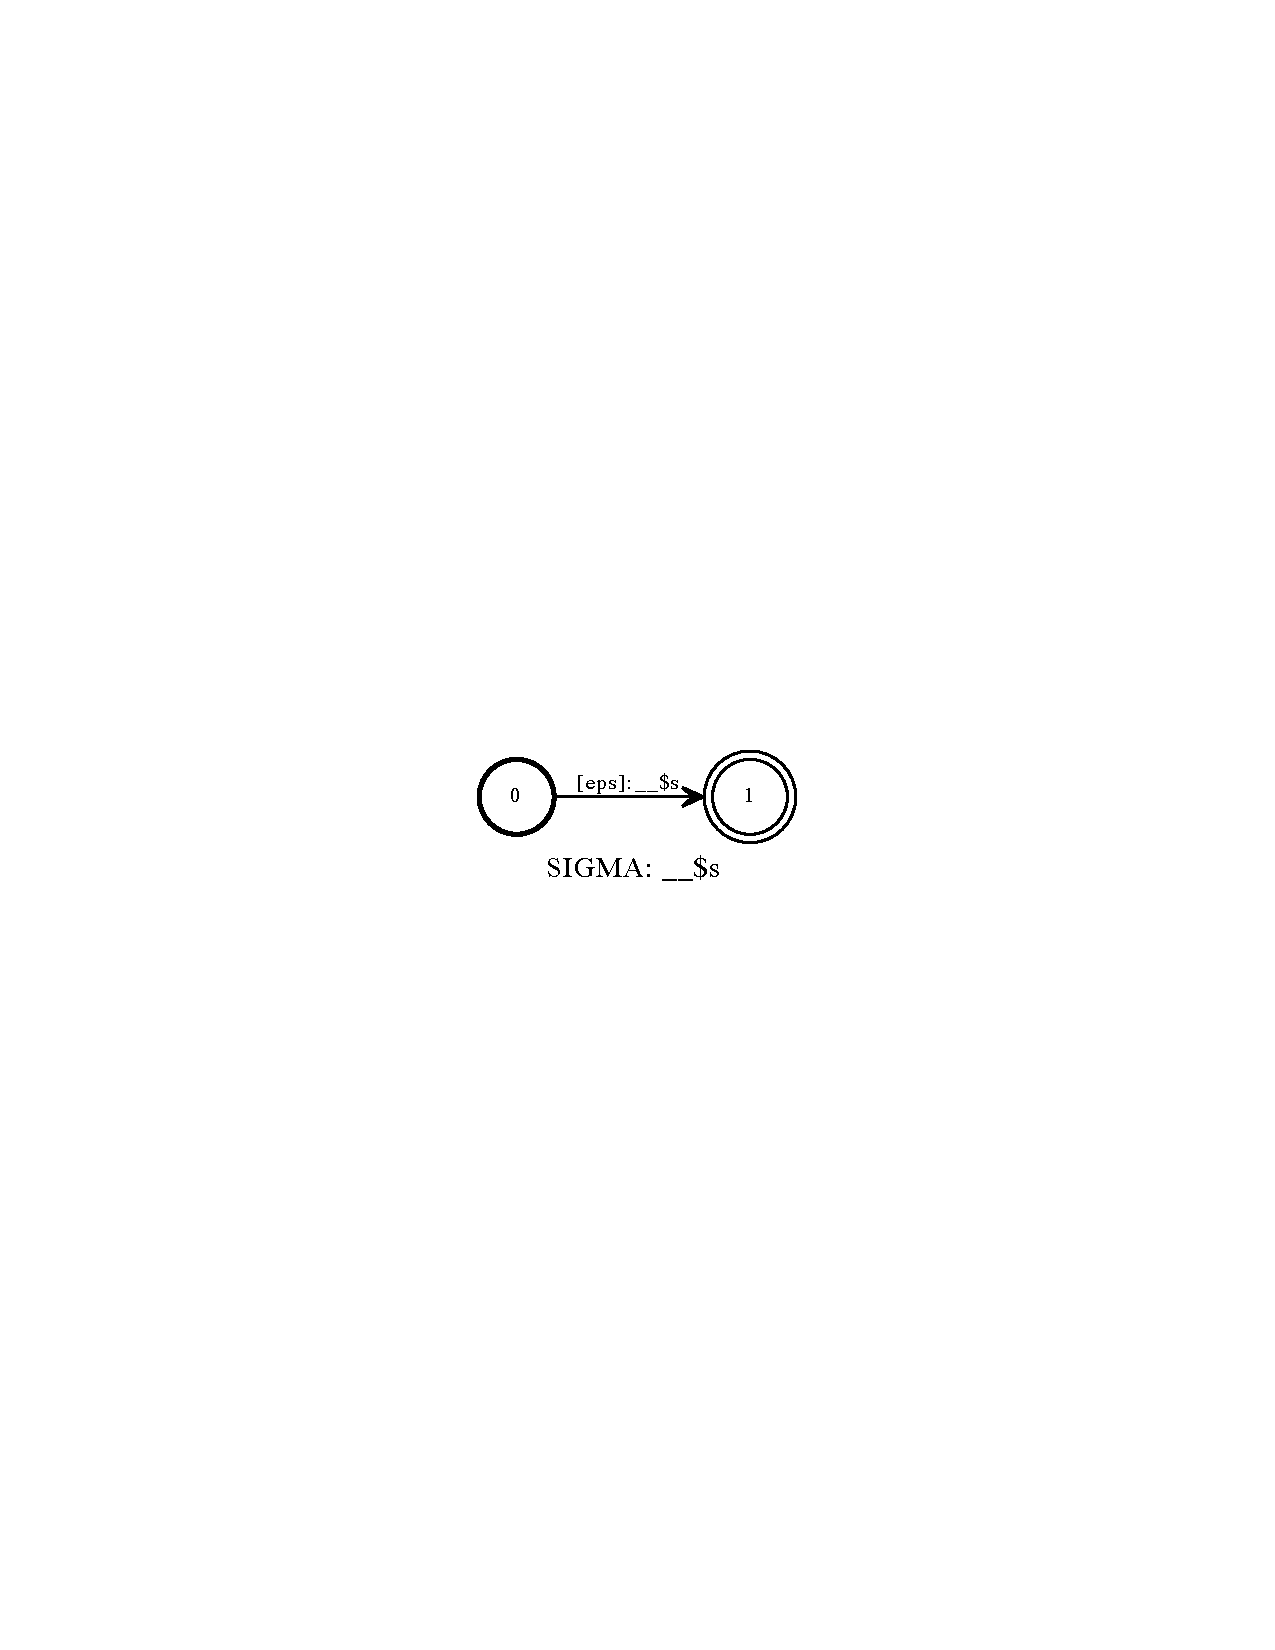
\includegraphics{images/reference.pdf}
\end{center}

\noindent
Currently in OpenFst, the symbol \verb!__$s! could in fact appear also on
the input side.  Of course, in the real network, the labels are really
just integers, 0 for epsilon, and some arbitrary value from the Private
Use Area for the multichar symbol.

Kleene programmers should use the wired-in \verb!$^sub()! function to
denote references to subnetworks and should not try to specify special
symbols like \verb!__$s! directly.  For example, the following statement
is illegal and will cause an exception to be thrown.

\begin{Verbatim}[fontsize=\small]
$rtn = "":'__$foo' ;    // raises an exception
\end{Verbatim}

\noindent
The use of \verb!$^sub()! at the programming level will also make it easy
for Kleene to adapt to any changes to \acro{rtn} representations that
might be made in the underlying OpenFst library.

\subsubsection{Embedding Subnetworks in an OpenFst \acro{rtn}}

The \verb!$^embedRtnSubnets($rtn)! function takes an OpenFst \acro{rtn}
argument, i.e.\@ a network that contains OpenFst-format references to
subnetworks, and returns a network that consists of the original network
unioned with a prefixed copy of each referred-to subnetwork.  For each
referred-to network \verb!$s!, the prefix consists of the special symbol
\verb!__SUBNETWORKS! followed by the special symbol \verb!__$s!.  Thus
from the following code

\begin{Verbatim}[fontsize=\small]
$p = p ;
$q = q ;
$rtn = a $^sub($p) b $^sub($q) ;
\end{Verbatim}

\noindent
the result \verb!$rtn! is this network containing two references to subnetworks

\begin{center}
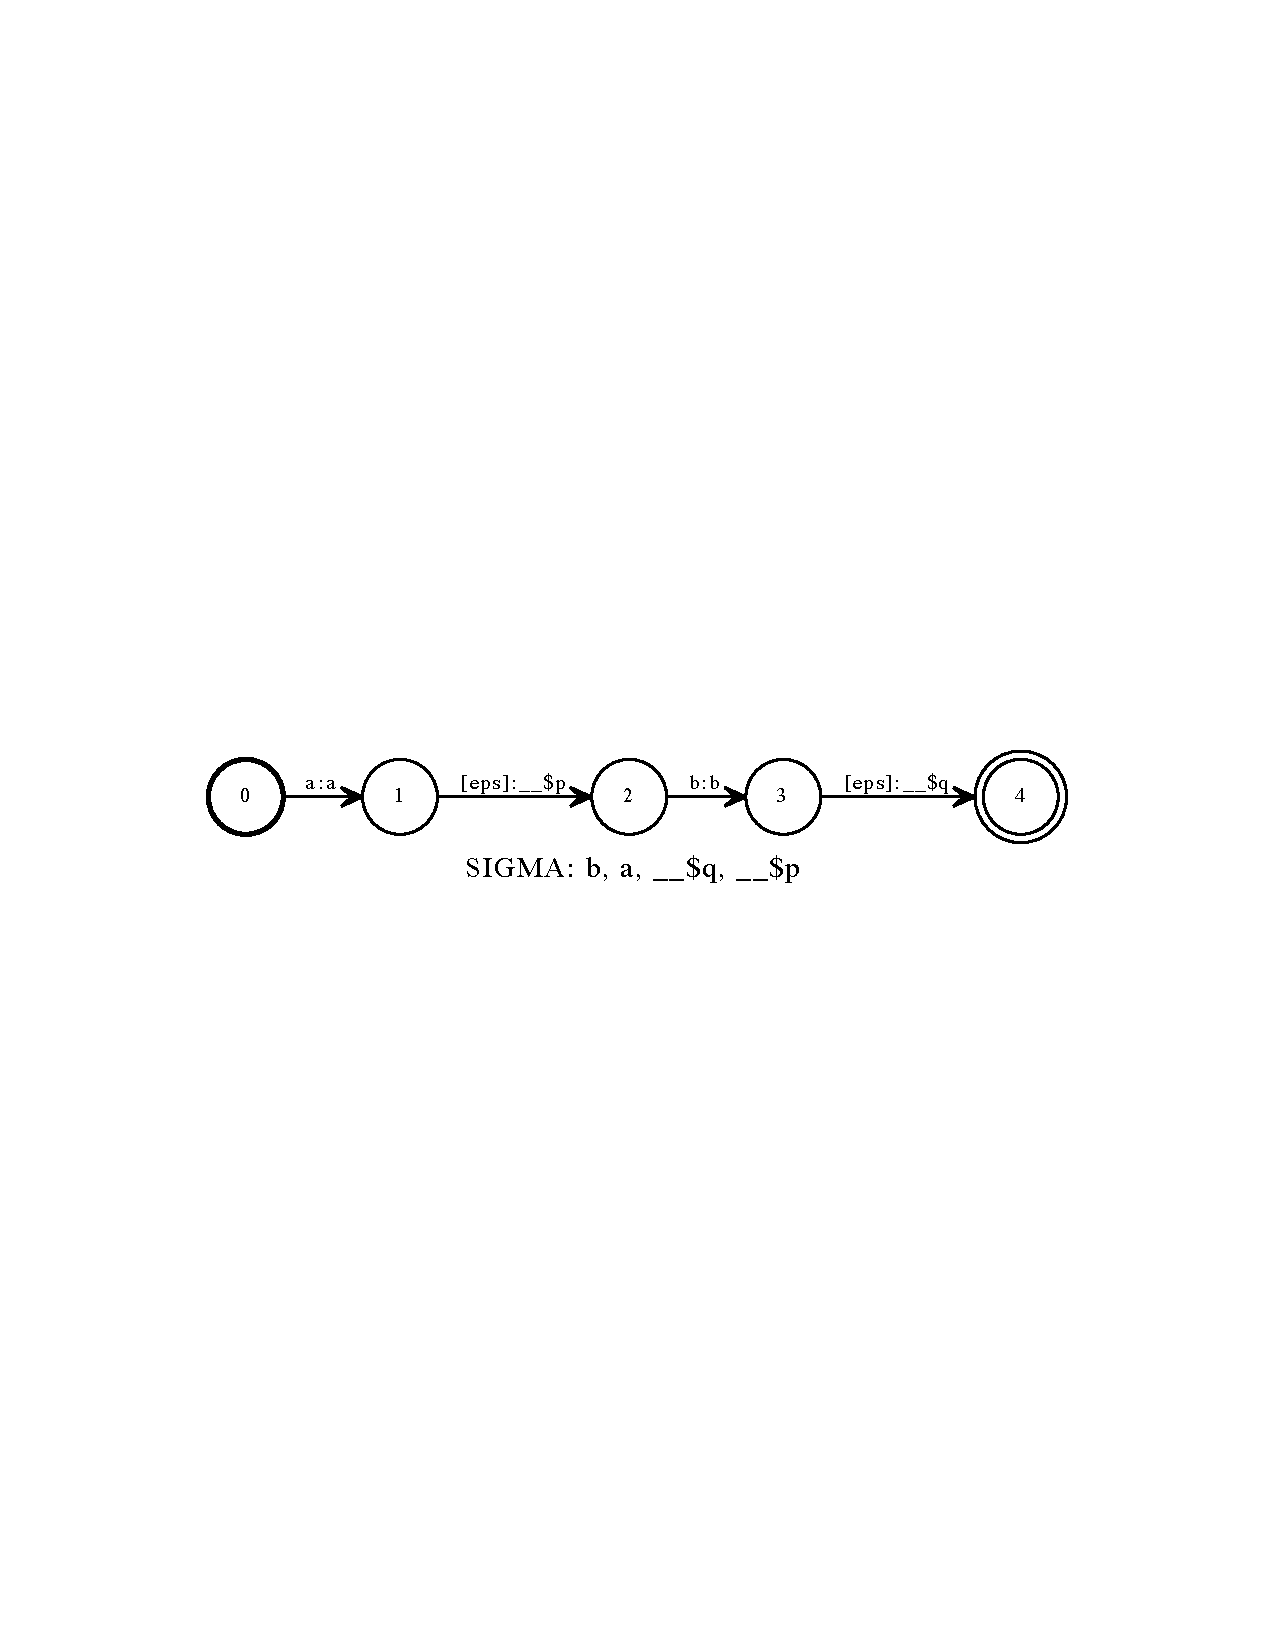
\includegraphics[width=\textwidth]{images/twoReferences.pdf}
\end{center}

\noindent
but the three referred-to networks remain separate.  After the following
call to \verb!$^embedRtnSubnets($rtn)!, 

\begin{Verbatim}[fontsize=\small]
$embedded = $^embedRtnSubnets($rtn) ;
\end{Verbatim}


\noindent
the resulting \verb!$embedded! network looks like this

\begin{center}
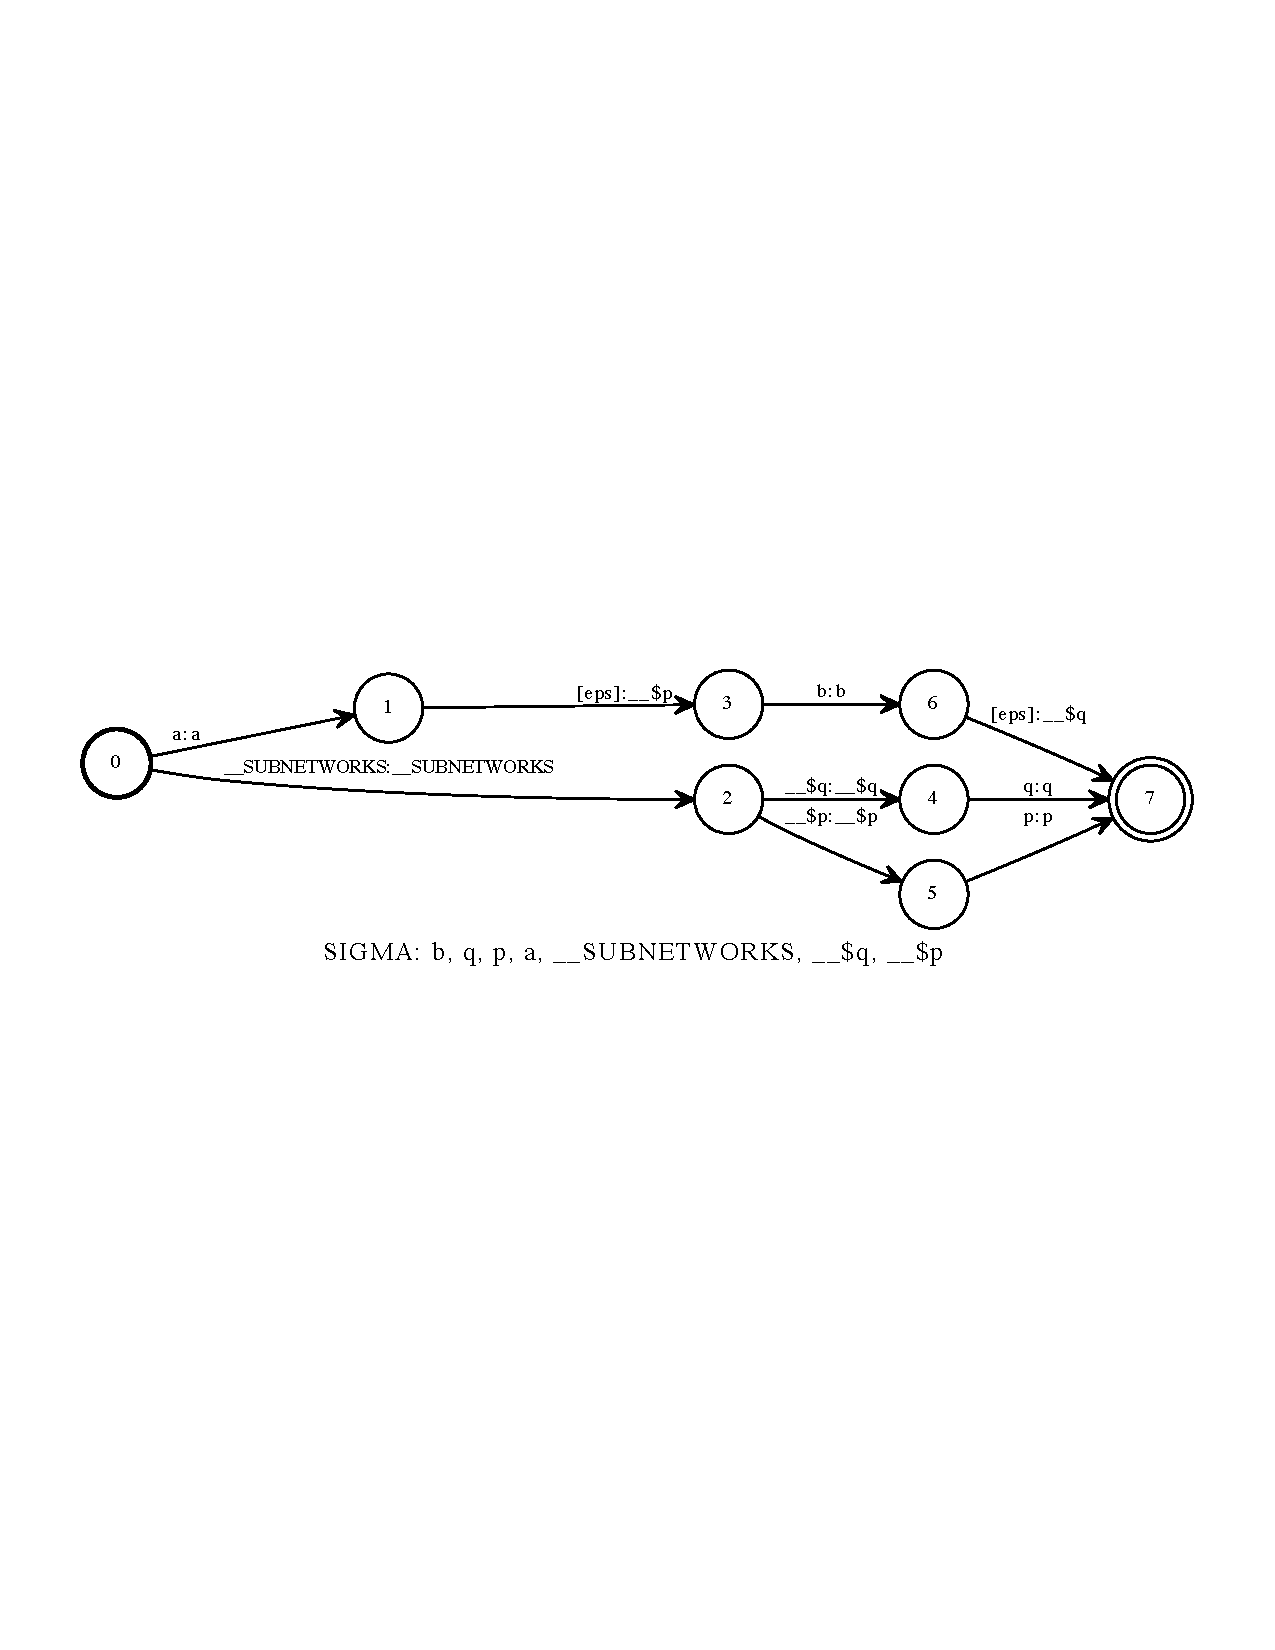
\includegraphics[width=\textwidth]{images/embedded.pdf}
\end{center}

\noindent
The embedded network can be saved to file as a single network and could be
applied by \acro{rtn}-savvy runtime code (not yet written) that knows the prefix convention.

The unioning of the base network with the subnetworks also guarantees that
the meaning of OTHER, if present, is standardized throughout all the
networks.

\subsubsection{Expanding an OpenFst \acro{rtn} into a Full Normal Network}

In some cases, it may also be useful to take an OpenFst \acro{rtn} and replace
each reference to a subnetwork with an actual copy of that subnetwork,
expanding the \acro{rtn} into a full normal network.  This is mathematically and
computationally possible only if the \acro{rtn} is regular.  Using the same
\verb!$rtn! example, a call to \verb!$^expandRtn()!

\begin{Verbatim}[fontsize=\small]
$expanded = $^expandRtn($rtn) ;
\end{Verbatim}

\noindent
produces the following \verb!$expanded! network

\begin{center}
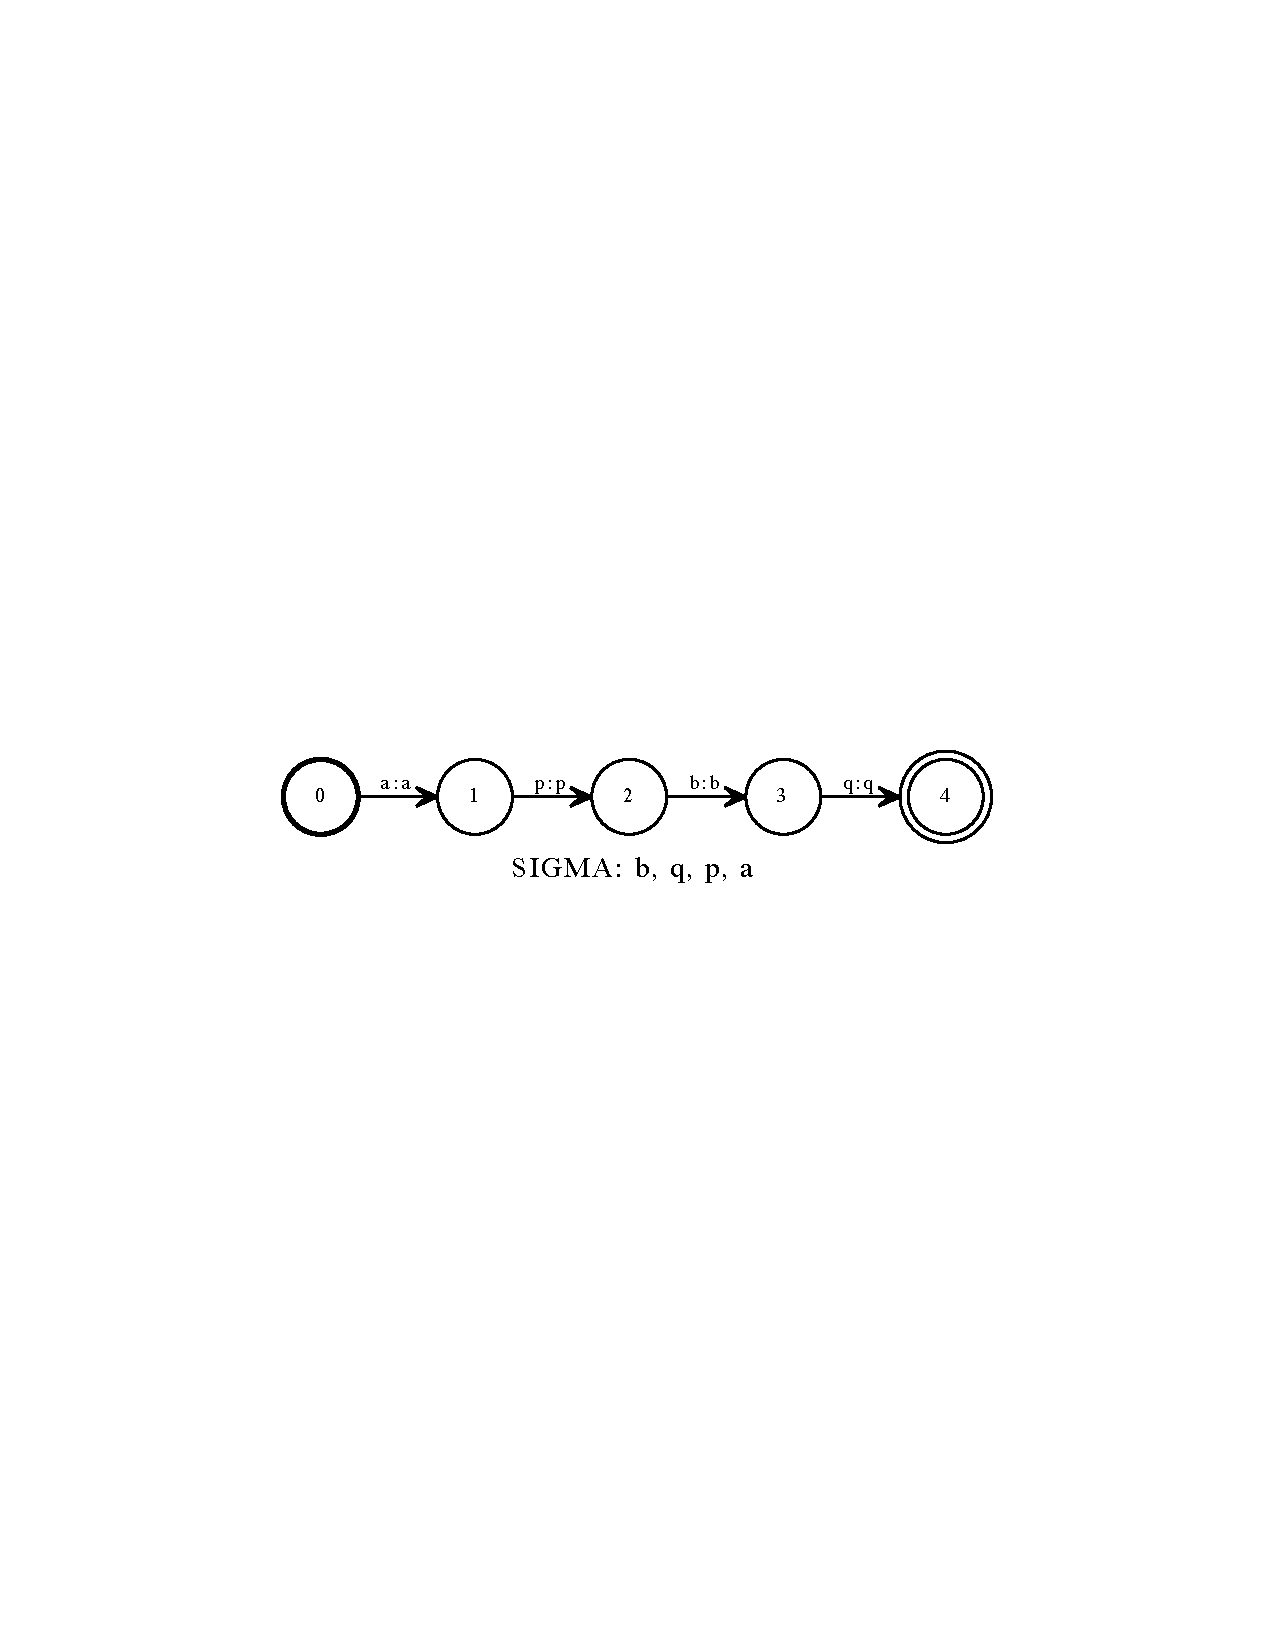
\includegraphics[width=\textwidth]{images/expanded.pdf}
\end{center}

\noindent
In real-life \acro{rtn}s, with multiple references to the same
subnetwork, the expanded network will be significantly bigger than the
original.  

If the \acro{rtn} contains cyclic references to subnetworks, it is
context-free in power (i.e.\@ no longer regular in power), and its
expansion would result in an infinite network.  The
\verb!$^expandRtn($rtn)! function checks for cyclic references and throws
an exception if the \verb!$rtn! is not regular.\footnote{In the OpenFst
library, the \verb!ReplaceFst()! operation provides a convenient method
that checks for cyclic references, and \verb!$^expandRtn()! invokes this
method.}

\section{\acro{sap} \acro{rtn} Support}

\label{sec:saprtn}

\subsection{Two Distinct Flavors of \acro{rtn} Support}

Kleene is currently being expanded to provide support for two distinct
flavors of Recursive Transition Networks or \acro{rtn}s.  This is work in
progress.

This section describes the current Kleene support for building
\acro{rtn}s using the \acro{sap} \acro{rtn} conventions, which are
compatible with the proprietary \acro{sap} \acro{rtn} runtime
code.\footnote{The \acro{sap} \acro{rtn} runtime code was written by Phil
Sours.  This runtime code is not currently available outside \acro{sap}.}
Non-\acro{sap} users wishing to create \acro{rtn}s compatible with the
OpenFst library should should ignore this section and proceed immediately
to section~\ref{sec:openfstrtn} starting on
page~\pageref{sec:openfstrtn}.

\subsection{\acro{sap} Recursive Transition Networks (\acro{rtn}s)}

\subsubsection{Status}

Kleene supports the building of Recursive Transition Networks
(\acro{rtn}s) that are compatible with proprietary \acro{sap} \acro{rtn}
runtime code.

An \acro{rtn} contains arc labels that are to be interpreted as
``references'' to subnetworks; and compatible \acro{rtn}-savvy runtime
code, when applying a network to data, will recognize such a reference
and ``push'' to the referenced subnetwork to continue the matching, and
then ``pop'' back to the calling network when the subnetwork has
successfully matched.  The references to subnetworks can also be thought
of as non-terminal labels.

\acro{rtn}s, containing references to subnetworks, are often smaller than
full-sized networks that must contain a full copy of each subnetwork
wherever it is needed.  However, \acro{rtn}s can denote context-free
languages, and so can go beyond regular power; a special subclass of
\acro{rtn}s remain regular.  The recognition/parsing of context-free
languages requires memory, in particular a push-down stack, and so any
runtime code to apply \acro{rtn}s must include such a stack.

\subsubsection{Predefined \acro{sap} Pattern Definitions}

\acro{sap} programmers writing patterns must start their source files, or
their interactive \acro{gui} sessions,  by sourcing the pre-defined
Kleene script \verb!PatternDefs.kl!.\footnote{This file may exist in
various versions, e.g.\@ \verb!PatternDefs-11.kl!.}

\begin{Verbatim}[fontsize=\small]
source "PatternDefs.kl" ;
\end{Verbatim}

\noindent
Alternatively, one can launch \Kleene{} and specify the script on the
command line:

\begin{Verbatim}[fontsize=\small]
$ java -jar Kleene.jar PatternDefs.kl -gui
\end{Verbatim}

\noindent
This script defines a set of useful Kleene functions for use by
\acro{sap} pattern writers, and it declares that any references to
subnetworks in an \acro{rtn} should be constructed according to the
\acro{sap} \acro{rtn} conventions.\footnote{The script
\verb!PatternDefs.kl! must contain the special Kleene command
\verb!SapRtnConventions!, which causes Kleene to build \acro{rtn}s
according to the proprietary \acro{sap} \acro{rtn} conventions.  The
typical \acro{sap} pattern writer will simply source
\verb!PatternDefs.kl! and will never need to specify or know about the
\verb!SapRtnConventions! command.} 

The sourcing of \texttt{PatternDefs.kl} at the beginning of a session
effectively turns \Kleene{} into what is known at \acro{sap} as the Pattern
Matching Language (\acro{pml}).

\subsubsection{Syntax for Creating an \acro{sap} \acro{rtn}}

For the \acro{sap} programmer, there needs to be a Kleene syntax to denote a
reference to a subnetwork, and it needs to be distinct from the syntax
that causes a copy of a network to be inserted.  For example, in this
example

\begin{Verbatim}[fontsize=\small]
$vowel = [aeiou] ;
$net = k $vowel t $vowel b $vowel ;
\end{Verbatim}

\noindent
the \verb!$vowel! network will be copied three times into \verb!$net!.  In
real-life applications, a subnetwork might encode something much larger, such
as the union of all nouns or even noun phrases in a natural language, and
multiple copies of such a subnetwork could easily
cause the final network to become very large, or even too large to
compute.

Kleene currently supports a wired-in function \verb!$^sub($s)! that
programmers can use to denote a reference to a subnetwork.\footnote{I'm
not tied to the spelling \verb!$^sub($s)! and would be comfortable with
alternatives such as \verb!$^ref($s)! or \verb!$^push($s)!, or even some
special syntax like \verb!>$s<! or \verb!>>$s!.}  To continue with our
trivial example, 

\begin{Verbatim}[fontsize=\small]
source "PatternDefs.kl" ;

$vowel = [aeiou] ;
$rtn = k $^sub($vowel) t $^sub($vowel) b $^sub($vowel) ;
\end{Verbatim}

\noindent
this would result in an \verb!$rtn! network that contains three compact
one-label references to the subnetwork \verb!$vowel! rather than three
full copies of it.  In real-life applications, the savings in memory can
be very significant.

As shown in this example, the \acro{sap} pattern writer should source the
script \verb!PatternDefs.kl!, one way or another, before creating any
networks intended for use with the \acro{sap} \acro{rtn} runtime
code.\footnote{If \verb!PatternDefs.kl! is not sourced, the calls to
\verb!$^sub()! will create references to subnetworks that are not
compatible with the \acro{sap} runtime code but, rather, are compatible
with the native support for \acro{rtn}s provided by OpenFst (see
\ref{sec:openfstrtn}).}

\subsubsection{What does a Reference Look Like in an \acro{sap} \acro{rtn}?}

Networks consist of states and arcs, and each arc has two labels, an
input label, and an output label.\footnote{The terminology of
\emph{input} and \emph{output} labels is that of the OpenFst tradition.
In the Xerox tradition, they are called \emph{upper} and \emph{lower},
respectively, or sometimes \emph{lexical} and \emph{surface}.}  In the
actual network, the labels are really integers, and all Unicode
characters, such as \emph{a}, \emph{b}, \emph{c}, etc.\@ are represented
using their standard Unicode code point value.  Multichar symbols are
stored using a code point value selected at random from a Unicode Private
Use Area.

To be compatible with the \acro{sap} \acro{rtn} runtime code, a reference
to a subnetwork \verb!$s! is the multichar symbol \verb!'$s'!, which,
internally, is just an integer.  The identity network label
\verb!'$s':'$s'! tells the \acro{sap} runtime code to perform a simple
``push'' to subnetwork \verb!$s!, to match \verb!$s! against the input,
and to produce the output of \verb!$s!, which may be an acceptor or a
transducer.  The Kleene syntax \verb!$^sub($s)!, \verb!'$sub'!, or
\verb!'$sub':'$sub'! results in an arc label \verb!'$s':'$s'!.

The \acro{sap} \acro{rtn} runtime code can also match a subnetwork
against the input symbols and output epsilon---i.e.\@ the empty string.
When the runtime code is told to apply the \acro{rtn} in a ``downward''
direction, matching input symbols against the input/upper side, the
network label \verb!'$s':$eps! tells the runtime code to push to
subnetwork \verb!$s! and to map the output to epsilon, effectively
suppressing the output.  Similarly, when the runtime code is told to
apply the \acro{rtn} in a ``upward'' direction, matching input symbols
against the output/lower side, the network label \verb!$eps:'$s'! tells
the runtime code to push to subnetwork \verb!$s! and to map the output to
epsilon, again suppressing the output.  This mapping-to-epsilon is
performed inside the \acro{sap} \acro{rtn} runtime code.

Using real code examples, under \acro{sap} \acro{rtn} conventions, the syntax

\begin{Verbatim}[fontsize=\small]
$rtn = $^sub($s) ;
\end{Verbatim}

\noindent
results in a simple \verb!'$s':'$s'! label.  \acro{sap} programmers can
also program this more directly as

\begin{Verbatim}[fontsize=\small]
$rtn = '$s' ;
\end{Verbatim}

\noindent
using the normal Kleene syntax for multichar symbols.


To specify an input/upper-side reference to \verb!$s!, with mapping to
epsilon, the syntax is \verb!$^sub($s):""!, \verb!$^sub($s):$eps!,
\verb!'$sub':""!, \verb!'$sub':$eps!, etc.

\begin{Verbatim}[fontsize=\small]
$rtn = $^sub($s):$eps ;
\end{Verbatim}

\acro{sap} references to subnetwork can be either simple identity
mappings, e.g.\@ \verb!'$s':'$s'!, or mappings to epsilon,
\verb!'$s':$eps! or \verb!$eps:'$s'!.  Any attempt to map a subnetwork
reference \verb!$s! to anything other than itself or epsilon will raise
an exception.

\begin{Verbatim}[fontsize=\small]
$badrtn1 = '$sub':x ;  // illegal
$badrtn2 = x:'$sub' ;  // illegal
\end{Verbatim}

\subsubsection{Embedding Subnetworks in an \acro{sap} \acro{rtn}}

The \verb!$^embedRtnSubnets($rtn)! function takes an \acro{sap}
\acro{rtn} argument, i.e.\@ a network that contains \acro{sap}-format
references to subnetworks, and returns a network that consists of the
original network unioned with a prefixed copy of each referred-to
subnetwork.  For each referred-to network \verb!$s!, the prefix consists
of the special symbol \verb!__SUBNETWORKS! followed by the special symbol
\verb!$s!.  Thus from the following code

\begin{Verbatim}[fontsize=\small]
$p = p ;
$q = q ;
$rtn = a $^sub($p) b $^sub($q) ;
\end{Verbatim}

\noindent
the result \verb!$rtn! is this network containing two references to subnetworks

\begin{center}
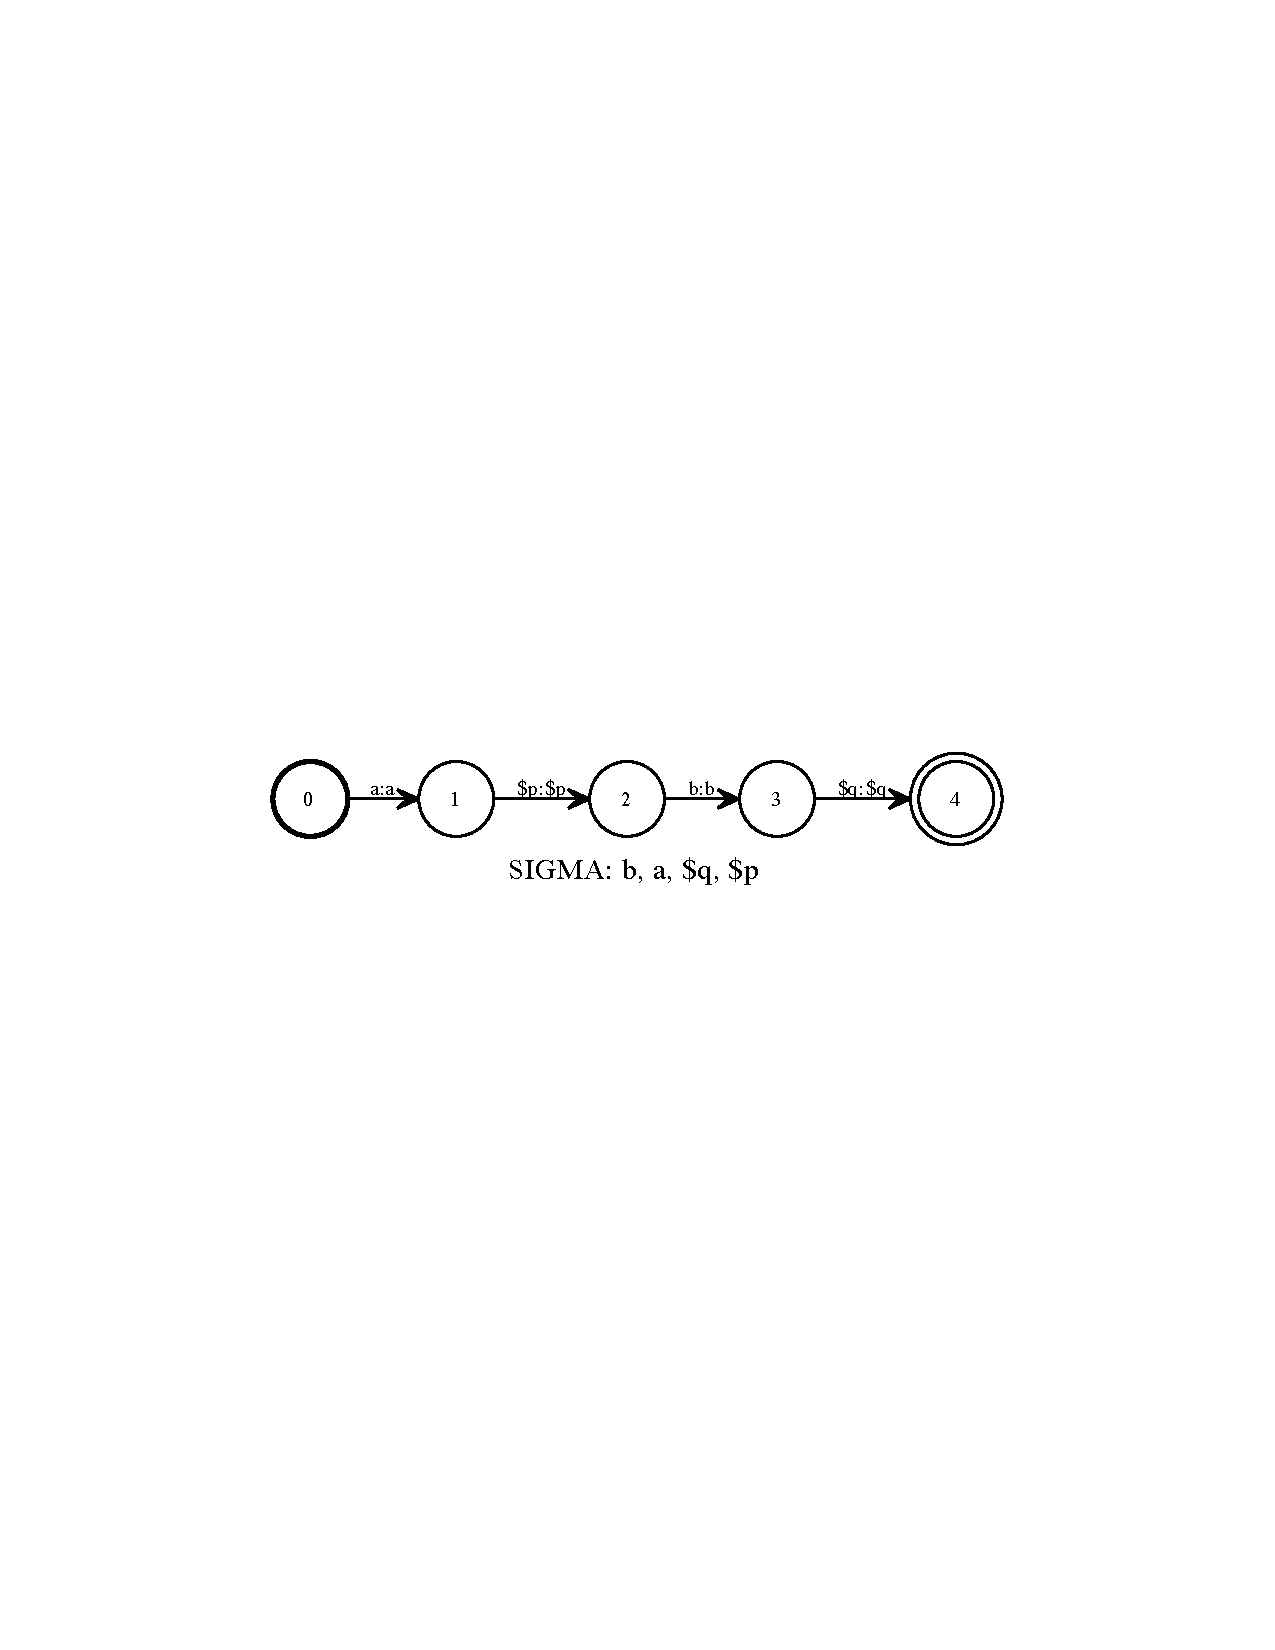
\includegraphics[width=\textwidth]{images/sapTwoReferences.pdf}
\end{center}

\noindent
but the three referred-to networks remain separate.  After the following
call to \verb!$^embedRtnSubnets($rtn)!, 

\begin{Verbatim}[fontsize=\small]
$embedded = $^embedRtnSubnets($rtn) ;
\end{Verbatim}


\noindent
the resulting \verb!$embedded! network contains a single copy of each
referred-to subnetwork looks like this

\begin{center}
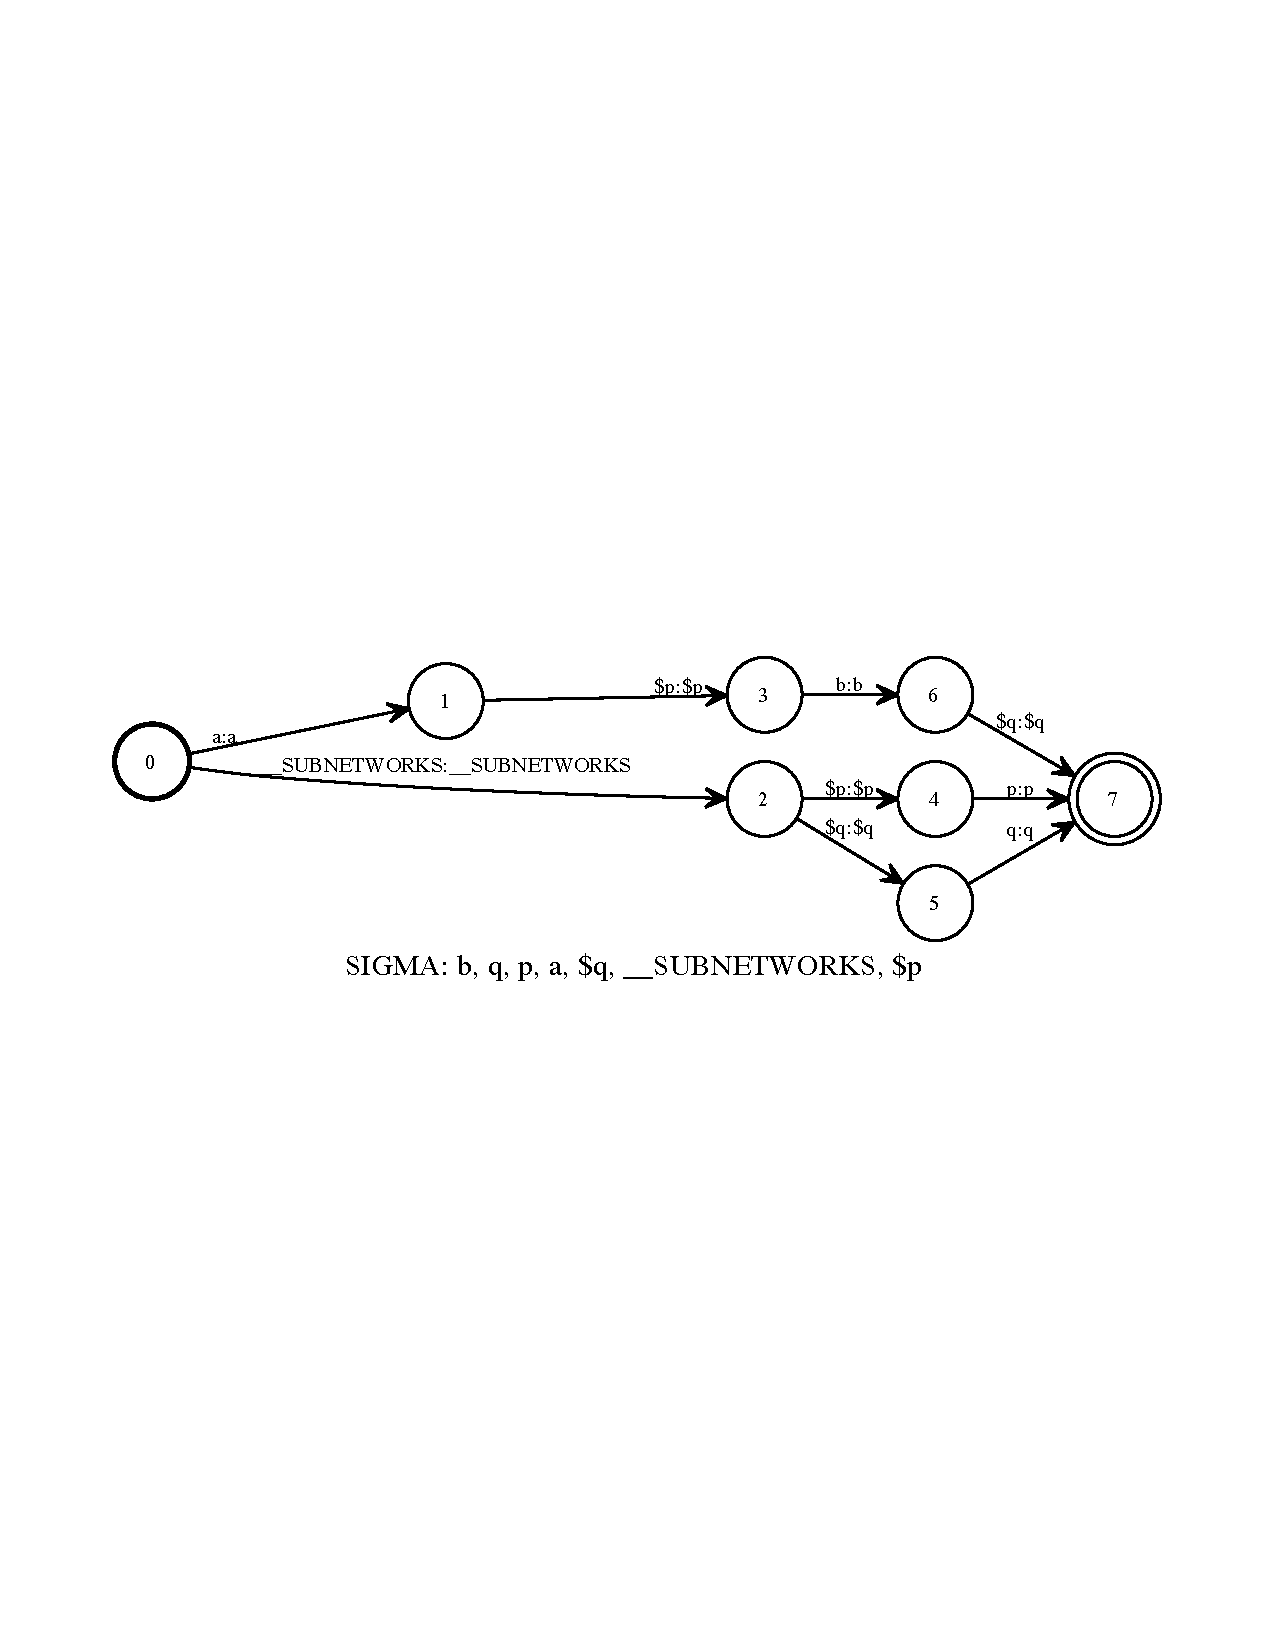
\includegraphics[width=\textwidth]{images/sapEmbedded.pdf}
\end{center}

\noindent
An embedded network can be saved to file as a single network and is
applied by \acro{sap}-\acro{rtn}-savvy runtime code that knows the label-prefix
conventions.  
The unioning of the base network with the subnetworks also guarantees that
the meaning of OTHER, if present, is standardized throughout all the
networks.

When the references are mapped to epsilon, 

\begin{Verbatim}[fontsize=\small]
$p = p ;
$q = q ;
$rtn = a $^sub($p):$eps b $^sub($q):$eps ;
\end{Verbatim}

\noindent
the reference labels look slightly different.

\begin{center}
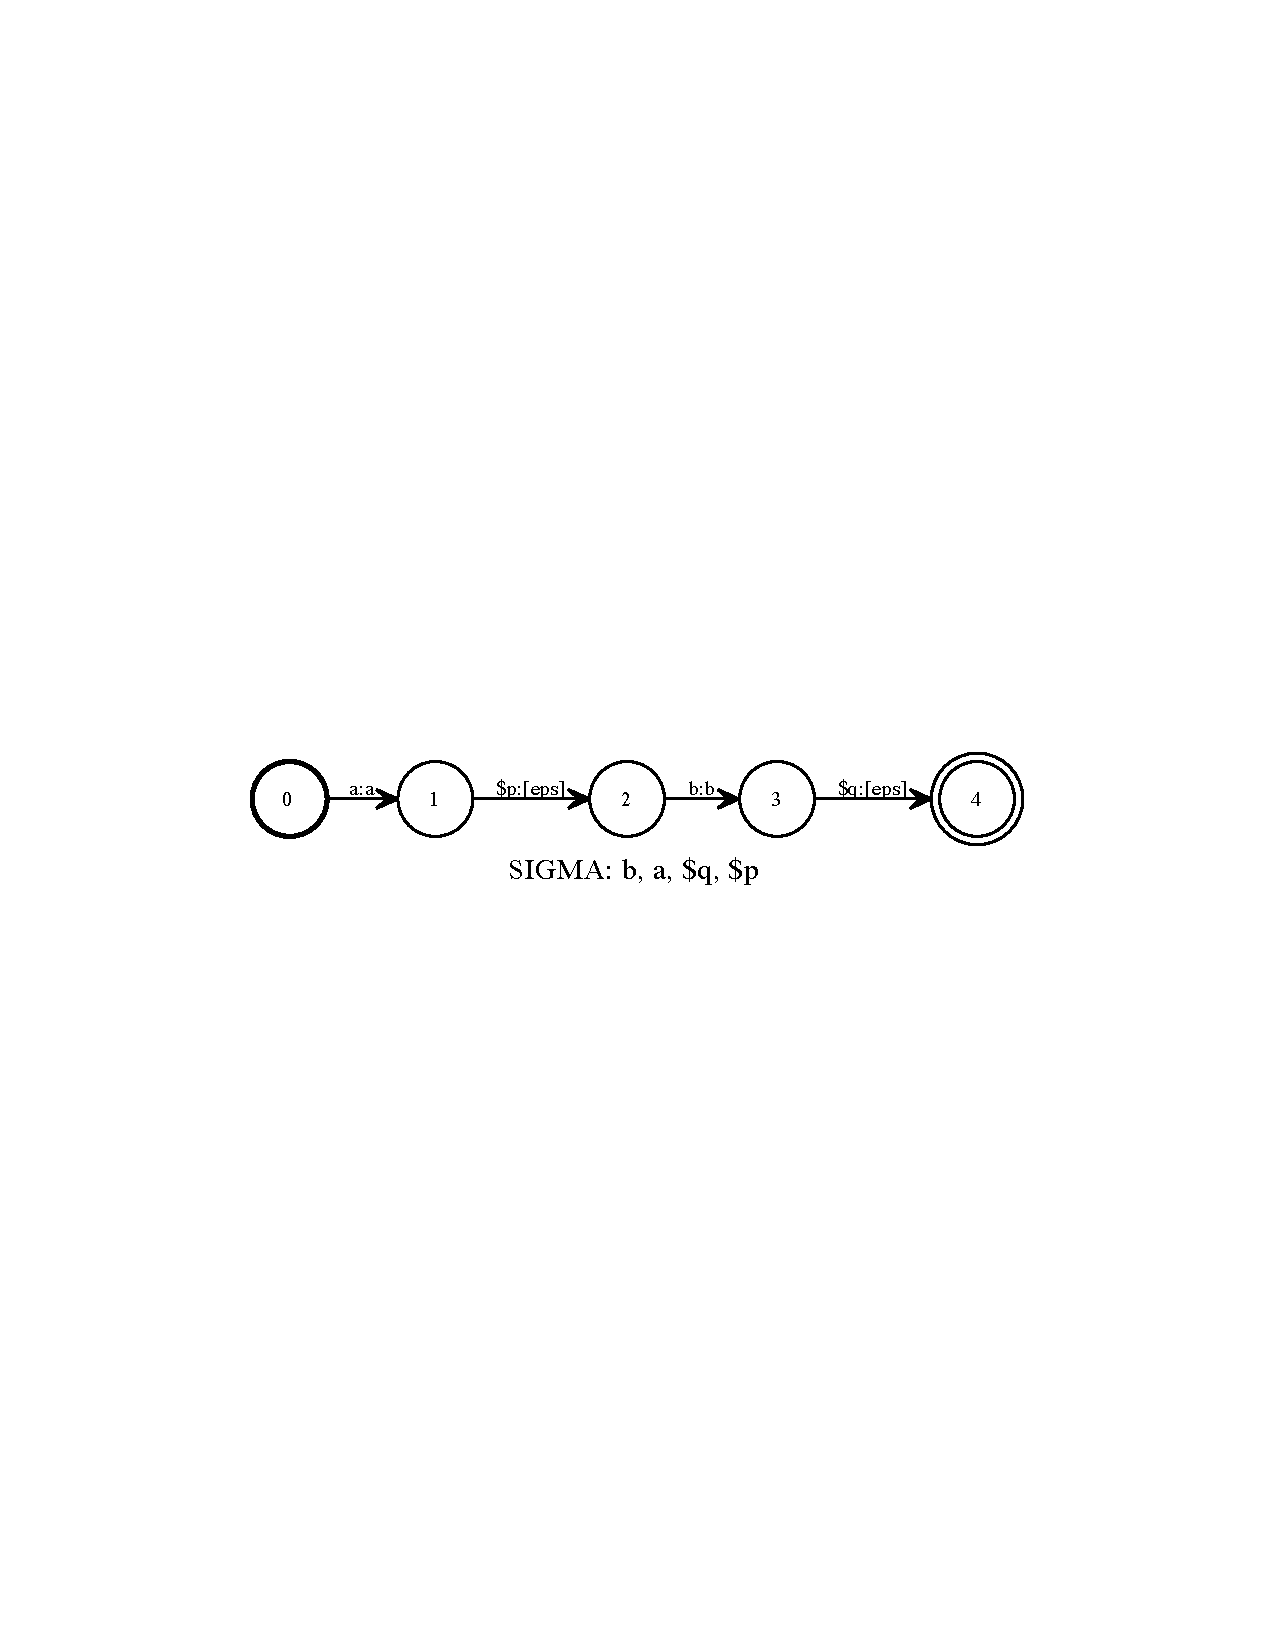
\includegraphics[width=\textwidth]{images/sapEpsTwoReferences.pdf}
\end{center}

However, when the referred-to networks are embedded, the embedded networks and their
prefixes are the same as before.

\begin{Verbatim}[fontsize=\small]
$embedded = $^embedRtnSubnets($rtn) ;
\end{Verbatim}


\begin{center}
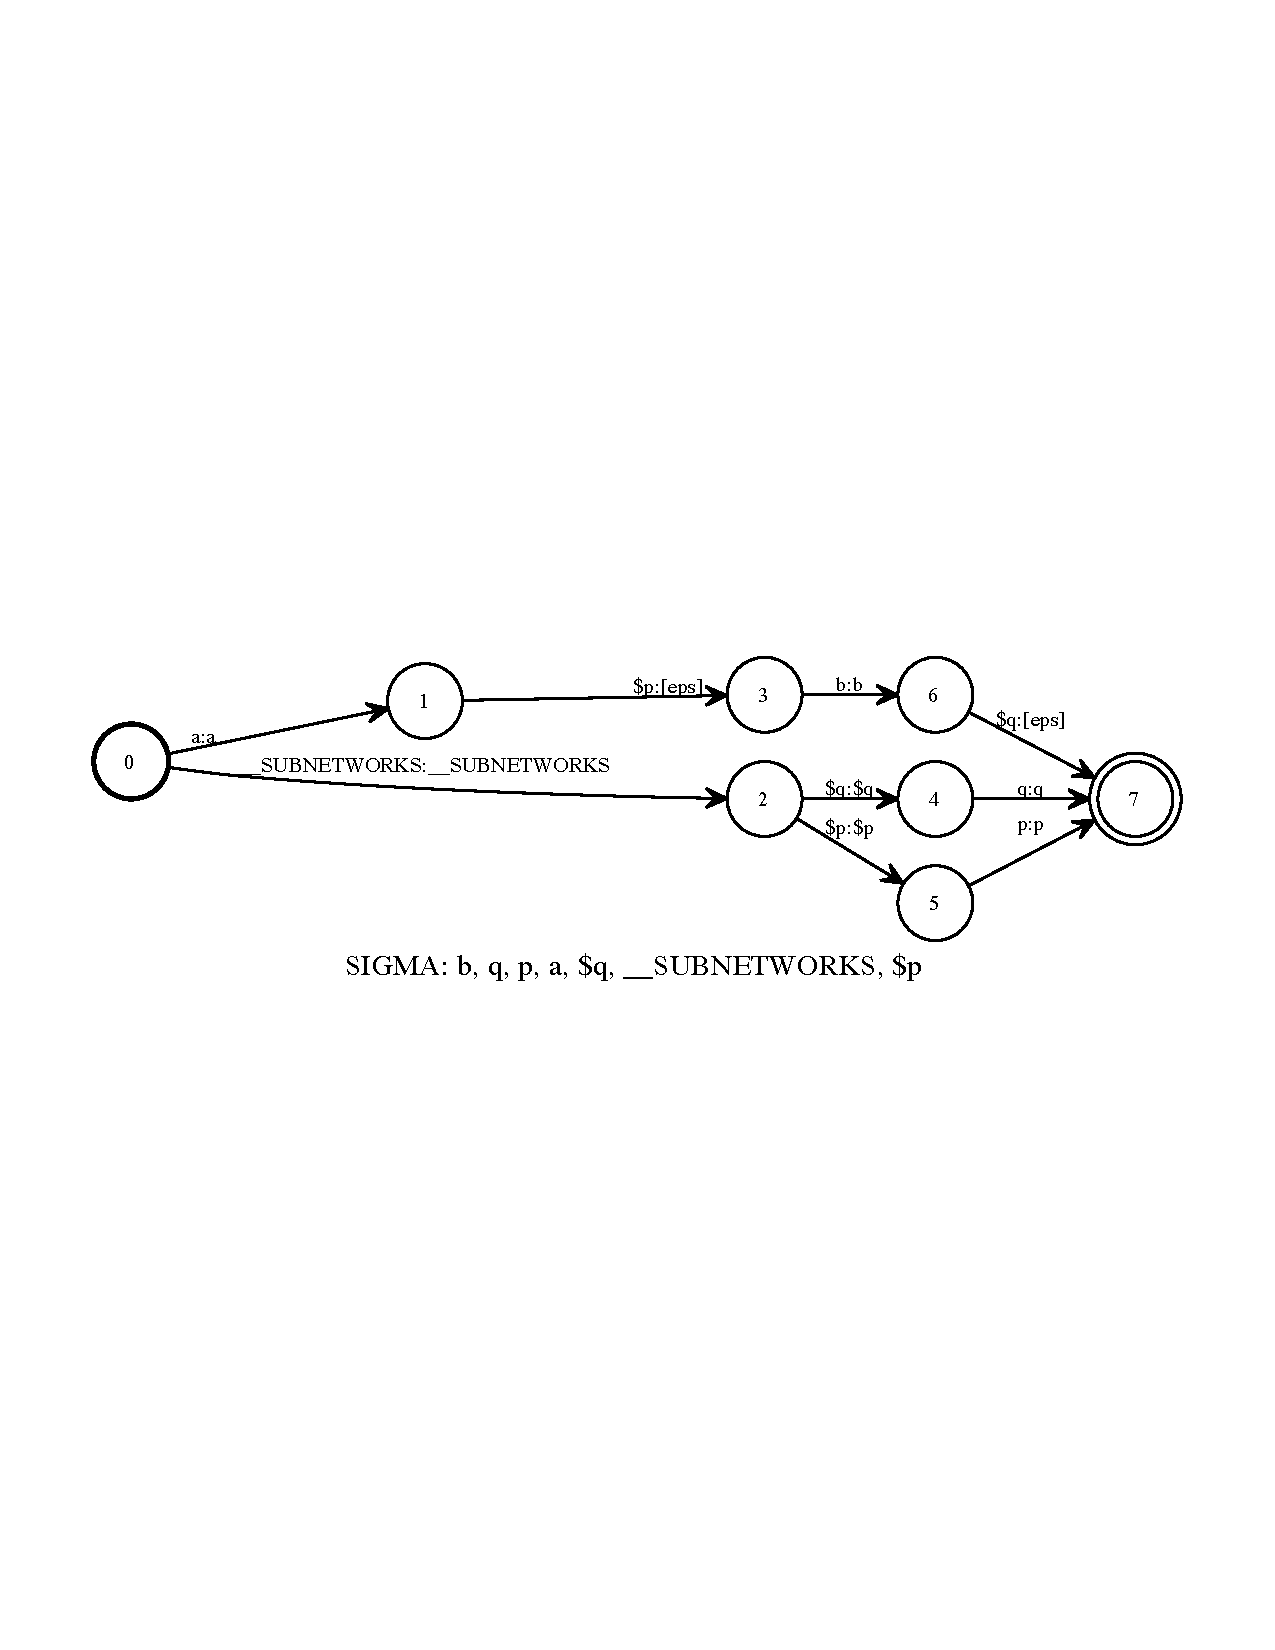
\includegraphics[width=\textwidth]{images/sapEpsEmbedded.pdf}
\end{center}

An embedded network is effectively a ``final'' network, and
programmers should avoid subjecting it to some operations like
\verb!$^reverse()!, which will create an unusable result.

\subsubsection{Expanding an \acro{sap} \acro{rtn} into a Full Normal Network}

At this time, the expansion of an \acro{sap}-format \acro{rtn} into a full normal network
is not supported.\footnote{\acro{sap}-format \acro{rtn}s can contain special references
to subnetworks, wherein the runtime code maps the output to epsilon.  This special
mapping, performed inside the runtime code, is not currently compatible with the
off-the-shelf \verb!Replace()! and \verb!ReplaceFst()! operations provided by OpenFst.
In the future, we may write new versions of these library functions that support
expansion of \acro{sap} \acro{rtn}s.}

\subsubsection{Semantic Constraints in Kleene on Operations for \acro{sap} \acro{rtn}s}

\label{sec:saprtnrestrictions}

\paragraph{Semantic Constraints.}

There are numerous semantic constraints on the operations that can be performed on
\acro{sap} \acro{rtns}.  Kleene identifies \acro{rtn}s during interpretation and throws
exceptions when illegal operations are attempted on them.

\paragraph{Crossproduct.}

In \acro{sap} \acro{rtn}s, a reference to a subnetwork can a simple reference,
as with \verb!'$foo'! in 

\begin{Verbatim}[fontsize=\small]
$rtn = a b '$foo' c ;
\end{Verbatim}

\noindent
which tells the \acro{sap} \acro{rtn} runtime code to match subnetwork 
\verb!$foo! against the input and produce whatever \verb!$foo! outputs.
Alternatively, a reference written as the crossproduct, e.g.\@
\verb!'$foo':$eps! or,
equivalently,
\verb!'$foo':""! tells the runtime code to match subnetwork 
\verb!$foo! against the input but to map
the output to epsilon, the empty string.

\begin{Verbatim}[fontsize=\small]
$rtn = a b '$foo':"" c ;
\end{Verbatim}

The use of crossproduct with \acro{sap} \acro{rtn}s is limited to having
references to subnetworks on one side, and epsilon on the other side.
Thus the examples

\begin{Verbatim}[fontsize=\small]
$rtn1 = '$foo':"" ;
$rtn2 = (a '$foo' b):"" ;
$rtn3 = "":'$foo' ;
$rtn4 = "":(a '$foo' b) ;
\end{Verbatim}

\noindent
are legal crossproducts, but

\begin{Verbatim}[fontsize=\small]
$bad1 = '$foo':z ;  // illegal mapping to z rather than epsilon
$bad2 = a:'$foo' ;  // illegal mapping to a rather than epsilon
\end{Verbatim}

\noindent
are illegal crossproducts, and Kleene will throw an exception.

\paragraph{Legal and Illegal Operations on \acro{rtn}s.}

The following chart summarizes the operations that definitely can and
cannot be performed on \acro{sap} \acro{rtn}s.

\vspace{.5cm}

\noindent
\begin{tabular}{|l|c|p{5.7cm}|}
\hline
\textbf{Operation} & \textbf{Operator(s)} & \textbf{Comment} \\
\hline
\hline
crossproduct & : & Limited to identity labels, or mapping to epsilon (see
above)\\
\hline
iteration & \verb!* + ?! {} & Legal \\
\hline
concatenation & & Legal \\
\hline
union & | & Legal \\
\hline
\hline
composition & \verb!_o_! & Illegal \\
\hline
complementation & \verb!~! & Illegal \\
\hline
subtraction & - & Illegal \\
\hline
intersection & \verb!&! & Illegal \\
\hline
shortestPath & \verb!$^shortestPath(!\ldots\verb!)! & Illegal \\
\hline
\end{tabular}

\vspace{.5cm}

\noindent
When Kleene detects that an illegal operation is being attempted on one or more
\acro{rtn} arguments, it throws a runtime exception.


The \verb!$^shortestPath($fst, #nshortest=1)! function returns the
network containing the nshortest ``best'' paths from the input
\verb!$fst!.\footnote{The terminology and behavior of
\verb!$^shortestPath($fst, #nshortest=1)! is taken from the
\verb!ShortestPath()! function of the underlying OpenFst library.}  

Under the Tropical Semiring, wherein weights are costs, the best paths
have the lowest costs.  By default, the second argument has the value of
1.  If the input network contains m lowest-cost paths of the same weight,
and \texttt{nshortest} is less than m, only \texttt{nshortest} paths,
chosen at random, will be returned.  

\paragraph{Cautions on Operations.}

Certain operations on \acro{sap} \acro{rtn}s are legal but semantically 
questionable, and
they should be used with caution.

\vspace{.5cm}

\noindent
\begin{tabular}{|l|p{9cm}|}
\hline
\textbf{Operation} & \textbf{Caution} \\
\hline
\hline
\verb!$^determinize()! & useful but not strictly correct at the symbol level \\
\hline
\verb!$^minimize()! & useful but not strictly correct at the symbol level \\
\hline
\verb!$^rmEpsilon()! & useful but not strictly correct at the symbol level \\
\hline
\hline
\verb!$^rmWeight()! & legal, but the user should also process subnetworks \\
\hline
\verb!$^reverse()! & legal, but the user should also process subnetworks \\
\hline
\verb!$^substSymbol()! & legal, but the user should also process subnetworks \\
\hline
\verb!$^invert()! & legal, but the user should also process subnetworks \\
\hline
\verb!$^inputside()! & legal, but the user should also process subnetworks \\
\hline
\verb!$^outputside()! & legal, but the user should also process subnetworks \\
\hline
\end{tabular}

\vspace{.5cm}

\noindent
Kleene does not throw exceptions for these questionable operations, and it is
up to the user to process the main \acro{rtn} and any referred-to subnetworks
in appropriate ways.  For example, for an \acro{rtn} defined as

\begin{Verbatim}[fontsize=\small]
$rtn = a <0.1> b <0.2> '$sub' c <0.3> ;
$urtn = $^rmWeight($rtn) ;
\end{Verbatim}

\noindent
the call to \verb!$^rmWeight()! is legal and potentially useful, but the
referred-to subnetwork \verb!$sub! may be referred
to by multiple \acro{rtn}s, or may not even be defined yet, so it cannot be
un-weighted automatically along with the main \verb!$rtn!.  For more
information on how \acro{rtn}s are marked, and how semantic problems are
detected during interpretation, see Appendix~\ref{app:rtn}.

\section{Unicode Support}

\subsection{Kleene, Java and Unicode}

The Kleene parser is a Java program, and Kleene supports Unicode to the extent (and
in the same way) that any Java program supports Unicode, which is pretty well---but
not perfectly.\footnote{The Unicode Standard (\url{http://www.unicode.org})
is mature and very comprehensive, but
the \emph{implementation} of Unicode in programming languages, 
text editors, \acro{gui} libraries,
typesetting packages, and other text-handling software varies considerably in completeness
and reliability.}  The
Kleene \acro{gui} is written using the Java Swing library, and Swing text
widgets---including JTextField and JTextArea---are automatically Unicode-friendly.  

\subsection{Kleene Scripts and Unicode}

\subsubsection{The Default Encoding of the Operating System}

Pre-edited Kleene scripts can be run from the command line, or from the \acro{gui}.
It is \emph{not} required that Kleene scripts be stored as Unicode---Kleene can
read and execute scripts written in a huge number of standard encodings, converting the text to Unicode for
internal processing.  If Kleene is told to run a script, and if the encoding of that script is not
explicitly specified, then by default it will assume that the script is in the
default encoding of the operating system, whatever that might be.

\begin{Verbatim}[fontsize=\small]
$ java -jar Kleene.jar myscript
\end{Verbatim}

\noindent
In this example, \texttt{myscript} would be assumed to be stored in the default encoding
of the operating system and would be opened and read as such, with Java performing
an automatic conversion of the text from that default encoding to Java's internal
Unicode encoding, which happens to be \acro{utf}-16.

Note that Kleene does not attempt to analyze the input file and detect what its encoding
might be from internal evidence.  Rather it interrogates the operating system to
find the default encoding, and it attempts to open and read the file accordingly.  If, for some reason,
the input file is not in the default encoding of the operating system, the input
may result in a warning message or garbling.

In a Unix-like system, the default encoding of the operating system can be seen by
entering \texttt{locale} at the command line:

\begin{Verbatim}[fontsize=\small]
$ locale
\end{Verbatim}

\noindent
On any system, the default encoding, as seen by a Java program, can also be revealed by compiling
and running the following trivial Java script, which should be in a file named
\texttt{FindDefaultEncoding.java}.

\begin{Verbatim}[fontsize=\small]
public class FindDefaultEncoding {
    public static void main(String[] args) {
        String s = System.getProperty("file.encoding") ;
        System.out.println(s) ;
    }
}
\end{Verbatim}

\noindent
To compile and run this script, do the following:

\begin{Verbatim}[fontsize=\small]
$ javac FindDefaultEncoding.java
$ java FindDefaultEncoding
\end{Verbatim}

On \acro{os x} even if the locale has been set to some specified
encoding, such as \acro{utf-8}, the call to
\verb!System.getProperty("file.encoding")! will still, unfortunately,
return MacRoman.\footnote{Curiously, in the Groovy and Scala
languages, which are, like Java, based on the Java Virtual Machine
(\acro{jvm}), this problem appears to have been fixed.  On a
system where the locale is set to \acro{utf-8}, executing
\texttt{println (System.getProperty("file.encoding"))} in Scala
2.8.1 or Groovy 1.7.5 returns \verb!"UTF-8"!.}  This can be overcome by calling any Java program with a
\verb!-D! option specifying the desired default
encoding.

\begin{Verbatim}[fontsize=\small]
$ javac FindDefaultEncoding.java
$ java -Dfile.encoding=UTF-8 FindDefaultEncoding
\end{Verbatim}

\subsubsection{Running Scripts in Any Standard Encoding}

Regardless of the default encoding of the operating system, Kleene can
run scripts in any standard encoding as long as that encoding is
explicitly specified using the \texttt{-encoding} flag.\footnote{This
\texttt{-encoding} flag, and its semantics, are copied from the same flag
used for the \texttt{javac} compiler; see
\url{http://java.sun.com/j2se/1.5.0/docs/tooldocs/windows/javac.html}.}
So if the script is, for some reason, stored in an encoding that is not
the default encoding of the operating system, it is necessary to specify
that encoding as in the following examples: 

\begin{Verbatim}[fontsize=\small]
$ java -jar Kleene.jar -encoding UTF-8      myscript
$ java -jar Kleene.jar -encoding UTF-16     myscript
$ java -jar Kleene.jar -encoding Latin-1    myscript
$ java -jar Kleene.jar -encoding ISO-8859-1 myscript
$ java -jar Kleene.jar -encoding ISO-8859-6 myscript
$ java -jar Kleene.jar -encoding EUC-JP     myscript
\end{Verbatim}

\subsubsection{A Plug for Unicode}

All things being equal, users working on languages with orthographies
that cannot be represented in \acro{ascii} are highly encouraged to use
Unicode rather than resorting to obsolete 8-bit encodings or, especially,
to Roman transliterations that may have been required in pre-Unicode
software.\footnote{The \acro{e-meld} School of Best Practices recommends
the use of Unicode for all textual archiving:
\url{http://emeld.org/school/bpnutshell.html};
\url{http://emeld.org/school/classroom/unicode/index.html}.}

\subsection{Typing Unicode Characters into Kleene \acro{gui} Text Widgets}

\subsubsection{Unicode-capable Text Widgets}

Because the Kleene \acro{gui} is written in Java/Swing, the text widgets
are automatically Unicode-capable and sensitive to standard Java Input
Methods.  At any time when typing text into a Swing text widget, you can
select (or ``activate'') a particular Java Input Method of your choice
(as long as it's installed in your Java environment) to facilitate typing
in Unicode characters for 1) European scripts with various accents, 2)
\acro{ipa}, 2) Greek, 3) Russian, 4) Arabic, 5) Chinese or whatever.  You
can switch from one input method to another at any time.  In their
simplest form, Java Input Methods define a straightforward remapping of
the keyboard; they can also support code-point (hex) input of characters,
dead-key sequences, transliteration-based input methods, and more
challenging dialog-based input methods for the Chinese/Japanese/Korean
scripts.

\subsubsection{Java Input Methods}

Java Input Methods are standard, well-documented, cross-platform, and
often freely available; some useful Java Input Methods will be
distributed with Kleene.  You can install and use your own favorite Java
Input Methods in your own Java installation.  The key documentation on
installing and selecting Java Input Methods, for users, is ``Using Input
Methods on the Java Platform'', by Naoto
Sato.\footnote{\url{http://javadesktop.org/articles/InputMethod/index.html}}



\subsubsection{Installing Java Input Methods}

To run any Java program, including Kleene, you need to have a Java
installation on your system.  If you can run Kleene at all, you have such
a Java installation.  To see which version of Java you have installed,
enter

\begin{Verbatim}[fontsize=\small]
$ java -version
\end{Verbatim}

\noindent
You should be running Java 1.5 or higher.

The root of your Java installation should (on most platforms) be pointed
at by the environment variable \acro{java\_home}.  

\begin{Verbatim}[fontsize=\small]
$ echo $JAVA_HOME
\end{Verbatim}

\noindent
On \acro{os~x}, \texttt{/Library/Java/Home} should be a link to the root
of the Java installation, within the rather complicated hierarchy of
\acro{os~x} frameworks.  So on \acro{os~x} if you need to define
\acro{java\_home}, set it to \texttt{/Library/Java/Home}.

Your Java installation has an Extension Directory where you can install
Extensions, including Java Input Methods.\footnote{If you work on a
network, with a shared Java installation, you might not have permission
to copy extensions to the extension directory, and then you would need to
contact your administrator for help.}  On \acro{os~x}, user-installed
Java extensions are most safely put in
\texttt{/Library/Java/Extensions/}; this directory stays stable when you
upgrade to new versions of Java.  On any system, compile and run the
following Java program to find the extension directory or
directories.

\begin{Verbatim}[fontsize=\small]
public class FindExtensionDirectory {
   public static void main(String[] args) {
       System.out.println(System.getProperty("java.ext.dirs")) ;
   }
}
\end{Verbatim}
 
\noindent
To compile and run this script, which should be stored in a file
named \texttt{FindExtensionDirectory.java}:

\begin{Verbatim}[fontsize=\small]
$ javac FindExtensionDirectory.java
$ java FindExtensionDirectory
\end{Verbatim}

\noindent
The output shows the directory, or set of directories, where you can
install new extensions.\footnote{Running this program on my Linux system
produced the output \texttt{/usr/java/jdk1.6.0\_16/jre/lib/ext
/usr/java/packages/lib/ext}, showing two extension directories.  In this
case, putting Java Input Methods in \texttt{/usr/java/packages/lib/ext}
is safer because they will be unaffected by future Java updates.} Once an
input method is installed in the extension directory of the \acro{jvm},
it is automatically visible to all Java programs running that \acro{jvm},
without recompilation, without resetting your \acro{classpath}, and
without use of the \verb!-D! command-line flag.  

Java usually comes complete with some built-in input methods, such as
CodePointIM.jar, which is found in
\url{$JAVA_HOME/demo/plugin/jfc/CodePointIM/} or
\url{$JAVA_HOME/demo/jfc/CodePointIM/}.  This should make CodePointIM.jar
available without you having to install anything. 

Some pure Java Input Methods are readily downloadable:

\vspace{.5cm}
\noindent
\begin{tabular}{|l|l|}
\hline
CodePointIM.jar     & enter Unicode characters by Unicode code-point value\footnotemark\\
\hline
zh\_pinyin.jar      & Chinese\footnotemark\\
\hline
vietIM.jar          & Vietnamese\footnotemark\\
\hline
BrahmaKannadaIM.jar & Brahmi\footnotemark\\
\hline
BibleIM.jar         & Hebrew and Greek\footnotemark\\
\hline
\end{tabular}
\vspace{.5cm}

\addtocounter{footnote}{-4}
\footnotetext{\url{http://www.grogy.com/local_doc/www/apache22/data/local_doc/jdk1.6.0/demo/jfc/CodePointIM/},
\url{http://courses.cs.tau.ac.il/databases/workshop/jdk1.6.0_01/jdk1.6.0_01/demo/jfc/CodePointIM/}}

\stepcounter{footnote}
\footnotetext{\url{http://www.chinesecomputing.com/programming/java.html}}

\stepcounter{footnote}
\footnotetext{\url{http://vietunicode.sourceforge.net/howto/unicodevietime.html},
\url{http://sourceforge.net/projects/vietime/}, \url{http://vietime.sourceforge.net/usage.html}}

\stepcounter{footnote}
\footnotetext{\url{http://sourceforge.net/projects/brahmi}}

\stepcounter{footnote}
\footnotetext{\url{http://code.google.com/p/bibleunicodepad/}}


Reasonably skilled Java programmers can even write their own custom Java
Input Methods, but it's not painless.\footnote{A Java Input Method is a
Java class that implements the InputMethod interface.  For information on
writing new input methods, and packaging them properly as extensions, see
the book \emph{Java Internationalization}
\cite{deitsch+czarnecki:2001}.} Luckily, as an easy alternative, there is a very useful
meta-Java Input Method, installable as \texttt{kmap\_ime.jar} and
\texttt{kmap\_ime\_gui.jar}, that allows you to use simple Yudit
\texttt{kmap} files\footnote{They also allow you to use Simredo
\texttt{kmp} files, which I haven't used myself.} as if they were Java
Input Methods.  Yudit \texttt{kmap} files are much easier to write than
pure Java Input methods, and many are already included with
\texttt{kmap\_ime}.  These kmap meta-Java Input Methods are treated in
detail below.


\subsubsection{The CodePointIM.jar}

When you need to enter a single exotic character, or even just a word or
two, it is often easiest to simply enter each character by its code point
value.  When the \texttt{CodePointIM.jar} is selected, you can continue
to type \acro{ascii}-range characters as normal, but the sequence 

\begin{Verbatim}[fontsize=\small]
\uHHHH
\end{Verbatim}

\noindent
where
\texttt{HHHH} is exactly four hexadecimal digits, is intercepted,
and the single Unicode character with the code point
value \texttt{HHHH} is entered into the buffer.  Similarly, the sequence 

\begin{Verbatim}[fontsize=\small]
\UHHHHHH
\end{Verbatim}

\noindent
with an uppercase \texttt{U} followed by exactly six hexadecimal digits,
is intercepted and the single supplementary Unicode character with the
code point value \texttt{HHHHHH} is entered into the buffer.

Note that Kleene, like Python, accepts the \verb!\UHHHHHHHH!, notation,
which requires \emph{eight} hex digits rather than the \emph{six}
required by the CodePointIM.  Kleene also accepts the
\verb!\U{H!\ldots\verb!}! notation, which allows one or more hex digits
between the curly braces.)

\subsubsection{The \texttt{kmap} Meta-Java Input Method}

There's a very useful meta-Java Input Method called \texttt{kmap\_ime},
or \texttt{kmap} for short; the extension files \texttt{kmap\_ime.jar}
and \texttt{kmap\_ime\_gui.jar} can be downloaded from
\url{http://sourceforge.net/projects/jgim}.  Install these extensions in
a Java extension directory as usual.  The \texttt{kmap} extension allows
you to use Yudit kmap input methods as if they were pure Java Input
Methods.  It is much easier to write a Yudit kmap file than it is to
write a new Java Input Method.  Many kmap files are freely available, and
instructions for writing new Yudit kmap files can be found at
\url{http://www.yudit.org/en/howto/keymap/}.

To be visible to this meta-Java Input Method, your Yudit kmap files
should be placed in the directory \texttt{\~{}/kmap/}.  The
\texttt{kmap} download
comes complete with a \texttt{kmap/} directory containing over 200 kmap
files, defining input methods for everything from Albanian to Yoruba.  Of
course, any single user will probably need only a small subset of those
input methods, and perhaps a different subset from time to time.  It also
appears that the input-method-selection dialog does not allow scrolling
through the 200 possibilities.  One reasonable approach is to keep the
full set of input methods available in a repository directory, named
something like \texttt{\~{}/kmap.all/}, and copy a desired subset of the
kmap files  to \texttt{\~{}/kmap/}.  I.e., starting with the
\texttt{kmap/} directory as downloaded:

\begin{Verbatim}[fontsize=\small]
$ cp -r kmap ~/kmap.all
$ cd ~
$ mkdir kmap
\end{Verbatim}

\noindent
and then copy some desired subset of the kmap files from
\texttt{\~{}/kmap.all/} to \texttt{\~{}/kmap/}.  Put any new kmap
files that you write or modify yourself into \texttt{\~{}/kmap/}.  
Again, only the kmap
files in \texttt{\~{}/kmap/} will be visible to the \texttt{kmap} meta-Java Input
Method.

The \texttt{kmap} download also includes a \texttt{simredo/} directory containing
over 100 input methods in the Simredo kmp format.  \texttt{Kmap} can recognize and
use these kmp files as well.  To make these Simredo files visible to
\texttt{kmap}, create a \texttt{\~{}/simredo/} directory on the model of the
\texttt{\~{}/kmap/} directory just described.

\subsection{Selecting an Input Method}

How you select a Java Input Method depends on your platform, and this
subject is treated in detail in the Sato paper cited above.  When running
Java on Solaris and Windows, the \texttt{System} pull-down menu
automatically contains a menu item allowing you to select one of the
installed Java Input Methods.

On Linux and \acro{os~x} it's not quite so easy; 
you need to define a ``hot key'' that triggers a
pop-up menu that allows you to select one of the installed Java Input
Methods.  The \acro{jar} file \texttt{InputMethodHotKey.jar}, used
to set the hot key, can be
downloaded from the Sato paper cited, and it is run as

\begin{Verbatim}[fontsize=\small]
$ java -jar InputMethodHotKey.jar
\end{Verbatim}

\noindent
You can re-run \texttt{InputMethodHotKey.jar} as often as desired
or necessary to reset the hot key.
Again, the setting of the hot key is necessary only on Linux and
\acro{os~x}.\footnote{For example, I use Ctrl-i as my hot key on Linux
and \acro{os x}.  When \texttt{InputMethodHotKey.jar} is launched, a
little dialog box is displayed showing the current setting, if any.  To
set or reset the hot key, wait for the box to be displayed and then press
Ctrl-i, or whatever, directly on your keyboard. Then close the dialog box
and restart Java.}

When you select the \texttt{kmap} input method (via the \texttt{System}
menu, or via a hot key), the menu lets you make a secondary selection of
one of the Yudit kmap files installed in your \texttt{\~{}/kmap/}
directory, or one of the Simredo kmp files installed in your
\texttt{\~{}/simredo/} directory.

\subsection{Rendering of Unicode Characters}

Entering Unicode characters into a Swing text widget is one
thing---seeing them \emph{rendered} properly on the screen is another.
Whether your Unicode characters render properly will depend on the fonts
installed in your Java installation, and on the sophistication of the
rendering engines in the Swing text widgets themselves.

Font installation varies by platform and by Java version; see your
documentation.  Rendering engines are an area where
implementations, including the allegedly Unicode-savvy Swing text
widgets, can be disappointing.  The more ``exotic'' the script,
the less likely the text widgets will render them properly.  If
rendering becomes an issue with your applications, edit 
Kleene source files outside the \acro{gui} using your favorite Unicode-savvy text editor,
and run them as scripts.

\begin{quote}
\textbf{KRB Note to myself}: Try to be more helpful here.  In my own
experience with Swing Text Widgets, the rendering of letters with
Combining Diacritical Marks is disappointing, sometimes unacceptable.  Of
course, Swing Text Widgets \emph{should} render Combining Diacritical
Marks acceptably, so it is up to me and others to lobby for improvements.
\end{quote}

\subsection{Java Input Method Conclusions}

Preferences about input methods, as about text editors, are intensely
personal and often almost religious.  My own needs for entering Unicode
include the International Phonetic Alphabet (\acro{ipa}), Roman letters
with unusual Combining Diacritical Marks, and very occasionally Greek,
Cyrillic and Georgian letters.  Some non-\acro{ascii} mathematical
symbols can be used in Kleene syntax itself.  And I insist on being able
to write my own input methods to match my needs and taste.

With this background, my favorite approach to entering exotic Unicode
characters in Kleene, and in any Java \acro{gui}, is the use of the
\texttt{kmap\_ime.jar} and \texttt{kmap\_ime\_gui.jar} meta-input
methods, along with easily defined and edited Yudit kmap files.  I will
eventually deliver with Kleene a kmap file that facilitates typing in
some of the Unicode characters used in Kleene syntax, such as the epsilon
$\epsilon$ and the $\circ$ symbol that can be used to indicate
composition.  You can also type in the \acro{ascii} \verb!_e_! and the
\verb!_o_! for these (and Kleene will parse the \acro{ascii} forms
without trouble); but the Kleene kmap (when active) will simply intercept
the typed sequences \verb!_e_! and \verb!_o_! and turn them into the real
epsilon and composition-operator characters, respectively.
 
 
\section{Development Status}

\subsection{Current Status}

At the time of writing, the following \Kleene{} features are working:

\begin{itemize}
\item
Interpretation of regular expressions and setting of variables
\item
Interpretation of restriction expressions
\item
Interpretation of basic alternation-rule expressions, comparable to
the functionality of Xerox/\acro{parc} ``replace rules''
\item
Interpretation of right-linear phrase-structure grammars
\item
Initial support for Recursive Transition Networks (\acro{rtn}s)
\item
Automatic maintenance of a private sigma for each network, and support
for \acro{other} (also called \acro{unknown}) characters
\item
Interpretation of arithmetic expressions and setting of variables
\item
Definition and calling of functions that return network and arithmetic values
\item
Definition and calling of meta-functions that return functions
\item
Definition and calling of void functions, which return no value
\item
Maintenance of identifier-value mappings in an environment of frames
\item
Automatic assignment of internal arc-label integers to syntactic
symbols\footnote{OpenFst automata in the standard tropical
semiring
store all arc labels as 32-bit integers.  In \Kleene{}, single symbols are always stored using their
official Unicode code point values, including supplementary characters; and
multi-character symbols are assigned an arbitrary code point value from
a Unicode Private Use Area, starting with Plane 15.  If necessary, for
automata using unusually
large alphabets of multi-character symbols, code values beyond the Unicode
21-bit range will be used, providing over 4 billion symbol distinctions.}
\item
Implementation of a Unicode-friendly \acro{xml} language for textual representation of
networks\footnote{OpenFst still uses an \acro{ascii}-limited textual format inherited from
\acro{at\&t} (\url{http://www.research.att.com/~fsmtools/fsm/man4/fsm.5.html}).}
\item
Automatic optimization of networks using RmEpsilon(), Determinize() and Minimize(), as much
as is automatically possible and safe, based on network characteristics
\item
Support of network lists and number lists, and iteration over lists.
\end{itemize}

\noindent
Unicode is supported in \Kleene{} to the extent that it is supported in
Java and the Java Swing library---which is unusually well---and users can
install and use their own Unicode fonts and Java Input
Methods\footnote{\url{http://javadesktop.org/articles/InputMethod/index.html}}
in their own Java platforms.  Some issues, including Unicode
normalization and the expansion of the \Kleene{} tokenizer to allow any
Unicode letter character to appear in identifiers, still require some
thought and work.

The Java wrapping of OpenFst functions and the \acro{gui} are well
advanced, but not complete.  \Kleene{} runs on Linux, \acro{os~x}
and Windows.

All of the examples shown in this paper are working.

\subsection{To Be Done}

Major planned features remaining to be implemented include:

\begin{itemize}
\item
Enhancement of alternation rules to allow two-sided contexts, i.e.
contexts that denote relations
\item
Interpretation of parallel alternation rules
\item
Implementation of a platform-neutral binary file format for
input/output of networks
\item
Harmonization of symbol-integer mappings between networks built
during different \Kleene{} sessions\footnote{All
networks built during a single \Kleene{} session share the same symbol-to-integer mappings.  As
\Kleene{} automatically maps all single characters to their official Unicode code point values,
assigning arbitrary Private Use Area (\acro{pua}) code point values only to multi-character symbols, only the
multi-character-symbol mappings need to be harmonized when combining networks built
during different sessions.  This harmonization is not a problem for the Kleene-native \acro{xml}
format, but will be a challenge if Kleene networks are stored in the OpenFst binary format.}
\item
Writing practical runtime code and \acro{api}s to allow \Kleene{}-built \acro{fst}s to be integrated easily into
applications\footnote{This work, by Phil Sours, is in progress.}
\item
Generalization of the interpreter, which currently handles only the default
Tropical Semiring, to handle multiple semirings\footnote{This
is a long-range goal that may not, in fact, be practical.
The Lextools languages developed by Richard Sproat, on top of
the \acro{at\&t} library, have always been limited to the
Tropical Semiring.}
\end{itemize}

\noindent
Eventually, it is hoped to support graphical
drag-and-drop programming of networks within the \acro{gui}.


\section{Conclusion}

The \Kleene{} language provides a high-level programming language for
creating, manipulating and testing weighted finite-state transducers.
The current beta implementation is still under active development, and
anything could change.   

\section{Acknowledgements}

I am indebted to a number of people, primarily the whole OpenFst team,
and especially Cyril Allauzen, for making the OpenFst library
\cite{allauzen+riley+schalkwyk+skut+mohri:2007} available and for
providing patient explanations and advice.

The algorithm for restriction expressions was kindly provided by M\r{a}ns
Huld\'en \cite{hulden:2009fsmnlp,hulden:2009thesis}; it is similar in
several ways to the algorithm of Yli-Jyr\"a and Koskenniemi
\cite{yli-jyra+koskenniemi:2004}.  Huld\'en also kindly provided his
latest algorithms for compiling alternation rules
\cite{hulden:2009thesis}, along with explanations and encouragement in
private communications.

My \acro{sap} colleague Paola Nieddu performed the testing, and Phil
Sours wrote the \acro{sap} \acro{rtn} runtime code.  Sours also
ported OpenFst to the Windows platform.

Many others have gone out of their way to provide information, help or
encouragement, including Lauri Karttunen, Andr\'e Kempe, Mike Wilkens,
Helmut Schmid, Natasha Lloyd, and Kemal Oflazer.  I have not always
followed their advice, and any infelicities in the \Kleene{} language and
\acro{gui} are my responsibility.

\appendix

\newpage

\section{Sigma and \acro{other}/\acro{unknown} Characters}

\label{app:other}

Kleene automatically keeps track of the set of symbols that are ``known''
to each network, and this set is known traditionally as the \emph{sigma}.
Each Kleene network carries its own private sigma.\footnote{The OpenFst
library does not maintain a private sigma for each network; this
functionality is added at the Java level of Kleene.} In the simple case 

\begin{Verbatim}[fontsize=\small]
$v = abc ;
\end{Verbatim}

\noindent
the sigma of network \$v will contain the symbols \emph{a}, \emph{b},
\emph{c} and no other symbols.  The Kleene programmer never has to
declare sigmas manually.

In Kleene regular expressions, the . (dot) special syntactic symbol
semantically represents \emph{any} symbol, and has a non-trivial
semantics.  Intuitively, the notion of \emph{any} symbol properly
includes all known symbols in the sigma, plus the infinite set of
\acro{other}, also known as \acro{unknown}, symbols.  We will use the
term \acro{other} herein. 

Kleene transducers must also distinguish between the \emph{identity
mapping} of \acro{other} symbols vs.\@ the \emph{non-identity mapping} of
\acro{other} symbols.  The identity mapping maps any \acro{other} symbol
to itself, while the non-identity mapping maps any \acro{other} symbol to
any \acro{other} symbol \emph{except} itself.  The difference is best
seen in concrete examples.


When . (dot) appears in a regular expression like

\begin{Verbatim}[fontsize=\small]
$w = . ;
\end{Verbatim}

\noindent
it is interpreted to produce the arc label
\acro{other\_id}:\acro{other\_id}, which represents the \emph{identity
mapping} of \acro{other} symbols, i.e.\@ the mapping of any \acro{other}
symbol to itself.  As the sigma of ``known'' symbols in \$w is empty, the
resulting network maps \emph{a} to \emph{a}, \emph{b} to \emph{b},
\emph{c} to \emph{c}, and similarly for all possible symbols---but not
\emph{a} to \emph{b} because this would be a non-identity mapping.

To denote the mapping of any symbol to any symbol, including itself, the
Kleene syntax .:. is used in regular expressions, e.g.

\begin{Verbatim}[fontsize=\small]
$y = .:. ;
\end{Verbatim}

\noindent
The resulting network for \$y contains a start state and a final state,
linked by two arcs labeled \acro{other\_id}:\acro{other\_id} and
\acro{other\_nonid}:\acro{other\_nonid}, respectively.  As the name
implies, \acro{other\_nonid}:\acro{other\_nonid} represents the
non-identity mapping of \acro{other} symbols.  The two arcs therefore
handle the cases of identity mapping and non-identity mapping.

In Kleene networks, the symbol coverage of \acro{other\_id} and
\acro{other\_nonid} are identical; it can be thought of as \acro{other},
i.e.\@ the set of all possible symbols not in the sigma of the network;
the labels \acro{other\_id}:\acro{other\_id} and
\acro{other\_nonid}:\acro{other\_nonid} differ only in their mapping
behavior: identity mapping vs.\@ non-identity mapping.

When two networks are combined, via operations like union, concatenation
and composition, the result is a new network with its own sigma.  Where
one or both networks to be combined ``contain \acro{other}'', the
operation, and the calculation of the new sigma, can be quite
complicated, but the programmer never needs to worry about it.

The notion of \emph{any symbol}, denoted . (for ``map any other symbol to
itself'') or .:. (``map any other symbol to any other symbol, including
itself'') are syntactic notions that appear in regular expressions.  The
notions of identity mapping, non-identity mapping and the labels
\acro{other\_id}:\acro{other\_id} and
\acro{other\_nonid}:\acro{other\_nonid} belong to underlying networks.  

The arc labels \acro{other\_id} and \acro{other\_nonid} are special, and
these two special symbols should not appear in regular expressions.

\newpage
\section{Implementation of \acro{sap} \acro{rtn}s}

\label{app:rtn}

Java \texttt{Fst} objects contain a boolean \texttt{isRtn} field that is
set to true if and only if the network contains one or more references to
subnetworks, either simple references of the form \verb!'$sub'!, which
translate to an identity-mapping arc label \verb!$sub:$sub!, or
crossproduct references of the form \verb!'$sub':""!, \verb!'$sub':$eps!,
\verb!"":'$sub'! or \verb!$eps:'$sub'! which translate to an arc label
with \verb!$sub! on one side and epsilon on the other side.  When the
\texttt{isRtn} field is true, the Kleene \texttt{info} command outputs
``\acro{sap} \acro{rtn}''.

When operations are performed on networks, there are various semantic
constraints that must be respected, and the code to check these
constraints is now grouped in the file
\texttt{OpenFstLibraryChecker.java}.  The operations that are illegal or
restricted for \acro{rtn}s (see section~\ref{sec:saprtnrestrictions})
detect \acro{rtn}s and throw exceptions as appropriate.

\newpage
\section{Optimization of Networks}

\label{app:optimize}

\subsection{Automatic Optimization}

The default behavior of Kleene is to optimize each network by calling
the OpenFst Determinize(), Minimize() and RmEpsilon() functions wherever
these operations are mathematically safe.  Note that an operation that is
mathematically safe can still overwhelm the available memory or
take a very long time to complete.

In the Kleene interpreter, the Java function \texttt{optimizeInPlace()}
is automatically called to optimize each new network, and it in turn
calls a native \CPP{} function called \texttt{optimizeInPlaceNative()},
which calls the OpenFst functions 
Determinize(), Minimize() and RmEpsilon(), where
mathematically safe.

\subsection{Suppressing Automatic Optimization}

In some cases it may be desirable or necessary to suppress all or part of
the automatic optimization that Kleene performs by default.  For example,
developers and advanced users might want to see what a network looks like
before and after optimization.  More critically, in real applications the
networks can easily get very large, and it may be necessary to suppress
some optimization, especially the determinization step, to keep the
networks from blowing up in size and/or taking forever to finish.

Kleene defines (in the system-supplied 
start-up file \verb!~/.kleene/global/basic.kl!) the following three
special numeric variables which are interpreted as booleans (true or
false):

\begin{itemize}
\item
\#KLEENEdeterminize
\item
\#KLEENEminimize
\item
\#KLEENErmepsilon
\end{itemize}

\noindent
These variables display a naming convention that puts \textbf{KLEENE} in front
of system variables that control the behavior of Kleene itself.

These variables can be set and interrogated in the usual ways, e.g.

\begin{Verbatim}[fontsize=\small]
#KLEENEdeterminize = 0 ;	// to turn off just determinization
#KLEENEdeterminize = 1 ;
or equivalently
#KLEENEdeterminize = #false ;  // given that #false is set to 0
#KLEENEdeterminize = #true ;

if (#KLEENEdeterminize) {
    // then do something
} else {
    // do something else
}
\end{Verbatim}

\noindent 
These variables affect the behavior of the \texttt{optimizeInPlace()}
algorithm, which is called routinely on newly created networks.

Also defined in basic.kl are the following convenience functions:

\begin{Verbatim}[fontsize=\small]
^setOptimize(#bool)
	which sets #KLEENEdeterminize, #KLEENEminimize and
	#KLEENErmepsilon to the passed in #bool value, 
	
e.g.
^setOptimize(#false) ;
\end{Verbatim}

\noindent
also

\begin{Verbatim}[fontsize=\small]
^setDeterminize(#bool) ;
^setMinimize(#bool) ;
^setRmepsilon(#bool) ;
\end{Verbatim}

The global variables \verb!#KLEENEdeterminize!, \verb!#KLEENEminimize!
and \verb!#KLEENErmepsilon!, defined in the global start-up file
\texttt{basic.kl}, can be shadowed by user-defined variables of the same
name that are local to function code blocks and stand-alone code blocks.
So programmers can play the scope game when turning these variables on
and off.

\subsection{User-callable Optimization Functions}

Kleene provides built-in net-valued functions that take a network
argument and return a new optimized network as the result.  These
functions are for use when the default optimization has been turned off.
The non-destructive functions are

\begin{Verbatim}[fontsize=\small]
$^optimize(regexp)
$^rmEpsilon(regexp)
$^determinize(regexp)
$^minimize(regexp)
\end{Verbatim}

\begin{Verbatim}[fontsize=\small]
$^synchronize(regexp)
\end{Verbatim}

\noindent
and the destructive versions are

\begin{Verbatim}[fontsize=\small]
$^optimize!(regexp)
$^rmEpsilon!(regexp)
$^determinize!(regexp)
$^minimize!(regexp)
\end{Verbatim}

\begin{Verbatim}[fontsize=\small]
$^synchronize!(regexp)
\end{Verbatim}

\noindent
The \verb!$^optimize()! and \verb/$^optimize!()/ functions cause---where
mathematically safe---determinization, minimization and epsilon-removal to
be invoked.  More specific functions such as \verb!$^determinize()! and
\verb/$^determinize!()/ are also performed only when the operation is
mathematically safe.

Kleene also supplies the following statements, which take one or more
network-ID arguments, optionally separated by commas, and optimize them
in place (destructively).

\begin{alltt}
optimize $a, $b, ... ;
determinize $a, $b, ... ;
minimize $a, $b, ... ;
rmEpsilon $a, $b, ... ;
\end{alltt}

\begin{alltt}
synchronize $a, $b, ... ;
\end{alltt}

Just as the \texttt{rmEpsilon} command and the \verb!$^rmEpsilon()!
function remove two-sided \verb!$eps:$eps! arcs, the \texttt{synchronize}
command and the \verb!$^synchronize()! function return networks with a
minimal number of one-sided epsilon arcs.  For example, if the input
network contains a four-arc path with the four labels \verb!a:$eps!,
\verb!$eps:b!, \verb!c:$eps! and \verb!$eps:d!, in that sequence, the
synchronized result path has only two labels, \verb!a:b! and \verb!c:d!.
Note that the synchronized network is equivalent to the input
network---i.e.\@ it encodes the exact same relation; so synchronization
is a lossless way to minimize the arcs in a network.  As currently
implemented, only acyclic networks can be synchronized. Cyclic
networks can be synchronized only if the cycles (loops) themselves have
equal input and output lengths, i.e.\@ only if the cycles do not contain
one-sided epsilons.  KRB:  I'm not sure yet how to test a cyclic network to
make sure that the loops are consistent with this restriction.

\newpage

\section{Control Characters in Kleene}

\label{app:controlcharacters}

\subsection{Characters Representing Whitespace}

In Kleene source code, as in Java, Unicode characters specified by their
code point value, such as \textbackslash{}u000D (the \acro{carriage
return}) or \textbackslash{}u000A (the \acro{line feed}), are converted
to the real Unicode character even before the tokenizer starts its work.
So a statement typed as

\begin{Verbatim}[fontsize=\small]
$foo = \u000D ;
// or
$foo = \u000A ;
\end{Verbatim}

\noindent
would look to the Kleene tokenizer/parser like

\begin{Verbatim}[fontsize=\small]
$foo =
;
\end{Verbatim}

\noindent
and is not a valid statement because the right-hand side of the assignment is
empty.  But a statement typed as

\begin{Verbatim}[fontsize=\small]
$foo = a b c \u000D e f ;
\end{Verbatim}

\noindent
would look to the tokenizer/parser like

\begin{Verbatim}[fontsize=\small]
$foo = a b c
e f ;
\end{Verbatim}

\noindent
and would compile successfully and match the string ``abcef''.  The carriage
returns and line feeds (newlines) in these examples are just whitespace and
are ignored by the tokenizer and the parser.

\subsection{Illegal Characters Inside Multichar-symbol Names and
Double-Quoted Strings}

Anything typed as 

\begin{Verbatim}[fontsize=\small]
$foo = a b '\u000Dxyz' e f ;
\end{Verbatim}

\noindent
would look to the tokenizer/parser like

\begin{Verbatim}[fontsize=\small]
$foo = a b '
xyz' e f ;
\end{Verbatim}

\noindent
which is illegal (an attempt to put a newline inside single quotes) and will
raise an exception.  Similarly, anything typed as

\begin{Verbatim}[fontsize=\small]
$foo = a b "\u000Dxyz" e f ;
\end{Verbatim}

\noindent
would look to the tokenizer/parser like

\begin{Verbatim}[fontsize=\small]
$foo = a b "
xyz" e f ;
\end{Verbatim}

\noindent
and is similarly illegal (an attempt to put a carriage return or newline
inside double quotes).  

You can legally type the special sequences \texttt{\textbackslash{}r}
(carriage return) and \texttt{\textbackslash{}n} (newline, line feed) by
themselves, and in double-quoted strings.

\begin{Verbatim}[fontsize=\small]
// legal statements
$foo = \n ;
$foo = a b \r c ;
$foo = a b "cd\nef" g ;
\end{Verbatim}

\noindent
In these cases, the \textbf{\textbackslash{}n} and
\textbf{\textbackslash{}r} get translated by the Kleene tokenizer into
their code point values, and these values duly appear on arcs in the
resulting networks.  The actual values can be seen by \texttt{draw}ing
the network or just invoking the \texttt{sigma} command, e.g.

\begin{Verbatim}[fontsize=\small]
$foo = \n ;
sigma $foo ;
\end{Verbatim}

You cannot type \textbf{\textbackslash{}n} and \textbf{\textbackslash{}r}
inside single quotes to represent newline and carriage return.  Currently
they can be typed, e.g.

\begin{Verbatim}[fontsize=\small]
$foo = 'a\nb' ;
\end{Verbatim}

\noindent

but the backslash gets interpreted as a literal backslash.  

KRB:  This
behavior will be reviewed.

\subsection{Control Characters and Writing Networks to \acro{xml} 1.0}

Although Kleene \emph{per se} can handle the special characters
\textbf{\textbackslash{}b} (the \acro{backspace}) and
\textbf{\textbackslash{}f} (the \acro{form feed}), any attempt to write
the resulting network to \acro{xml} will cause problems because
\acro{xml} 1.0 simply does not allow such control characters to appear in
\acro{xml} text.  For example

\begin{Verbatim}[fontsize=\small]
$foo = \b ;
writeXML $foo, "fooFile.xml" ;
\end{Verbatim}

\noindent
will result in an \acro{xml}-like file that cannot be read back in
because it is technically invalid, containing the \acro{backspace} symbol
that \acro{xml} 1.0 simply does not allow.  \acro{xml} 1.0 does allow the
\textbf{\textbackslash{}n} (\textbackslash{}u000A),
\textbf{\textbackslash{}r} (\textbackslash{}u000D) and
\textbf{\textbackslash{}t} (\textbackslash{}u0009) characters to appear
in text, and so they do not cause the same problem.\footnote{The
\acro{xml} 1.1 standard, first published in 2004, also accepts
\textbf{\textbackslash{}b} (the \acro{backspace}) and
\textbf{\textbackslash{}f} (the \acro{form feed}) in \acro{xml} text, but
\acro{xml} 1.1 has never been well accepted or supported.}

\newpage

\section{\acro{gui} Network Testing and \acro{other}}

\label{app:test}

In the Kleene \acro{gui}, using the \texttt{test} window, you can type in
individual strings for generation or analysis, and see the output string
or strings displayed in the terminal window.  When testing networks
containing \acro{other} (i.e.\@ unknown) labels, the output may at first
be unintuitive. 

The first step is to understand that the \texttt{test} function implements
the formal algorithm for applying a network to an input string.  For
generation using \verb!$testFst!

\begin{enumerate}
\item
The input string is built into a one-path network; think of it as \verb!$input!.
\item
The input network is composed ``on top of'' the \verb!$testFst!, i.e.\@ 
\verb!($input _o_ $testFst!)
\item
Then the output side (also known as the lower side) of the composition is extracted, i.e.\@
\verb!$^lowerside($input _o_ $testFst)!.  The result is an acceptor. 
\item
Then, if the result acceptor is not empty, and the number of paths is finite, the strings are listed in the
terminal window.
\end{enumerate}

\noindent
Similarly for analysis, the result acceptor is computed as 
\verb!$^upperside($testFst _o_ $input)!.

The second important point is that if the network being tested contains
\acro{other\_nonid}, then any output strings containing unknown characters
will display as \acro{other\_id} rather than \acro{other\_nonid}.  This is
because when a projection (an acceptor) is extracted, the
\acro{other\_nonid} label cannot appear in an acceptor and is
automatically converted to \acro{other\_id}.

\begin{Verbatim}[fontsize=\small]
$testFst = .:. ;
draw $testFst ;
$generationresult = $^lowerside(z _o_ $testFst) ;
draw $result ;

test $testFst ;	// and enter z on top for generation
\end{Verbatim}

\noindent
In this example, the \verb!$testFst! network will contain both
\acro{other\_id} and \acro{other\_nonid} labels, but the
\verb!$generationresult! network, and the printed output of testing
\verb!$testFst! using the \texttt{test} facility, and generating
\texttt{z}, will contain \acro{other\_id} and not \acro{other\_nonid}.
Again, the reason is that the application algorithm extracts a projection
of the composition, and a projection is an acceptor and cannot contain
\acro{other\_nonid}.

The final important point in interpreting the output is to understand
that the meaning/coverage of \acro{other\_id} in the result should be
interpreted relative to the \verb!$generationresult! or
\verb!$analysisresult! network, which is automatically created and
displayed when using \texttt{test}.

Other kinds of testing, using external runtime code, cannot reasonably
implement the formal composition-plus-projection-extraction method of
application, and the results will be different.  In the future, the
Kleene \texttt{test} facility may offer a choice between the current
formal method and alternative methods used in runtime code.

\newpage

\section{Built-in Net-valued Functions}

\begin{tabular}{|l|}
\hline
\verb!$^copy($fst)! \\
\hline
\verb!$^reverse($fst)! \\
\verb!$^invert($fst)!  \\
\verb+$^invert!($fst)+  \\
\verb!$^inputside($fst)!  or \verb!$^inputProject($fst)!  or \verb!$^upperside($fst)! \\
\verb+$^inputside!($fst)+  or \verb+$^inputProject!($fst)+  or \verb+$^upperside!($fst)+ \\
\verb!$^outputside($fst)! or \verb!$^outputProject($fst)! or \verb!$^lowerside($fst)! \\
\verb+$^outputside!($fst)+ or \verb+$^outputProject!($fst)+ or \verb+$^lowerside!($fst)+ \\
\verb!$^shortestPath($fst, #nshortest=1)!\\
\hline
\verb!$^toString(#num)! \\
\verb!$^implode($fst)! \\
\verb!$^explode($fst)! \\
\hline
\verb!$^readXML($filepath)! \\
\hline
\verb!$^rmWeight($fst)!\\
\hline
\verb!$^ignore($base, $fluff)! \\
\verb!$^contains($fst)! \\
\hline
\verb!$^substSymbol($fst, $old, $new)!\\
\verb/$^substSymbol!($fst, $old, $new)/\\
\hline
\verb!$^priority_union_input($net1, $net2)! \\
\verb!$^priority_union_output($net1, $net2)! \\
\verb!$^lenient_composition_input($base, $filter)! \\
\verb!$^lenient_composition_output($filter, $base)! \\
\hline
\verb!$^optimize($fst)! \\
\verb/$^optimize!($fst)/ \\
\verb!$^determinize($fst)! \\
\verb/$^determinize!($fst)/ \\
\verb!$^minimize($fst)! \\
\verb/$^minimize!($fst)/ \\
\verb!$^rmEpsilon($fst)! \\
\verb/$^rmEpsilon!($fst)/ \\
\verb!$^synchronize($fst)! \\
\verb/$^synchronize!($fst)/ \\
\hline
\verb/$^closeSigma($fst, $base="")/\\
\verb/$^closeSigma!($fst, $base="")/\\
\hline
\end{tabular}

\newpage

\section{Built-in Functions for Lists}

\subsection{Built-in Functions for Network Lists}

\begin{tabular}{|l|}
\hline
\verb!$@^copy($@list)! \\
\hline
\verb!$^head($@list)! \\
\verb!$^getLast($@list)! \\
\verb!$^get($@list, #n)! \\
\verb!$@^getSlice($@list, #n, #r:#s, ...)! \\
\verb!$@^tail($@list)! \\
\hline
\verb+$^pop!($@list)+ \\
\verb+$^removeLast!($@list)+ \\
\verb+$^remove!($@list, #n)+ \\
\hline
\verb+$@^push!($fst, $@list)+ \\
\verb+$@^add!($@list, $fst)+ \\
\verb+$@^addAt!($@list, #n, $fst)+ \\
\hline
\verb!$@^set($@list, #n, $fst)! \\
\hline
\verb!#^size($@list)! \\
\verb!$@^getSigma($fst)! \\
\hline
\verb!$^reduceLeft($^bin, $@list)! \\
\hline
\verb!$@^map($^mon, $@list)! \\
\hline
\end{tabular}

\subsection{Built-in Functions for Number Lists}

\begin{tabular}{|l|}
\hline
\verb!#@^copy(#@list)! \\
\hline
\verb!#^head(#@list)! \\
\verb!#^getLast(#@list)! \\
\verb!#^get(#@list, #n)! \\
\verb!#@^getSlice(#@list, #n, #r:#s, ...)! \\
\verb!#@^tail(#@list)! \\
\hline
\verb+#^pop!(#@list)+ \\
\verb+#^removeLast!(#@list)+ \\
\verb+#^remove!(#@list, #n)+ \\
\hline
\verb+#@^push!(#num, #@list)+ \\
\verb+#@^add!(#@list, #num)+ \\
\verb+#@^addAt!(#@list, #n, #num)+ \\
\hline
\verb!#@^set(#@list, #n, #num)! \\
\hline
\verb!#^size(#@list)! \\
\verb!#@^getSigma($fst)! \\
\hline
\verb!#^reduceLeft(#^bin, #@list)! \\
\hline
\verb!#@^map(#^mon, #@list)! \\
\hline

\end{tabular}

\newpage

\section{Pre-defined Case Functions}


The following functions change or augment networks to handle case
variants.  The \verb!$proj! argument must have the value \texttt{input}
(or \texttt{upper}), \texttt{output} (or \texttt{lower}), or
\texttt{both}, which is the default, e.g.

\begin{Verbatim}[fontsize=\small]
$foo = (abc):(def) ;
$bar = $^uc($foo, output) ; // or $^uc($foo, "output")
\end{Verbatim}

\noindent
sets \verb!$bar! to a version of \verb!$foo! that has ``DEF'' rather than
``def'' on the output/lower side.

\vspace{0.5cm}

\noindent
\begin{tabular}{|l|l|}
\hline
\verb/$^uc($fst,/\verb!$proj="both"!\verb!)! & convert to uppercase\\
\verb/$^uc!($fst,/\verb!$proj="both"!\verb!)! & convert to uppercase\\
\verb/$^lc($fst,/\verb!$proj="both"!\verb!)! & convert to lowercase\\
\verb/$^lc!($fst,/\verb!$proj="both"!\verb!)! & convert to lowercase\\
\hline
\verb/$^init_uc($fst,/\verb!$proj="both"!\verb!)! & convert initial char to uppercase\\
\verb/$^init_uc!($fst,/\verb!$proj="both"!\verb!)! & convert initial char to uppercase\\
\verb/$^init_lc($fst,/\verb!$proj="both"!\verb!)! & convert initial char to lowercase\\
\verb/$^init_lc!($fst,/\verb!$proj="both"!\verb!)! & convert initial char to lowercase\\
\hline
\verb/$^opt_uc($fst,/\verb!$proj="both"!\verb!)! & allow/add uppercase\\
\verb/$^opt_uc!($fst,/\verb!$proj="both"!\verb!)! & allow/add uppercase\\
\verb/$^opt_lc($fst,/\verb!$proj="both"!\verb!)! & allow/add lowercase\\
\verb/$^opt_lc!($fst,/\verb!$proj="both"!\verb!)! & allow/add lowercase\\
\hline
\verb/$^opt_init_uc($fst,/\verb!$proj="both"!\verb!)! & allow/add initial uppercase\\
\verb/$^opt_init_uc!($fst,/\verb!$proj="both"!\verb!)! & allow/add initial uppercase\\
\verb/$^opt_init_lc($fst,/\verb!$proj="both"!\verb!)! & allow/add initial lowercase\\
\verb/$^opt_init_lc!($fst,/\verb!$proj="both"!\verb!)! & allow/add initial lowercase\\
\hline
\verb/$^opt_ci($fst,/\verb!$proj="both"!\verb!)! & allow/add uppercase \& lowercase\\
\verb/$^opt_ci!($fst,/\verb!$proj="both"!\verb!)! & allow/add uppercase \& lowercase\\
\verb/$^opt_init_ci($fst,/\verb!$proj="both"!\verb!)! & allow/add initial uppercase \& lowercase\\
\verb/$^opt_init_ci!($fst,/\verb!$proj="both"!\verb!)! & allow/add initial uppercase \& lowercase\\
\hline
\end{tabular}

\vspace{0.5cm}

The \texttt{ci} in the final four names stands for ``case insensitive''
(i.e.\@ accept uppercase or lowercase), and the following functions with
abbreviated names are also provided for convenience.

\vspace{0.5cm}

\noindent
\begin{tabular}{|l|l|}
\hline
\verb/$^ci($fst,/\verb!$proj="both"!\verb!)! & allow/add uppercase \& lowercase\\
\verb/$^ci!($fst,/\verb!$proj="both"!\verb!)! & allow/add uppercase \& lowercase\\
\verb/$^init_ci($fst,/\verb!$proj="both"!\verb!)! & allow/add initial uppercase \& lowercase\\
\verb/$^init_ci!($fst,/\verb!$proj="both"!\verb!)! & allow/add initial uppercase \& lowercase\\
\hline
\end{tabular}

\vspace{0.5cm}

It is anticipated that the behavior of the ``ci'' will be re-examined and
perhaps changed, and that new functions will be added in future releases
to handle ``title''-casing and ``camel''-casing.

\newpage

\section{Pre-defined Diacritic Functions}

The following functions are provided to make a network
diacritic-insensitive, which is significantly different from the
case-insensitivity previously described.  In particular, diacritic
insensitivity is unidirectional, modifying a network that already accepts
accented strings, e.g.\@ \emph{\'ecole}, to also accept partially or
completely unaccented versions of the same string, here \emph{ecole}.  If
the original network accepts only \emph{\'el\`eve}, then a
diacritic-insensitive version of the network would also accept
\emph{eleve}, \emph{\'eleve} and \emph{el\`eve}.  Note that if a network
accepts only the string \emph{resume}, applying diacritic insensitivity
will not cause it to accept strings like \emph{r\'esum\'e},
\emph{r\'esume}, \emph{resum\'e}, \emph{r\`esum\`e}, \emph{r\^es\"um\`e}
or any other strings with added or changed diacritics.\footnote{Modifying
a network to accept added or changed diacritics would, even if limited to
pre-composed Unicode characters, cause a network to explode in size.  If
the open-ended system of Combining Diacritical Marks were also handled,
the size of the network would be infinite.}

\vspace{0.5cm}

\noindent
\begin{tabular}{|l|l|}
\hline
\verb/$^opt_di($fst,/\verb!$proj="both"!\verb!)! & allow/add unaccented paths\\
\verb/$^opt_di!($fst,/\verb!$proj="both"!\verb!)! & allow/add unaccented paths\\
\hline
\end{tabular}

\vspace{0.5cm}

\noindent
For convenience, the following shorter aliases are pre-defined.

\vspace{0.5cm}

\noindent
\begin{tabular}{|l|l|}
\hline
\verb/$^di($fst,/\verb!$proj="both"!\verb!)! & allow/add unaccented paths\\
\verb/$^di!($fst,/\verb!$proj="both"!\verb!)! & allow/add unaccented paths\\
\hline
\end{tabular}

\vspace{0.5cm}

Diacritic insensitivity works for all accented---known as
``pre-composed''---Unicode letter-characters, and it also includes
handling of Unicode Combining Diacritical Marks.\footnote{If a network
contains an arc labeled \emph{\'e}, diacritic insensitivity adds a
parallel arc labeled \emph{e}.  The unaccented version of the accented or
``pre-composed'' character is found via Unicode normalization to the
canonical decomposed \acro{nfd} form.  For an arc labeled with a
Combining Diacritical Mark, such as the \acro{combining acute accent},
diacritic insensitivity adds a parallel epsilon arc.}  Thus if a network
originally accepts just \emph{\'ecole}, the diacritic-insensitive version
will accept \emph{\'ecole} and \emph{ecole} whether the original
\emph{\'e} was encoded as the single Unicode character U+00E9
(\acro{latin small letter e with acute}) or as the sequence of characters
U+0065 (\acro{latin small letter e}) followed by U+0301 (\acro{combining
acute accent}).\footnote{OpenFst networks created by Kleene always store
one Unicode character (using its standard code point value) in one arc
label, and this includes supplementary Unicode characters and Combining
Diacritical Marks.}

\newpage

\section{Built-in Arithmetic-valued Functions}

\begin{tabular}{|l|}
\hline
\verb!#^pathCount($fst)! \\
\verb!#^stateCount($fst)! \\
\verb!#^arcCount($fst)! \\
\verb!#^arity($fst)! \\
\hline
\verb!#^abs(#num)! \\
\verb!#^ceil(#num)! \\
\verb!#^floor(#num)! \\
\verb!#^round(#num)! \\
\hline
\verb!#^long(#num)! or \verb!#^int(#num)! \\
\verb!#^double(#num)! or \verb!#^float(#num)! \\
\verb!#^rint(#num)! \\
\hline
\end{tabular}

\newpage
% use supplied splncs.bst
\bibliographystyle{splncs}
% get citation info from fs.bib
\bibliography{fs}

\end{document}

